%%==================================================
%% diss.tex for SJTU Bachelor Thesis
%% based on CASthesis
%% version: 0.3a
%% Encoding: UTF-8
%%==================================================

% 字号选项: c5size 五号(默认) cs4size 小四
% 双面打印(注意字号设置)
%\documentclass[cs4size, a4paper, twoside]{sjtuthesis} 
% 单面打印(注意字号设置)

\expandafter\def\csname CTEX@spaceChar\endcsname{\hspace{1em}}
\documentclass[cs4size, a4paer, oneside, openany]{sjtuthesis} 

\CTEXsetup[name={,},number=\arabic{chapter}]{chapter}

\usepackage[titles]{tocloft}
\renewcommand{\cftchapfont}{\normalfont}
\renewcommand{\cftchappagefont}{\normalfont}

\usepackage[english]{babel}
\usepackage{english_chapter}
\usepackage{csquotes}

\usepackage{fmtcount,etoolbox}
\makeatletter
\patchcmd{\@makechapterhead}{\thechapter}{\Numberstring{chapter}}{}{}
\makeatother

\setcitestyle{citesep={;},aysep={,},yysep{;},notesep={: }}
\newcommand{\ifempty}[3]{\ifx\something#1\something{#2}\else{#3}\fi}
\newcommand{\sjtucite}[2][]{([{\citenum{#2}}], \citeauthor{#2}, \citeyear[#1]{#2}\ifempty{#1}{}{: #1})}

% \usepackage[sectionbib]{chapterbib}%每章都用参考文献
\usepackage{setspace}
\newboolean{DOIT}
\setboolean{DOIT}{false}%编译某些只想自己看的内容,编译true,否则false

%% 行距缩放因子(x倍字号)
\renewcommand{\baselinestretch}{1.3}

% 设置图形文件的搜索路径
\graphicspath{{figure/}{figures/}{logo/}{logos/}{graph/}{graphs}}

\newcommand{\argmax}{\operatornamewithlimits{argmax}}
\newcommand\vu{\mathbf{u}}
\newcommand\vw{\mathbf{w}}
\newcommand\vz{\mathbf{z}}
\newcommand\vd{\mathbf{d}}
\newcommand\va{\mathbf{a}}
\newcommand\vr{\mathbf{r}}
\newcommand\vh{\mathbf{h}}
\newcommand\vm{\mathbf{m}}
\newcommand\RNN{\mathbf{RNN}}
\newcommand\sims{\text{sim}}


%%========================================
%% 在sjtuthesis.cls中定义的有用命令
%%========================================
% \cndash 中文破折号
% 数学常量
% \me 对数常数e
% \mi 虚数单位i
% \mj 虚数单位j
% \dif 直立的微分算符d为直立体。
% 可伸长的数学箭头、等号
% \myRightarrow{}{}
% \myLeftarrow{}{}
% \myBioarrow{}{}
% \myLongEqual{}{}
% 参考文献
% \upcite{} 上标引用
%%========================================


\begin{document}

\setlength\parindent{0pt}

%%%%%%%%%%%%%%%%%%%%%%%%%%%%%% 
%% 封面
%%%%%%%%%%%%%%%%%%%%%%%%%%%%%% 

% 中文封面内容(关注内容而不是形式)
\title[Multistage Clustering Method]{for Unsupervised Aspect Mining}{\normalsize Multistage Clustering Method for Unsupervised Aspect Mining}
\author{冯实}
\advisor{朱其立}
\degree{学士}
\defenddate{}
\school{上海交通大学}
\institute{致远学院}
\studentnumber{5120719013}
\major{计算机科学与技术(交大ACM班)}

% 英文封面内容(关注内容而不是表现形式)
\englishtitle{Multistage Clustering Method for Unsupervised Aspect Mining}
\englishauthor{Shi Feng}
\englishadvisor{Prof. Kenny Q. Zhu}
\englishschool{Shanghai Jiao Tong University}
\englishinstitute{Zhiyuan College}
\englishdegree{Bachelor}
\englishmajor{Computer Science and Technology (SJTU ACM Class)}
\englishdate{}

% 封面
\maketitle

% 英文封面
%\makeenglishtitle

% 论文原创性声明和使用授权
%\makeDeclareOriginal
%\makeDeclareAuthorization

%%%%%%%%%%%%%%%%%%%%%%%%%%%%%% 
%% 前言
%%%%%%%%%%%%%%%%%%%%%%%%%%%%%% 
\frontmatter
\pagenumbering{gobble}

% 摘要
\begin{abstract}

This paper attempts to discover communication patterns automatically within dog vocalizations
in a data-driven approach, which breaks the barrier previous approaches that rely
on human prior knowledge on limited data. 
We present a self-supervised approach with HuBERT, enabling the accurate classification 
of phones, and an adaptive grammar induction method that identifies phone sequence patterns 
that suggest a preliminary vocabulary within dog vocalizations. 
Our results show that a subset of this vocabulary has substantial causality relations
with certain canine activities, suggesting signs of stable semantics associated with these
``words''.
%We use this approach to undercover phonemes and mine vocabulary of dogs. 
%We further develop a web-based dog vocalization labeling system. This system can highlight phoneme n-grams, present in the vocabulary, in the dog audio uploaded by users.
%This approach can be simply applied to find other non-human language sound units and is valuable for further research on dog language understanding.

\end{abstract}

\begin{abstract}
情感分析与观点挖掘作为自然语言处理的一个子领域,相比其他领域如信息挖掘,更着重对于自然语言中观点的表达与理解的研究。文档中观点的自动总结是情感分析与观点挖掘中很重要的一个任务。由于网络上用户评论的数目急剧增加,而我们又没有一个统一的总结这些观点的框架和格式,人们现在很关系如何能够自动的从没有结构的数据中挖掘出有结构的知识。其中一种很实用的总结的格式被是围绕方面的观点总结,这种格式常见于TripAdvisor.com等网站,用户除了写文字以外,还会对酒店等产品的各个方面进行打分。在本文中,我们关注如何能够自动的为一个产品找到这些合适的方面,使得我们可以围绕这些方面来总结用户的观点,这个任务称为方面词提取。由于互联网上产品的种类繁多,为每一类产品人工的制定这些方面词是不可行的。而另一方面我们又有大量的无标注的用户评论数据,适于使用非监督机器学习的方法。在本文中,我们提出一种非监督的多阶段聚类框架来解决方面词提取这一问题,其中使用到聚类、话题模型和深度学习及神经网络在自然语言上的应用。我们提出的模型可以很容易的应用到任何领域的数据上,而且不需要任何标注,具有很好的可扩展性。在试验中,我们的模型取得了比其他单阶段方法更好的表现。我们还会展示如何扩展我们的模型,通过搭配情感预测实现一个完整的评论总结。对比诸多电商网站现有的评论总结形式,我们的方法可以提供更清晰、更易比较、更忠实于用户观点的信息。

\keywords{自然语言处理,情感分析,观点挖掘,文档总结,话题模型,深度学习,神经网络,基于方面的观点挖掘}
\end{abstract}


% 目录
\tableofcontents
% 表格索引
\listoftables
% 插图索引
\listoffigures

% \addcontentsline{toc}{chapter}{\listfigurename} %将表格索引加入全文目录
% \addcontentsline{toc}{chapter}{\listtablename}  %将图索引加入全文目录

% 主要符号、缩略词对照表
% %# -*- coding: utf-8-unix -*-
% !TEX program = xelatex
% !TEX root = ../thesis.tex
% !TEX encoding = UTF-8 Unicode
\begin{nomenclaturename}
\label{chap:symb}

\begin{longtable}{rl}
$\epsilon$     & 介电常数 \\
 $\mu$ 		& 磁导率 \\
 $\epsilon$     & 介电常数 \\
 $\mu$ 		& 磁导率 \\
 $\epsilon$     & 介电常数 \\
 $\mu$ 		& 磁导率 \\
 $\epsilon$ 	& 介电常数 \\
 $\mu$ 		& 磁导率 \\
 $\epsilon$     & 介电常数 \\
 $\mu$ 		& 磁导率 \\
 $\epsilon$     & 介电常数 \\
 $\mu$ 		& 磁导率 \\
 $\epsilon$     & 介电常数 \\
 $\mu$ 		& 磁导率 \\
 $\epsilon$ 	& 介电常数 \\
 $\mu$ 		& 磁导率 \\
 $\epsilon$     & 介电常数 \\
 $\mu$ 		& 磁导率 \\
 $\epsilon$     & 介电常数 \\
 $\mu$ 		& 磁导率 \\
 $\epsilon$     & 介电常数 \\
 $\mu$ 		& 磁导率 \\
 $\epsilon$ 	& 介电常数 \\
 $\mu$ 		& 磁导率 \\
 $\epsilon$     & 介电常数 \\
 $\mu$ 		& 磁导率 \\
 $\epsilon$     & 介电常数 \\
 $\mu$ 		& 磁导率 \\
 $\epsilon$     & 介电常数 \\
 $\mu$ 		& 磁导率 \\
 $\epsilon$ 	& 介电常数 \\
 $\mu$ 		& 磁导率 \\
 $\epsilon$     & 介电常数 \\
 $\mu$ 		& 磁导率 \\
 $\epsilon$     & 介电常数 \\
 $\mu$ 		& 磁导率 \\
 $\epsilon$     & 介电常数 \\
 $\mu$ 		& 磁导率 \\
 $\epsilon$ 	& 介电常数 \\
 $\mu$ 		& 磁导率 \\
 $\epsilon$     & 介电常数 \\
 $\mu$ 		& 磁导率 \\
 $\epsilon$     & 介电常数 \\
 $\mu$ 		& 磁导率 \\
 $\epsilon$     & 介电常数 \\
 $\mu$ 		& 磁导率 \\
 $\epsilon$ 	& 介电常数 \\
 $\mu$ 		& 磁导率 \\
 $\epsilon$     & 介电常数 \\
 $\mu$ 		& 磁导率 \\
 $\epsilon$     & 介电常数 \\
 $\mu$ 		& 磁导率 \\
 $\epsilon$     & 介电常数 \\
 $\mu$ 		& 磁导率 \\
\end{longtable}

\end{nomenclaturename}


%%%%%%%%%%%%%%%%%%%%%%%%%%%%%% 
%% 正文
%%%%%%%%%%%%%%%%%%%%%%%%%%%%%% 
\mainmatter

%% 各章正文内容
\section{Introduction}
\label{sec:intro}

Evaluation of dialogue systems is an open problem. Existing
automatic evaluation metrics for chitchat systems are similar to those for 
other text generation tasks (e.g., machine translation \citep{papineni-etal-2002-bleu}, question-answering \citep{rajpurkar-etal-2016-squad}, 
summarization \citep{lin-2004-rouge}), which depends on calculating word 
overlaps with reference responses. 
However, for chitchats, there are usually 
many alternative but plausible responses given a situation, 
perhaps more than any other text generation task mentioned above. 
A limited number of reference responses are 
not sufficient to determine how good a generated response is. 
Moreover, such static settings are not good at
assessing an interactive, context-sensitive system.

Interactive human evaluation metrics usually 
involve a Likert scale evaluation after a multi-turn conversation 
with the bot to be assessed. 
While this method is a step up from the previous static evaluation, 
it is difficult for human judges to give a concrete score to
any bot.
%\KZ{But are we also asking judges to score invidividual bots, which is difficult?} 
Comparing the performance of two bots is easier. 
Thus ACUTE-EVAL~\citep{DBLP:journals/corr/abs-1909-03087} asks the 
judges to make a binary judgment of who is better in conversations between two identical bots 
or between a human and a bot. A more advanced version of that
is \textit{Spot The Bot}~\cite{deriu-etal-2020-spot} which models the 
human evaluation of a 
conversation after the Turing test. However, such a process is still 
time-consuming and costly, compared with automatic evaluations.

In our opinion, a good method for evaluating multi-turn 
conversational model/system 
should satisfy the following requirements:
i) be as efficient and inexpensive as possible;
ii) can truly reflect a model's ability to conduct a human conversation; 
iii) evaluation results should correlate well with human judgments;
iv) can be used to compare and rank the capabilities of a set of models/systems.
  
Toward that goal, in this work, we propose an automatic interactive evaluation 
framework, which is called \textit{ChatMatch}(CM) for chitchat
agents. This framework can be used to rank a number of bots with little
time and minimum human effort.  Above all, we want to emphasize 
the significance of direct interactions between bots 
in the evaluation.
%\textcolor{red}{Reviewer 1 said that he didn't understand this sentence. Maybe remove "the observation"?} 
People tend to believe that human-bot conversations are more reliable 
and produce more comprehensive evaluations of chatbots' capabilities. 
This is not always true. As human annotators know their counterpart is a robot, 
they tend to ask common and goal-directed questions. 
On the other hand, some bot-bot chat logs in our experiments show that, 
surprisingly, conversations between different bots may expose their strengths 
and weaknesses never seen in human-bot conversations. 
\figref{fig:two convs} gives two small chat fragments, illustrating such
differences.
While talking about hobbies, human keeps asking the bot some blunt
questions, which leads to dull responses from the bot.
However, in a bot-bot setting, two bots, including the same bot in the previous
conversation, start explaining their hobbies to each other, producing a more
interesting conversation. 

\begin{figure}[ht!]
 \centering

% \subfigure[Chat snippet between human and bot (Plato-2)]{
\subfigure[Chat snippet between human and bot]{ 
 %  \centering
  %  \begin{minipage}[t]{0.5\linewidth}
  \includegraphics[width=0.95\linewidth]{eg4.eps}\label{fig:sub-first}
  %  \end{minipage}
 }
 
 \subfigure[Chat snippet between two bots]{
  % \centering
  % \begin{minipage}[t]{0.5\linewidth}
  \includegraphics[width=0.95\linewidth]{figs.eps}\label{fig:sub-second}
  % \end{minipage}
 }
 \caption{Snippets from human-bot and bot-bot chat logs}
\label{fig:two convs}
\end{figure}

Our framework consists of two components: \textit{competition} and 
\textit{scoring}, which interoperate with each other. 
The competition is modeled
after most sports tournaments such as soccer or ping pong. 
There are three levels of competitions. From bottom up, they are:
game-level, match-level and tournament-level. 
Each match consists of several games. During a game, two bots will converse 
freely with each other and a virtual judge will score their performances 
according to a set of user-defined criteria such as consistency and fluency, 
etc.  These criteria are flexible and extensible.
%As an example like \figref{fig:example} shows, 
%Bot $A$ will be 
%penalized twice for repeating while Bot $B$ will be penalized once for 
%contradicting itself. In addition to the penalty, 
%a bonus point is rewarded to $A$
%who shows to produce relevant response with long term memory. 
%\KZ{Do we still have this as a criterion?}
%However, the specific bonus and penalty settings may vary 
%depending on the domain and scenarios that the experiment is 
%set in. 

%\begin{figure}[th!]
%	\centering
%	\includegraphics[width=0.95\columnwidth]{example.eps}
%	\caption{A chat snippet between two bots.}
%	\label{fig:example}
%\end{figure}

The main contributions of this paper are:
\begin{itemize}
\item We propose the first interactive evaluation framework for chatbots which
is based solely on bot-bot conversations and modeled after sports competitions (\secref{sec:competition}).
\item We designed three algorithms to score \textit{diversity}, \textit{consistency}, \textit{relevance}, three important dimensions in a bot's chatting 
abilities.
\item  The entire scoring process is fully automated and efficient. 
In our experiments, the system can rank seven bots in less than 
three minutes on average (\secref{sec:scoring}, \secref{sec:time}).
\item  Our experiments show that the results produced by our framework
closely correlate with the human evaluation results. 
Results also show that our framework outperforms 
several recent strong baseline evaluation systems (\secref{sec:main}).
%\item %We demonstrate the improvements in efficiency 
%using direct chat logs between bots.
%\KZ{Maybe this should not be a contribution but part of the conclusion?}
%We show that the chats between bots are impressively informative, 
%even richer than the chats between humans and bots.
%This suggests some possible directions to improve 
%the capabilities of bots in the future.
%(e.g., by having them learn from each other)  (\secref{sec:diversity})
\end{itemize}

\section{E-commerce Concept Net} 
\label{sec:ecn}

%A user need is a motive that prompts a user to buy a product or service.
In our e-commerce concept net \footnote{This section only gives
a brief introduction of the E-commerce Concept Net, while more details will be 
discussed in a separate paper.},
user needs are conceptualized as various shopping scenarios, also known as ``concepts''.
%In order to cover as many user needs as possible,
%a thorough analysis on query logs, product titles and open-domain text from web is conducted .
%Based on years of experience in e-commerce,
Each concept can be expressed using values drawn from $8$ different domains of
an ``e-commerce concept vocabulary'', which is shown in \figref{fig:kg} (b).
%\KZ{I think the concept ontology should be renamed to ``concept vocabulary''. Ontology
%means the knowledge graph itself. So this naming maybe confusing.}
For example, ``Outdoor Barbecue'' can be written as 
``\textit{Location}: outdoor, \textit{Incident}: barbecue'', 
and ``Breakfast for Pregnancy'' can be written as ``\textit{Object}: pregnant women, \textit{Cate/Brand}: breakfast''.
Concepts are then related to their representative items, categories, brands respectively, to form the complete e-commerce concept net.
%\KZ{What do you mean by ``other concepts''? These are not from the concept
%ontology right? A bit confusing here.} 
It should be noticed that there is a hierarchy within each domain. For example, ``Shanghai'' is a city in ``China'' in the domain of \textit{Location} and ``pregnancy'' is a special stage of a ``woman'' in the domain of \textit{Object}.  Vocabulary terms at different levels can be combined and result in different concepts.
Accordingly, those concepts are naturally related to form a hierarchy as well.
%\noindent
%\textbf{1) Time}: seasons, holidays, any time related terms;

%\noindent
%\textbf{2) Location}: countries, cities, any space related terms;

%\noindent
%\textbf{3) Object}: group of human beings (man/woman/olds/kids...), animals, plants, etc;

%\noindent
%\textbf{4) Function}: terms describe a functional use of product, such as keeping you warm, making you slim, etc;

%\noindent
%\textbf{5) Incident}: activities such as barbecue, hiking, fishing and other actions;

%\noindent
%\textbf{6) Category/Brand}: categories and brands in general e-commerce knowledge graph;

%\noindent
%\textbf{7) Style}: style words, usually describing categories and brands;

%\noindent
%\textbf{8) IP}: intellect properties such as a famous sports star, song or movie.

%\noindent
%Examples of each domain's vocabulary are shown in . 

Besides the vocabularies to describe concepts, there are constraints to each concept. 
The aspects of concept \textit{schema} include
 \textit{gender}, \textit{life stage} \footnote{Life stage is divided into: pregnancy, infant, kindergarten, primary school, middle school and high school in Taobao.}, etc.
which actually corresponds to user profile.
For example, the schema of ``Breakfast for Pregnancy'' will be ``\textit{gender}: female, \textit{life stage}: pregnancy'', which indicates the group of users who are most likely to need this concept.

\begin{table}[th]
	\centering
	\small
	\begin{tabular}{|l|r|r|r|r|}
		\hline
		\multirow{4}{*}{Ontology Vocab.} 
		&\# Time &\# Location &\# Object &\# Func.  \\
		\cline{2-5}
		& 127 & 7,052 & 247 & 3,693 \\
		\cline{2-5}
		&\# Inci. & \# Cate/Bra. & \# Style &\# IP  \\
		\cline{2-5}
		& 9,884 & 44,860 & 1,182 & 21,230 \\
		\hline
		\# Concepts (Raw) & \multicolumn{1}{c|}{35,211} &
		\multicolumn{2}{c|}{\# Concepts (Online)} & \multicolumn{1}{c|}{7,461} \\ 
		\hline
		\# Items & \multicolumn{1}{c|}{1 billion} &
		\multicolumn{2}{c|}{\# Categories/Brands} & \multicolumn{1}{c|}{19K/5.5M} \\ 
		\hline
		%		\bottomrule
	\end{tabular}
	\caption{Statistics of E-commerce Concept Net.}
	\label{tab:data}
\end{table}


%Crowdsourcing effort is important during the construction of e-commerce concept net, 
%aiming to make sure the overall quality fits the requirements of industry applications. 
%All the concepts and edges generated automatically will be randomly sampled in batches to test accuracy, 
%and only those batches pass the test will be added into the graph.
\tabref{tab:data} shows the statistics of the concept net used in this
paper~\footnote{Preview of concept data can be found at \url{https://github.com/angrymidiao/concept_net}.}.
There are 35,211 concepts in total at current stage, 
among which 7,461 concepts are already deployed in our online recommender system, covering over 90\% categories of Taobao and each concept is related with 10.4 categories on average.

\section{Problem}
\label{sec:problem}

In this section, we formally define the problem of user needs inference.
Let $\bi{U}$, $\bi{V}$ denote the sets of users, items respectively.
The inputs of our problem are as follows:

\noindent
\textbf{1) User behavior on items}. For each $u\in \bi{U}$,  a behavior sequence 
$b= \{b_1, b_2, \cdots, b_n\}$ is a list of behaviors in time order, 
where $b_i$ is the $i^{th}$ behavior and $b_n$ is the latest one. 
Each user behavior contains a user-item interaction, 
detailed as $b_i = <v_i, type_i, time_i>$, where $v_i \in \bi{V}$, 
$type_i$ is the type of behavior, such as click or purchase, and
$time_i$ denotes the specific time of the behavior.

\noindent
\textbf{2) E-commerce concept net}. Concept net $\bi{G}$ consists of massive triples $(h, r, t)$, 
where $h, t\in \bi{E}$, $r\in \bi{R}$ denote the head, tail and relation.
$\bi{E}$ and $\bi{R}$ are entities and relations in the concept net.
While most items in $\bi{V}$ can be linked to entities in $\bi{E}$, 
some items may not, since the item pool in e-commerce platforms changes frequently. 
The set of all concepts in $\bi{G}$ is denoted as $\bi{C}$.

\noindent
\textbf{3) Side information}. 
For each user $u\in \bi{U}$, we have corresponding profile information $h$, 
such as \textit{gender}, \textit{kid's life stage} and long-term preferred categories, etc.
For each concept $c\in \bi{C}$, we have its schema $s$ introduced in \secref{sec:ecn};


Given above inputs, the goal of user needs inference is to predict potential need in concept $c$ for each user $u$. We aim to learn a prediction function $\hat y_{uc} = \bi{F}(u, c; \theta)$, denoting the probability concept $c$ is needed by user $u$, and $\theta$ is the model parameters.


\chapter{Methods}

In the previous section we talked about the background and demand for sentiment analysis system, the history of research, the general goal and challenges in this area, and some specific tasks for the researchers to work on. In this section, we will introduce some methods used for solving some of the tasks defined above; specifically, we will put most of our attention to statistical and machine learning methods, because of their generalization ability - one method can often be applied to many similar tasks with similar formulations without us having to look at the data and hand-craft features.

We will start with some important features; then we will talk about topic modeling methods that are widely used in factual information analysis, and their variations designed specifically for sentiment analysis problems; finally we will talk about the deep learning methods for natural language processing. In the past several years, we witnessed the ``tsunami" of deep learning in many fields, especially in computer vision and speech recognition. We will briefly introduce the history of deep learning, with an emphasis of its application in natural language processing, and then introduce several important models including word embedding, neural network language model and recurrent neural network, which are used in our framework.

\section{Features}

In the data-driven approaches for natural language processing, we often convert a piece of text into a feature vector that the statistical models can process. A large volume of work is devoted to the feature selection problem of machine learning. However, the discussion of such techniques is out of the scope of this paper. Instead, we will focus on some important features and related methods specific to sentiment analysis.

\subsection{Term Presense and Frequency}

In information retrieval, it is traditional to represent a text as a feature vector where each entry of the vector corresponds to the number of appearances of some specific term in the text. This frequency-based fashion is popular in information retrieval, seen in examples like the widely used tf-idf weighting. However, it is reported in \cite{pang2002thumbs} that in polarity classification, a better performance can be obtained using presence instead of frequency. Using presence means that each entry of the feature vector merely indicates whether a term appeared or not in the text. This observation shed light on the difference of topic-based and sentiment-based problems: while a topic is more likely to be emphsized by the frequent appearances of certain words, sentiment might not be strengthened by such repetition. 

One natural extention to single term frequency is higher-order n-grams. The effectiveness of using n-grams is yet to be discussed. \cite{pang2002thumbs} reported that higher performance can be achieved with unigrams than bigrams when classifying movie reviews by sentiment polarity, whilc \cite{dave2003mining} reported that in some settings bigrams can trigrams can outperfom unigrams in product review polarity classification.

\subsection{Part-of-speech}

One of the reasons that part-of-speech information's wide use in not just sentiment analysis but general text analysis is: part-of-speech tagging is a crude form of word sense disambiguation. One of the earliest use of data-driven approach for the prediction of semantic orientation of words was developed for adjectives. Subsequent work on subjectivity detection demonstrated a high correlation between the use of adjectives and subjectivity \cite{hatzivassiloglou2000effects}. This observation has often been seen as an evidence that certain adjectives are good indicators of sentiment. In extention to just using adjectives, \cite{turney2002thumbs} proposed to use a number of pre-defined part-of-speech pattern to select phrases (most contain adjectives or adverbs), which is later used to detect document sentiment. Beside adjectives, verbs and nouns can also be used for expressing sentiment; as reported in \cite{pang2002thumbs}, using only adjectives as features lead to much worse performance than using the same number of most frequent unigrams. 
% For sentiment analysis, adjectives have been used as important features in a number of works \cite{mullen2004sentiment,whitelaw2005using}. 

\subsection{Negations}

Negations is a key factor in the expression of sentiment, because a single negation can completely reverse the sentiment polarity. Despite of the semantic importance, negations are not specifically treated in term-based vector representations. This is not much of a problem in information retrieval since a negation cannot drastically change the topic of a piece of text. However, this is problematic for sentiment analysis, especially when there is double negation. It is possible to deal with negations indirectly using second-order features, that is, for example \cite{das2001yahoo} proposed to attach ``NOT" to words occuring close to negation terms. This can be extended to a more subtle and accurate method by using at the parsing tree. In \cite{na2004effectiveness}, the authors looked for specific part-of-speech tag patterns for negations, and tag the complete phrase as a negation phrase. Further improvement is achieved by using deeper analysis of the syntax \cite{kennedy2006sentiment}.

\section{Topic Modeling Methods}

Topic modeling is a method for analyzing large quantities of unlabeled data - it's an unsupervised method. For the purpose of sentiment analysis, or more generally text analysis, a topic is a probability distribution over a collection of words. A topic model is generative model that describes the procedure of the generation of the topics, defined by the statistical relationship between a group of observed and latent random variables. The goal of having the topics is to provide a thematic summary of a collection of documents - they tell us about the themes of those documents. For example a collection of news articles might have themes of politics, business, culture, and science.

\subsection{Latent Dirichlet Allocation}

Latent Dirichlet Allocation (LDA) \cite{blei2003latent} is arguably the most popular topic model in application; it is also very simple. At a high level viewpoint, LDA provides a model that describes the generation process of each document in a collection. The collection of documents is denoted as $D$, and the vocabulary set is denoted as $V$. LDA requires a constant $K$ - the number of topics, it needs to be defined beforehand.
Each topic $i$ of LDA is model by a multinomial distribution $\beta_i$ of all the  words in $V$. Each document is modeled as a multinomial distribution $\alpha$ over the $K$ topics. The generation process is:

For each document:
\begin{itemize}
    \item[1.] draw a topic distribution over the $K$ topics, $\theta\sim \text{Dir}(\alpha)$; $\text{Dir}(\alpha)$ is the dirichlet distribution with scaling factor $\alpha$; $\theta$ is a vector of length $K$ denoting the probability of each topic;
    \item[2.] for each word $w_n$ in the document:
        \begin{itemize}
            \item[i.] draw a topic $z_n\sim \text{Mult}(\theta)$ from the $K$ topics; $\text{Mult}(\theta)$ is a multinomial distribution defined by $\theta$;
            \item[ii.] draw a word $w_n\sim \beta_{z_n}$.
        \end{itemize}
\end{itemize}

Note that $\alpha$ is actually $(\alpha_1, \alpha_2, ..., \alpha_K)$, $K$ parameters for the dirichlet distribution.
We use a one-hot vector $w$ to represent a word, and if the integer index of thw word in the dictionary is $u$, then $w^u=1$ and $w^v=0$ for all $v\neq u$. We use $\vw=(w_1, w_2, ..., w_N)$ to denote a document with $N$ words.
We use a one-hot vector $z$ to represent the selection of topic - the $i$th element of $z$ is 1 if we select the $i$th topic. We use $\vz=(v_1, v_2, ..., v_N)$ to represent the topic selction of the whole document. $\beta$ is a $K\times V$ word-probability matrix for each topic (row) and each word (column), $\beta_{i,j} = p(w^j=1|z^i=1)$

Before diving into the inferential problem of LDA, we emphasize on several characteristics of the LDA model:

\begin{itemize}
    \item the documents in collection $D$ share the same set of topics;
    \item from process 1. we see that LDA allows each document can contain multiple topics
    \item from process 2. we see that LDA treats each document as a bag of words - the order of the words is ignored;
    \item in LDA, each word is generated from a single topic
    \item topics are allowed to shift quickly - the topic of each word is sampled independently of other words.
\end{itemize}

The inferential problem of LDA is determining the posterior distribution of the latent variables given the observed variables - the documents:

$$p(\theta, \vz | \vw, \alpha, \beta) = \frac{p(\theta, \vz, \vw | \alpha, \beta)}{p(\vw | \alpha, \beta)}$$

We can decompose the numerator into a hierarchy by examing the graphical model:
$$p(\theta, \vz, \vw | \alpha, \beta) = p(\vw | \vz, \beta)p(\vz | \theta)p(\theta| \alpha)$$
As LDA treats the document as a bag of word, $p(\vw | \vz, \beta) = \prod_{n=1}^N \beta_{z_n, w_n}$. Also $p(\vz | \theta)$ is trivial and we can write $p(z_n | \theta)=\theta_i$ such that $z_n^i=1$. Finally, $p(\theta | \alpha)$ is given by:

$$p(\theta | \alpha) = \frac{\Gamma(\sum_{i=1}^K \alpha_i)}{\prod_{i=1}^K \Gamma(\alpha_i)} \prod_{i=1}^K \theta_i ^ {\alpha_i - 1}$$

Putting all these together we have the numerator:

$$p(\theta, \vz, \vw | \alpha, \beta) = \left(\frac{\Gamma(\sum_{i=1}^K \alpha_i)}{\prod_{i=1}^K \Gamma(\alpha_i)} \prod_{i=1}^K \theta_i ^ {\alpha_i - 1}\right) 
\prod_{n=1}^N \prod_{i=1}^K \prod_{j=1}^V (\theta_i \beta_{i,j})^{w_n^jz_n^j}$$

To obtain the denominator, we marginalize over $\theta$ and $\vz$:

$$p(\vw | \alpha, \beta) = \frac{\Gamma(\prod_{i=1}^K \alpha_i)}{\prod_{i=1}^K \Gamma(\alpha_i)} \int \left(\prod_{i=1}^K \theta_i^{\alpha_i - 1}\right)
\left(\prod_{n=1}^N \sum_{i=1}^K \prod_{j=1}^V (\theta_i\beta_{i,j})^{w_n^j}\right)
d\theta $$

Computing this distribution is intractable as the coupling between $\theta$ and $\beta$ makes it so that when we compute the log of this function, we are unable to seperate the $\theta$ and $\beta$. While the exact inference is intractable, various approximate inference techniques can be used, including Gibbs sampling and variational inference. However the introduction of inference methods is out of the scope of this paper since we want to focus on the models, so we will not skip it and encourage the readers to refer to \cite{steyvers2005probabilistic,blei2012probabilistic} for more details. 

To use LDA for text analysis, we need to provide a set of documents and the number of topics $K$. LDA will give us two kinds of distributions: $K$ topics shared across the whole collection, each being a distribution over the whole dictionary; for each document a distribution of the topics. 

\subsection{Variations of LDA}

LDA models a simple generation process which fits many scenarios. However, when used for the extraction of aspects for aspect-based sentiment analysis, due to the problem characteristics analyzed in Chapter 2, the performance of LDA is not satisfactory. Many varaitions of LDA have been proposed specifically for sentiment analysis.

Since in evaluative texts like product reviews, there are aspect words and sentiment words, one design factor of topic model is to use one latent variable for both types or to use seperate latent variables. In addition, the model can also be enhanced by modeling the dependency between aspects and ratings. One can also choose to model only the opinion phrases instead of all the words in the document. Here we first review the formal definition of the graphical model of LDA, as shown in Figure~\ref{fig:methods:LDA_1}:

$$p(\vz, \vw, \theta | \alpha, \beta) = p(\theta, \alpha) \prod_{n=1}^N \left[ 
p(z_n| \theta) p(w_n | z_n, \beta)\right]$$

\begin{figure}
\centering
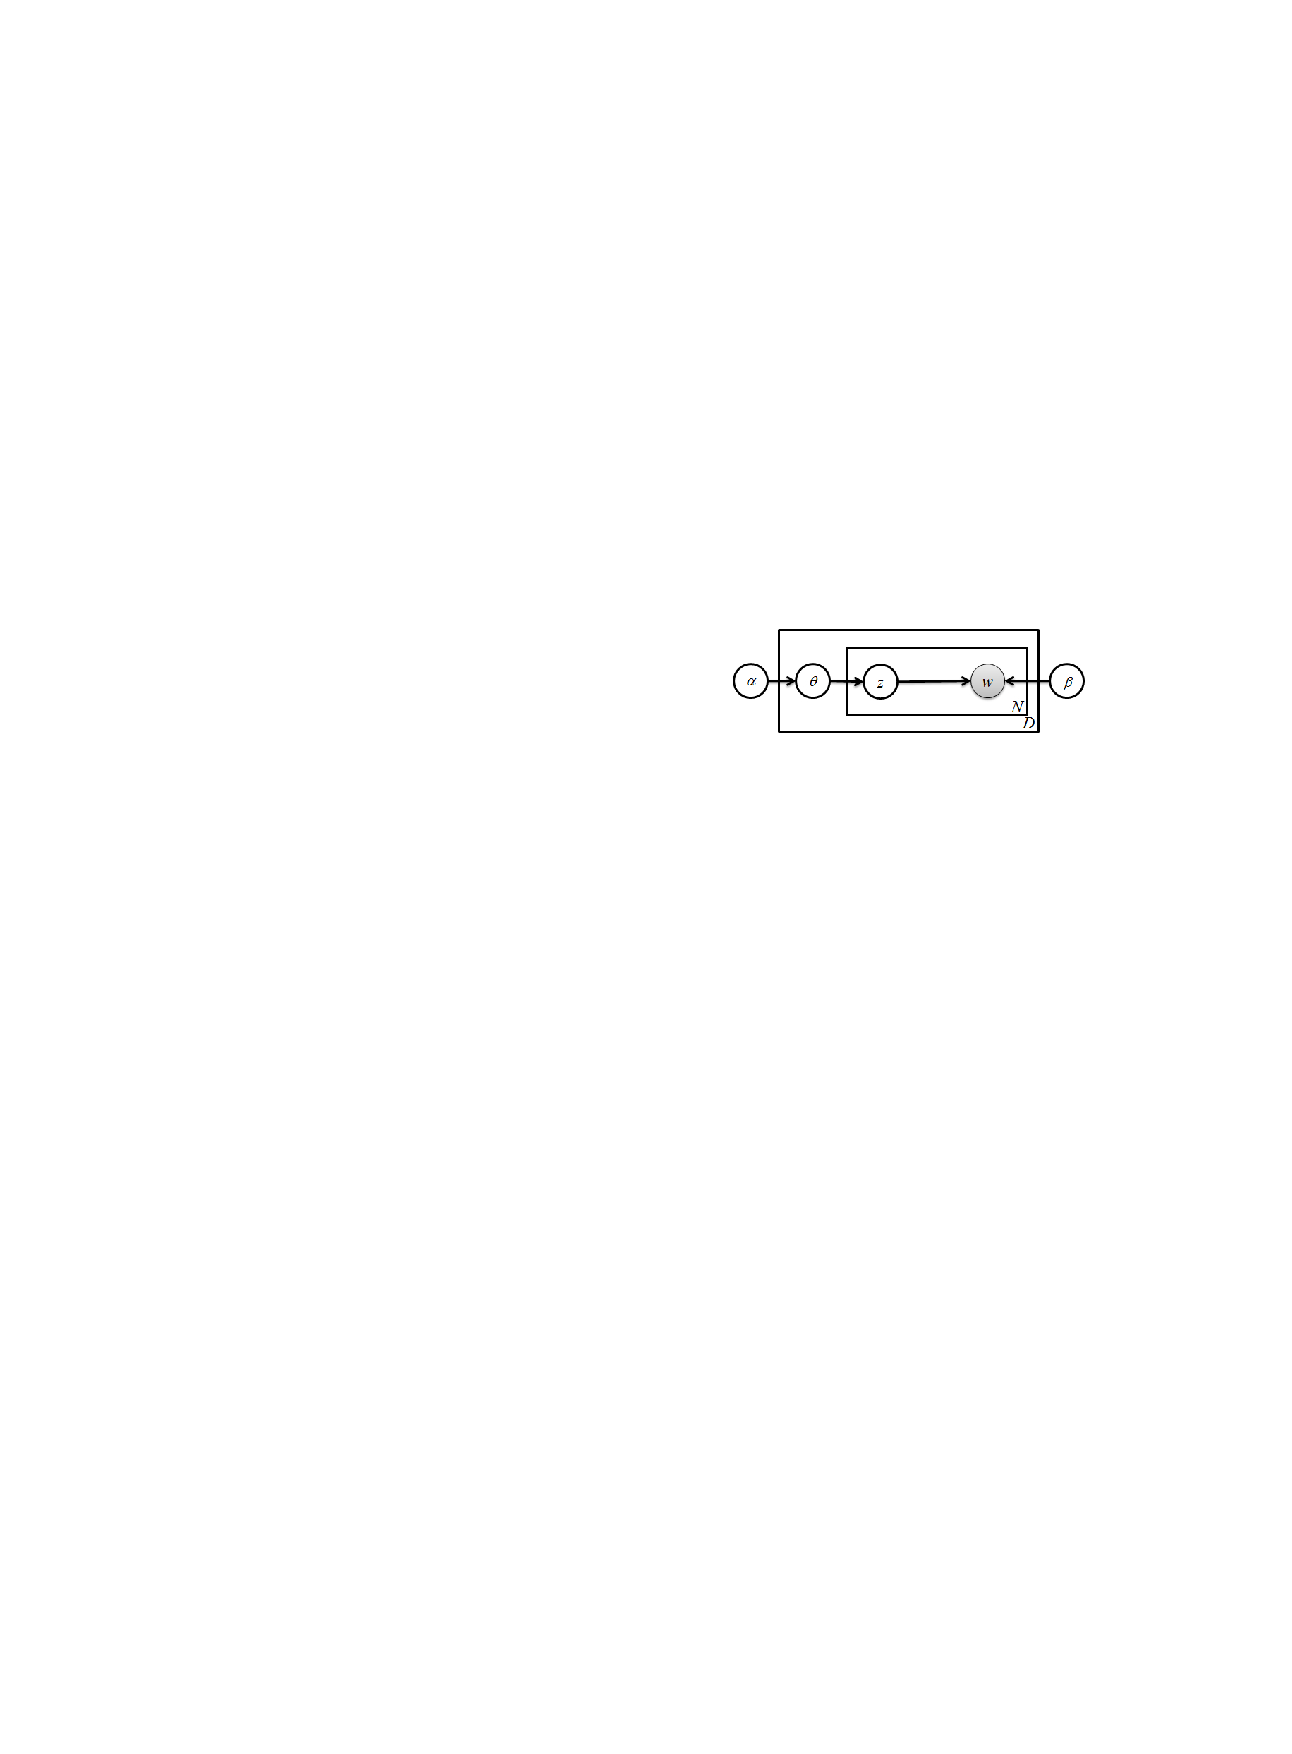
\includegraphics[width=0.5\columnwidth]{figures/methods/LDA_1}
\caption{LDA graphical model. Source of figure: \cite{moghaddam2012design}.}
\label{fig:methods:LDA_1}
\end{figure}

\subsubsection{S-LDA: seperate aspect and rating}

In S-LDA \cite{lakkaraju2011exploiting,moghaddam2012design}, the latent variable for topics $\vz$ is replaced by two seperate variable for aspects and rating respectively. For each aspect-rating pair, $\theta$ contains the probability of generating the corresponding combination. For each review, $\theta$ is sampled once, just like LDA; then $a_n$ and $r_n$ are sampled independently for each word and $w_n$ is sampled conditioned on both latent variable. The formal definition of the generation process is the following, as shown in Figure~\ref{fig:methods:S-LDA}:

$$p(\va, \vr, \vw, \theta | \alpha, \beta) = p(\theta, \alpha) \prod_{n=1}^N \left[ 
p(a_n| \theta) p(r_n | \theta) p(w_n | a_n, r_n, \beta)\right]$$

\begin{figure}
\centering
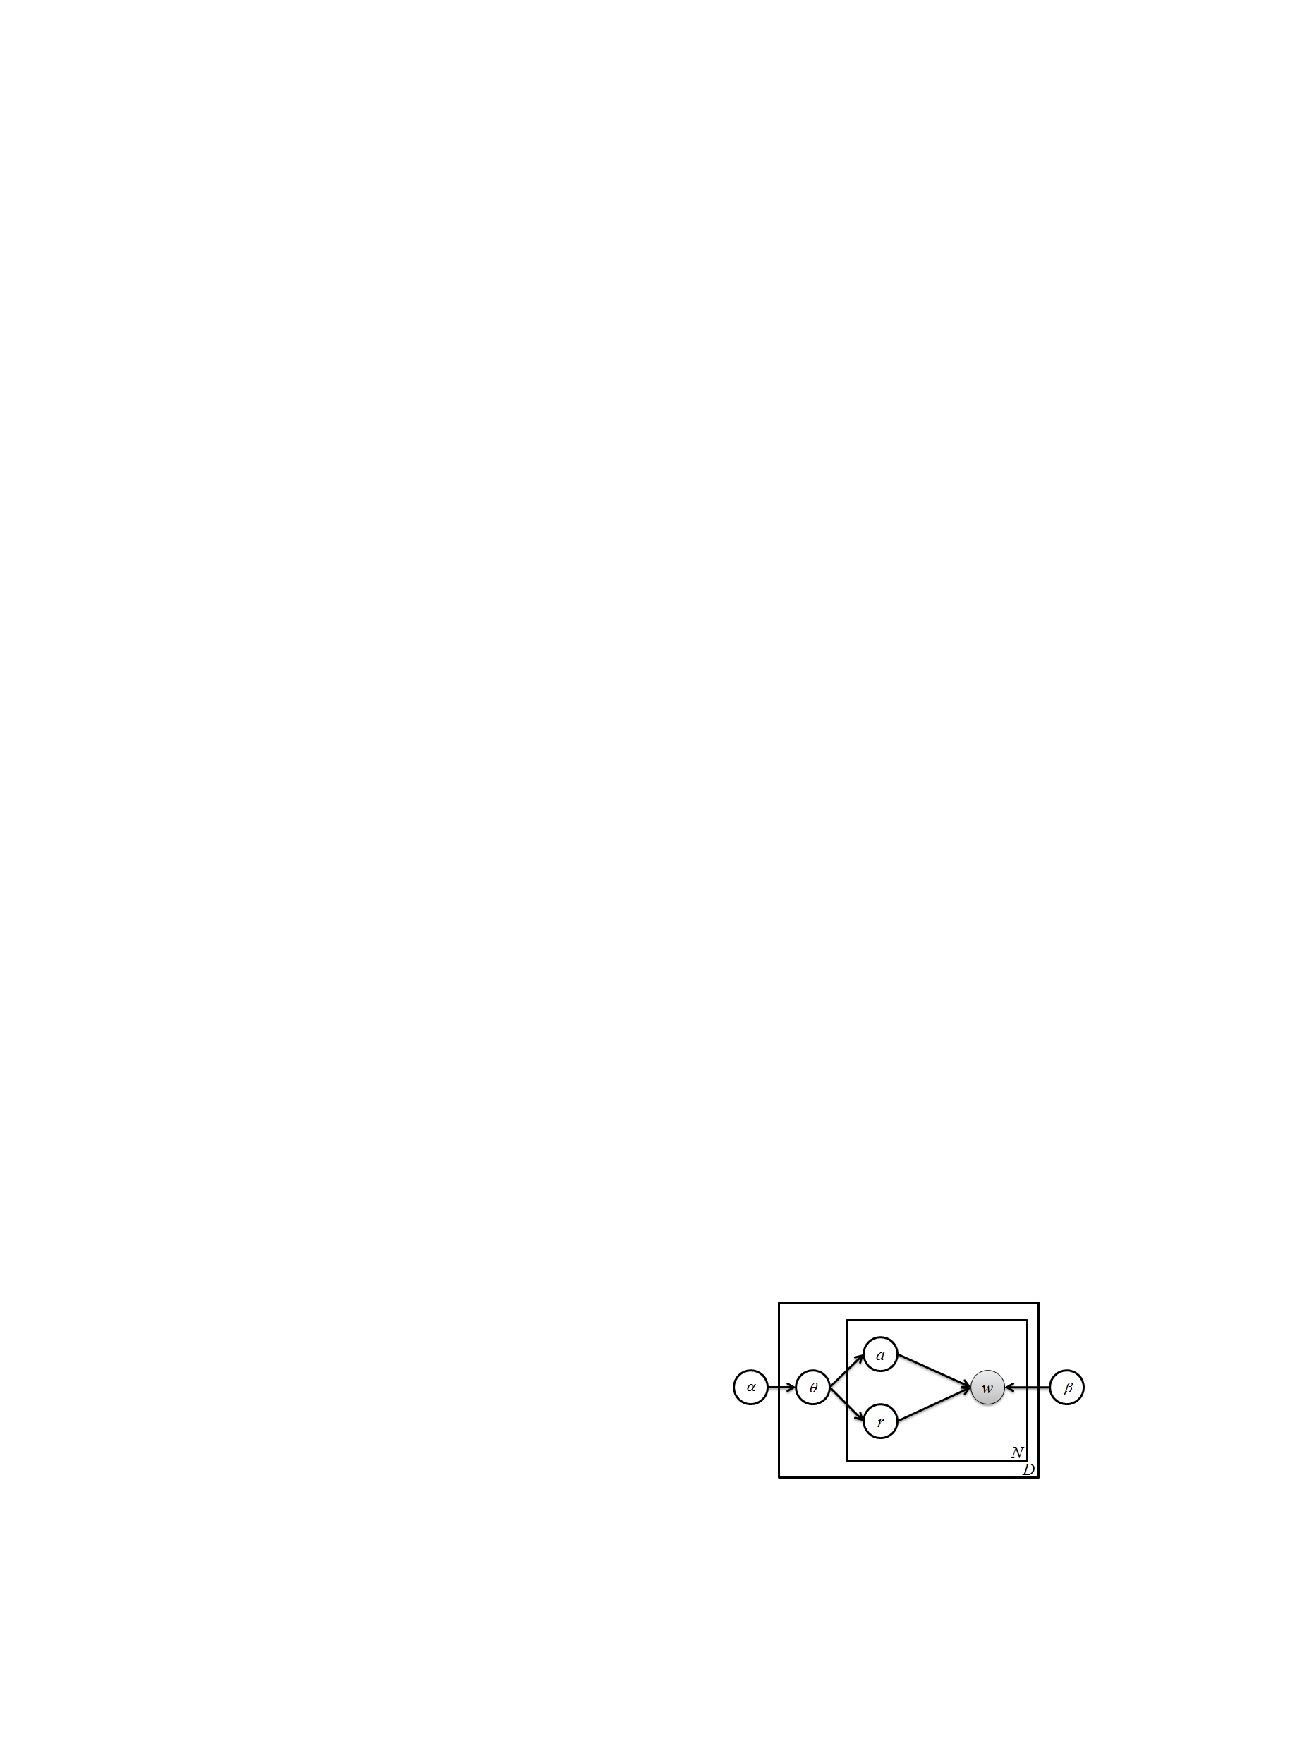
\includegraphics[width=0.5\columnwidth]{figures/methods/S-LDA}
\caption{S-LDA. \cite{moghaddam2012design}}
\label{fig:methods:S-LDA}
\end{figure}

\subsubsection{D-LDA: dependency between aspect and rating}

Several variations of LDA leveraged the dependency between aspects and ratings \cite{he2011automatically,jo2011aspect,li2010sentiment,lin2009joint,moghaddam2011ILDA,moghaddam2012design}.
On the basis of S-LDA, D-LDA further models the dependency of the rating on the aspect. The generation process is the following, as shown in Figure~\ref{fig:methods:D-LDA}:

$$p(\va, \vr, \vw, \theta | \alpha, \beta) = p(\theta, \alpha) \prod_{n=1}^N \left[ 
p(a_n| \theta) p(r_n | a_n, \theta) p(w_n | a_n, r_n, \beta)\right]$$

\begin{figure}
\centering
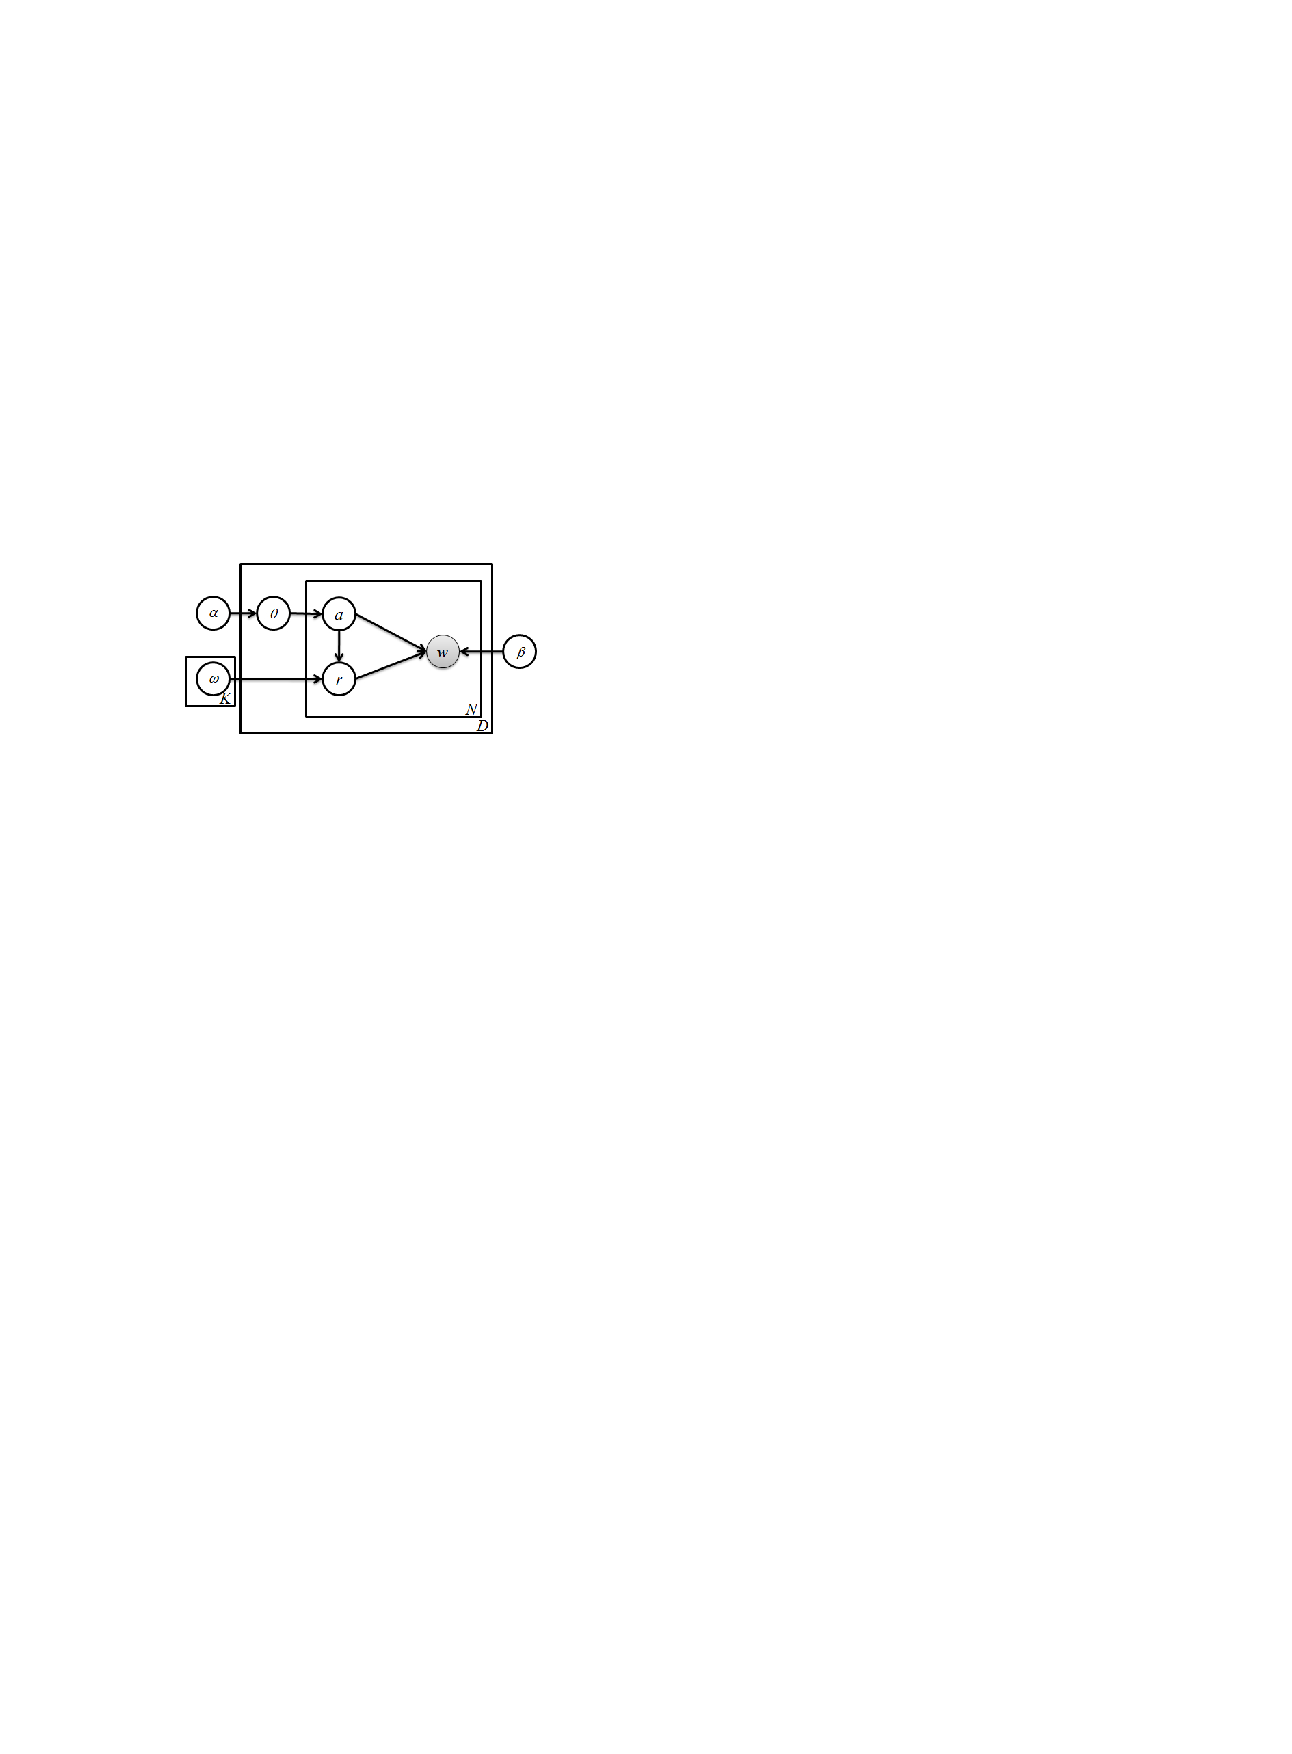
\includegraphics[width=0.5\columnwidth]{figures/methods/D-LDA}
\caption{D-LDA. \cite{moghaddam2012design}}
\label{fig:methods:D-LDA}
\end{figure}

\subsubsection{PLDA: model only opinion phrases}

While LDA assumes that a document is a bag of words, P-LDA \cite{zhan2011semantic,moghaddam2012design} assumes that a document is a bag of opinion phrases. A document is preprocessed to contain only opinion phrases, each being a head-modifier pair $<h_n, m_n>$. Thus, instead of one, the observed variable in P-LDA is two - a head and a modifier, resulting in the generation process as shown in Figure~\ref{fig:methods:P-LDA}:

$$p(\vz, \vh, \vm, \theta | \alpha, \beta, \pi) = p(\theta, \alpha) \prod_{n=1}^N \left[ 
p(z_n| \theta) p(h_n, m_n | z_n, \beta, \pi)\right]$$

\begin{figure}
\centering
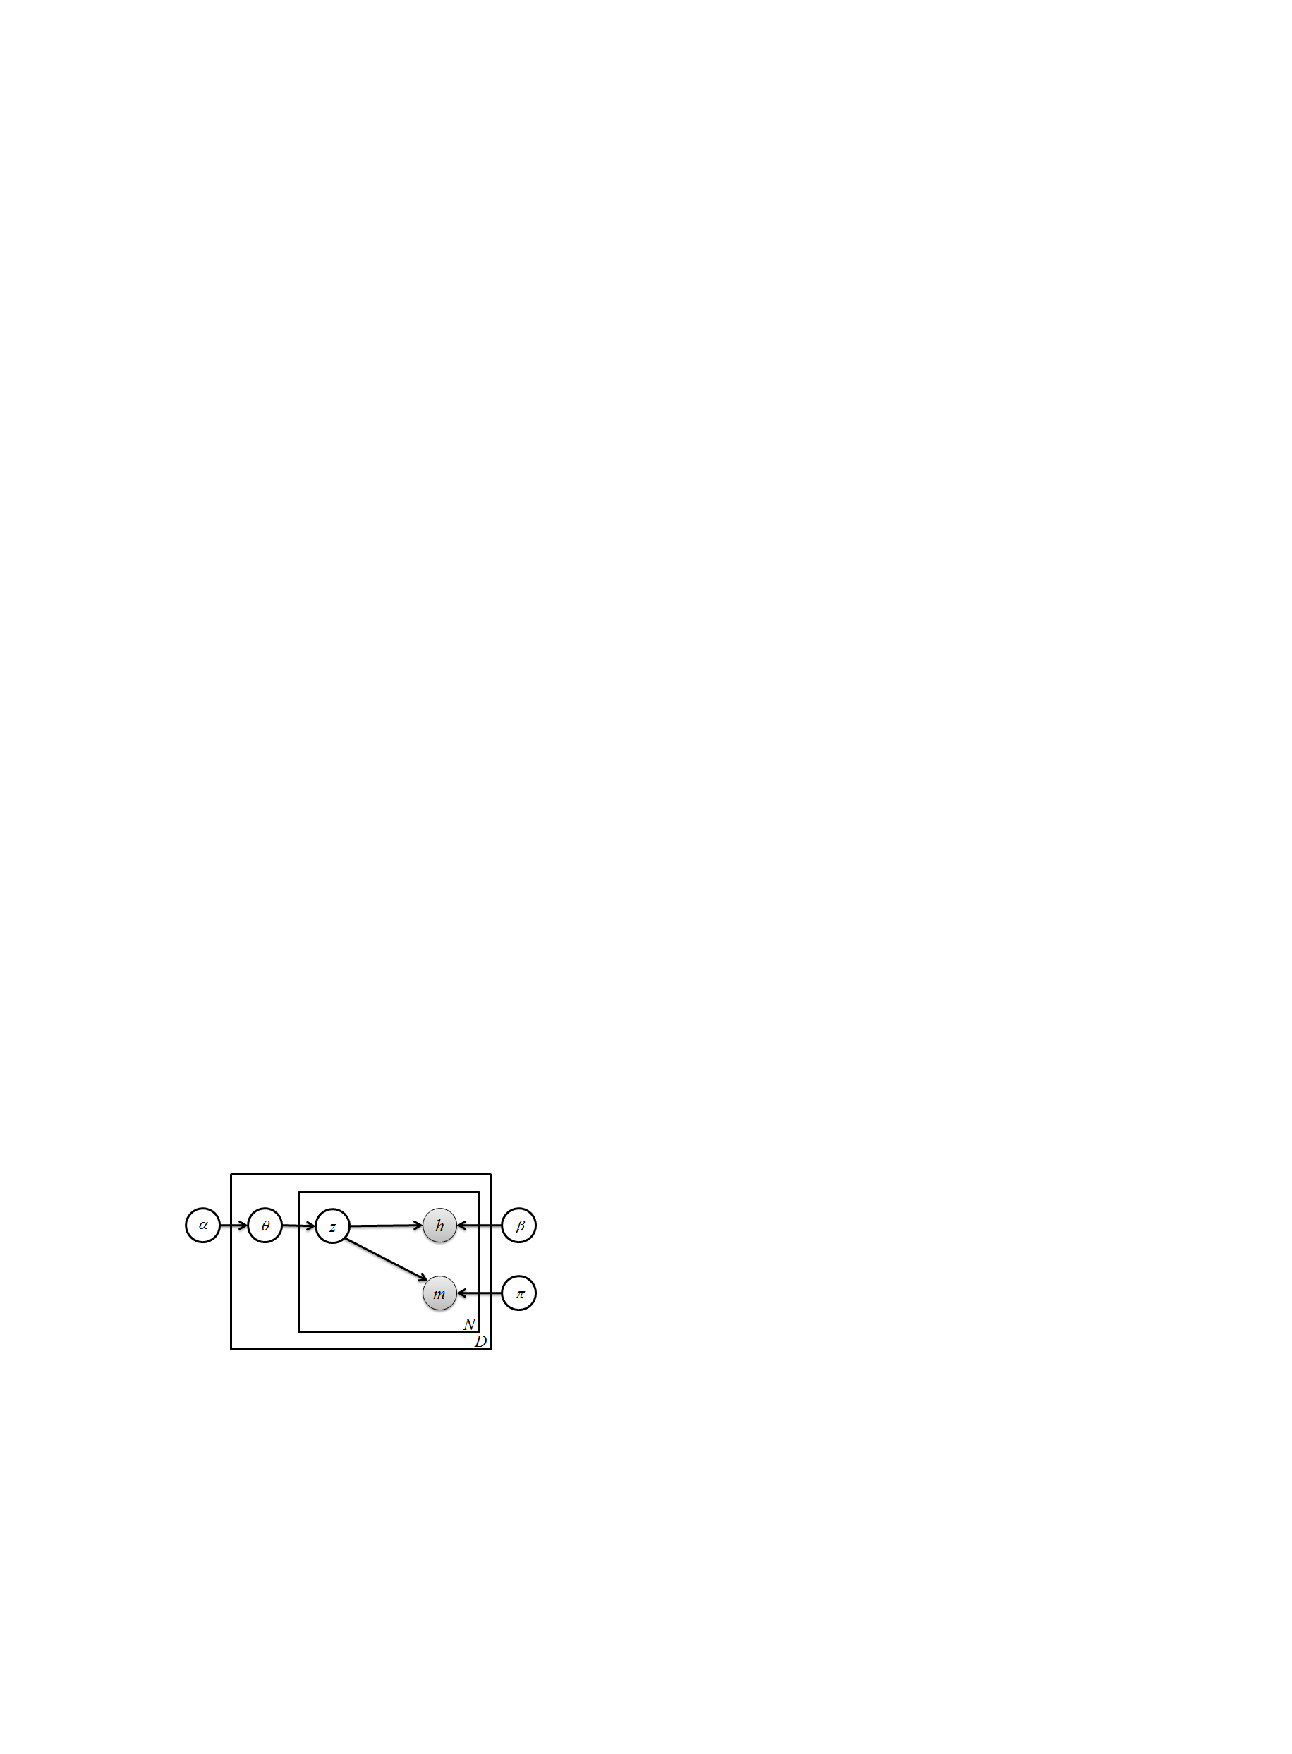
\includegraphics[width=0.5\columnwidth]{figures/methods/P-LDA}
\caption{P-LDA. \cite{moghaddam2012design}}
\label{fig:methods:P-LDA}
\end{figure}

\subsubsection{S-PLDA}

Combining S-LDA and PLDA, we have S-PLDA \cite{moghaddam2012design} as shown in Figure~\ref{fig:methods:S-PLDA}:

$$p(\va, \vr, \vh, \vm, \theta | \alpha, \beta, \pi) = p(\theta, \alpha) \prod_{n=1}^N \left[ 
p(a_n| \theta) p(r_n | \theta) p(h_n | a_n, \beta) p(m_n | r_n, \pi)\right]$$

\begin{figure}
\centering
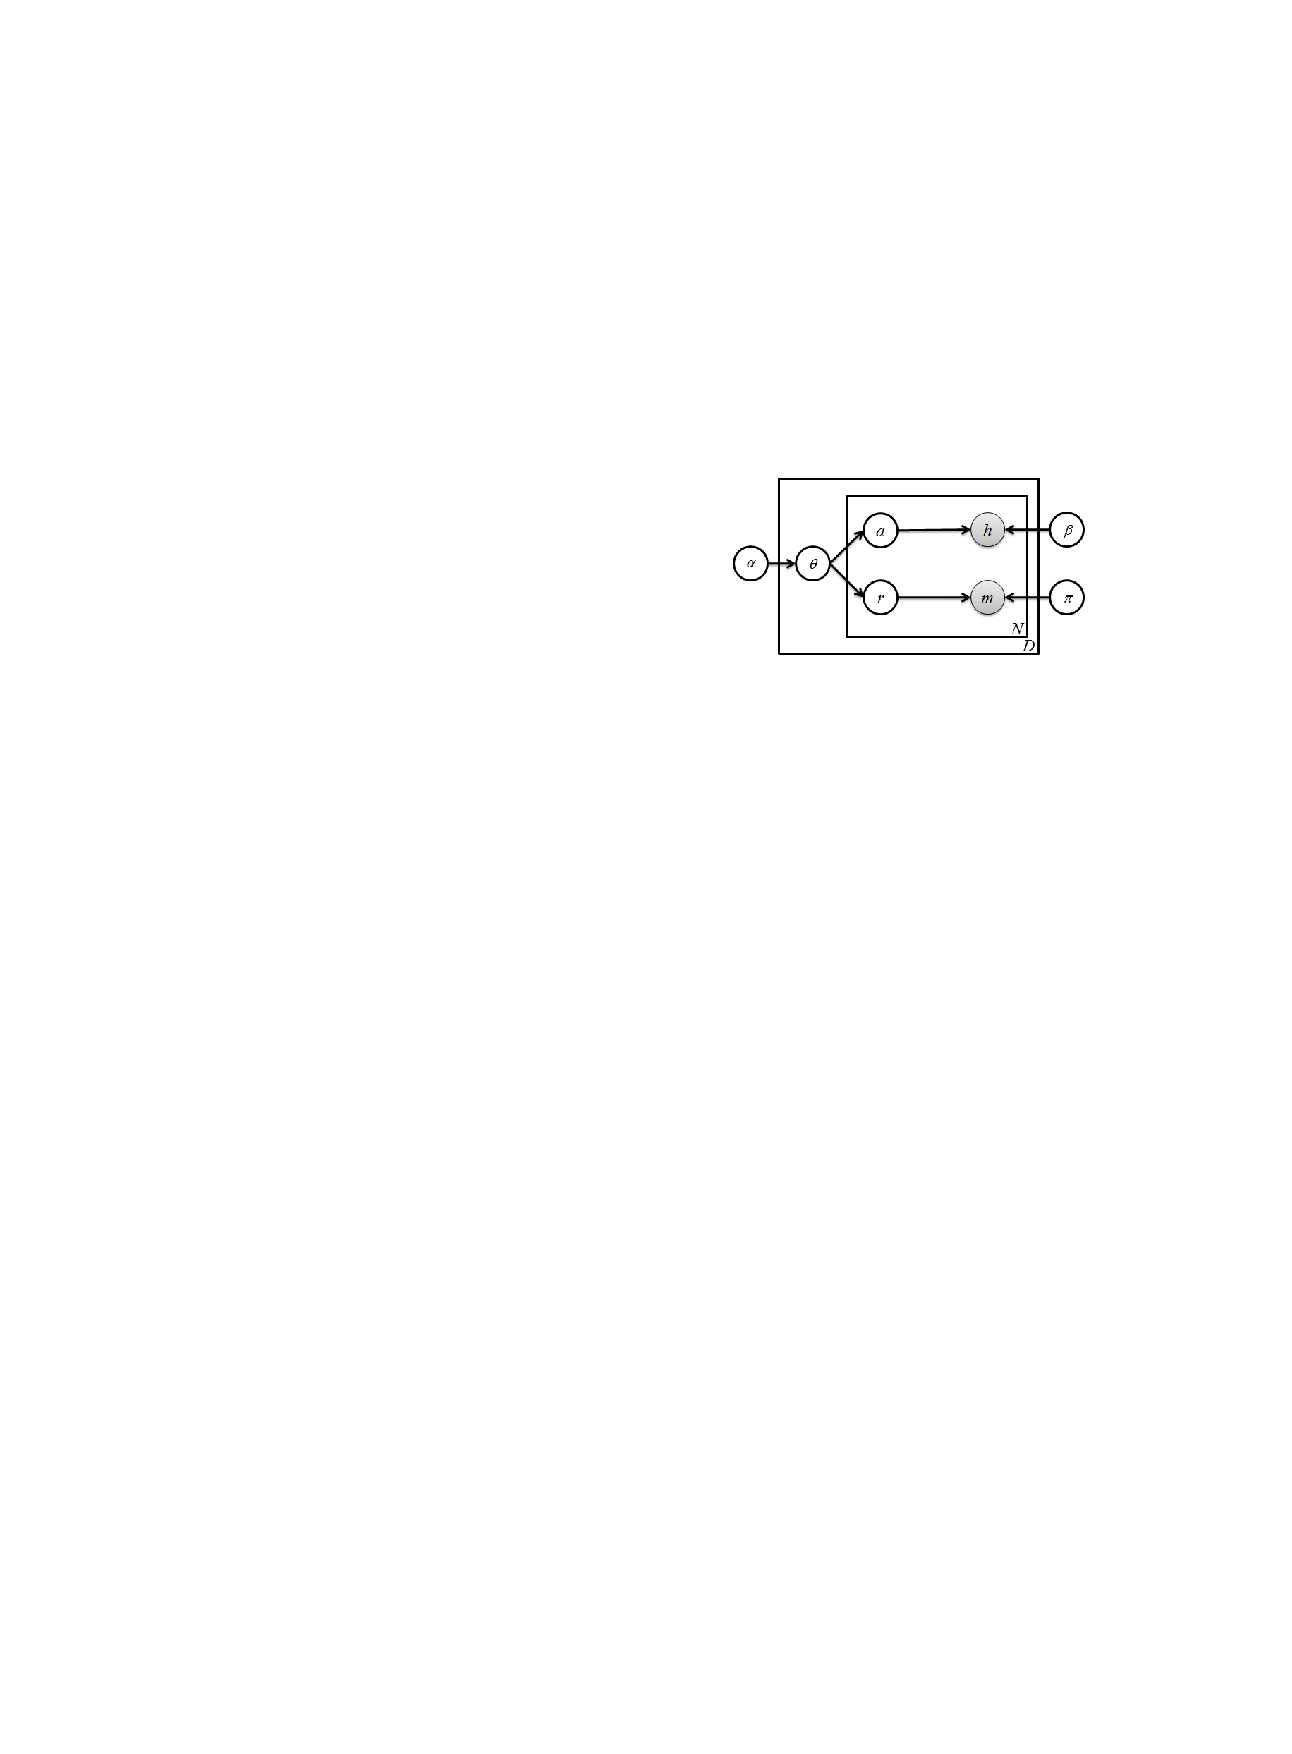
\includegraphics[width=0.5\columnwidth]{figures/methods/S-PLDA}
\caption{S-PLDA. \cite{moghaddam2012design}}
\label{fig:methods:S-PLDA}
\end{figure}

\subsubsection{D-PLDA}

By adding the aspect-rating dependency to S-PLDA, we have D-PLDA \cite{moghaddam2011ILDA,moghaddam2012design}, as shown in Figure~\ref{fig:methods:D-PLDA}:

$$p(\va, \vr, \vh, \vm \theta | \alpha, \beta, \pi) = p(\theta, \alpha) \prod_{n=1}^N \left[ 
p(a_n| \theta) p(r_n | a_n, \theta) p(h_n | a_n, \beta) p(m_n | a_n, r_n, \pi)\right]$$

\begin{figure}
\centering
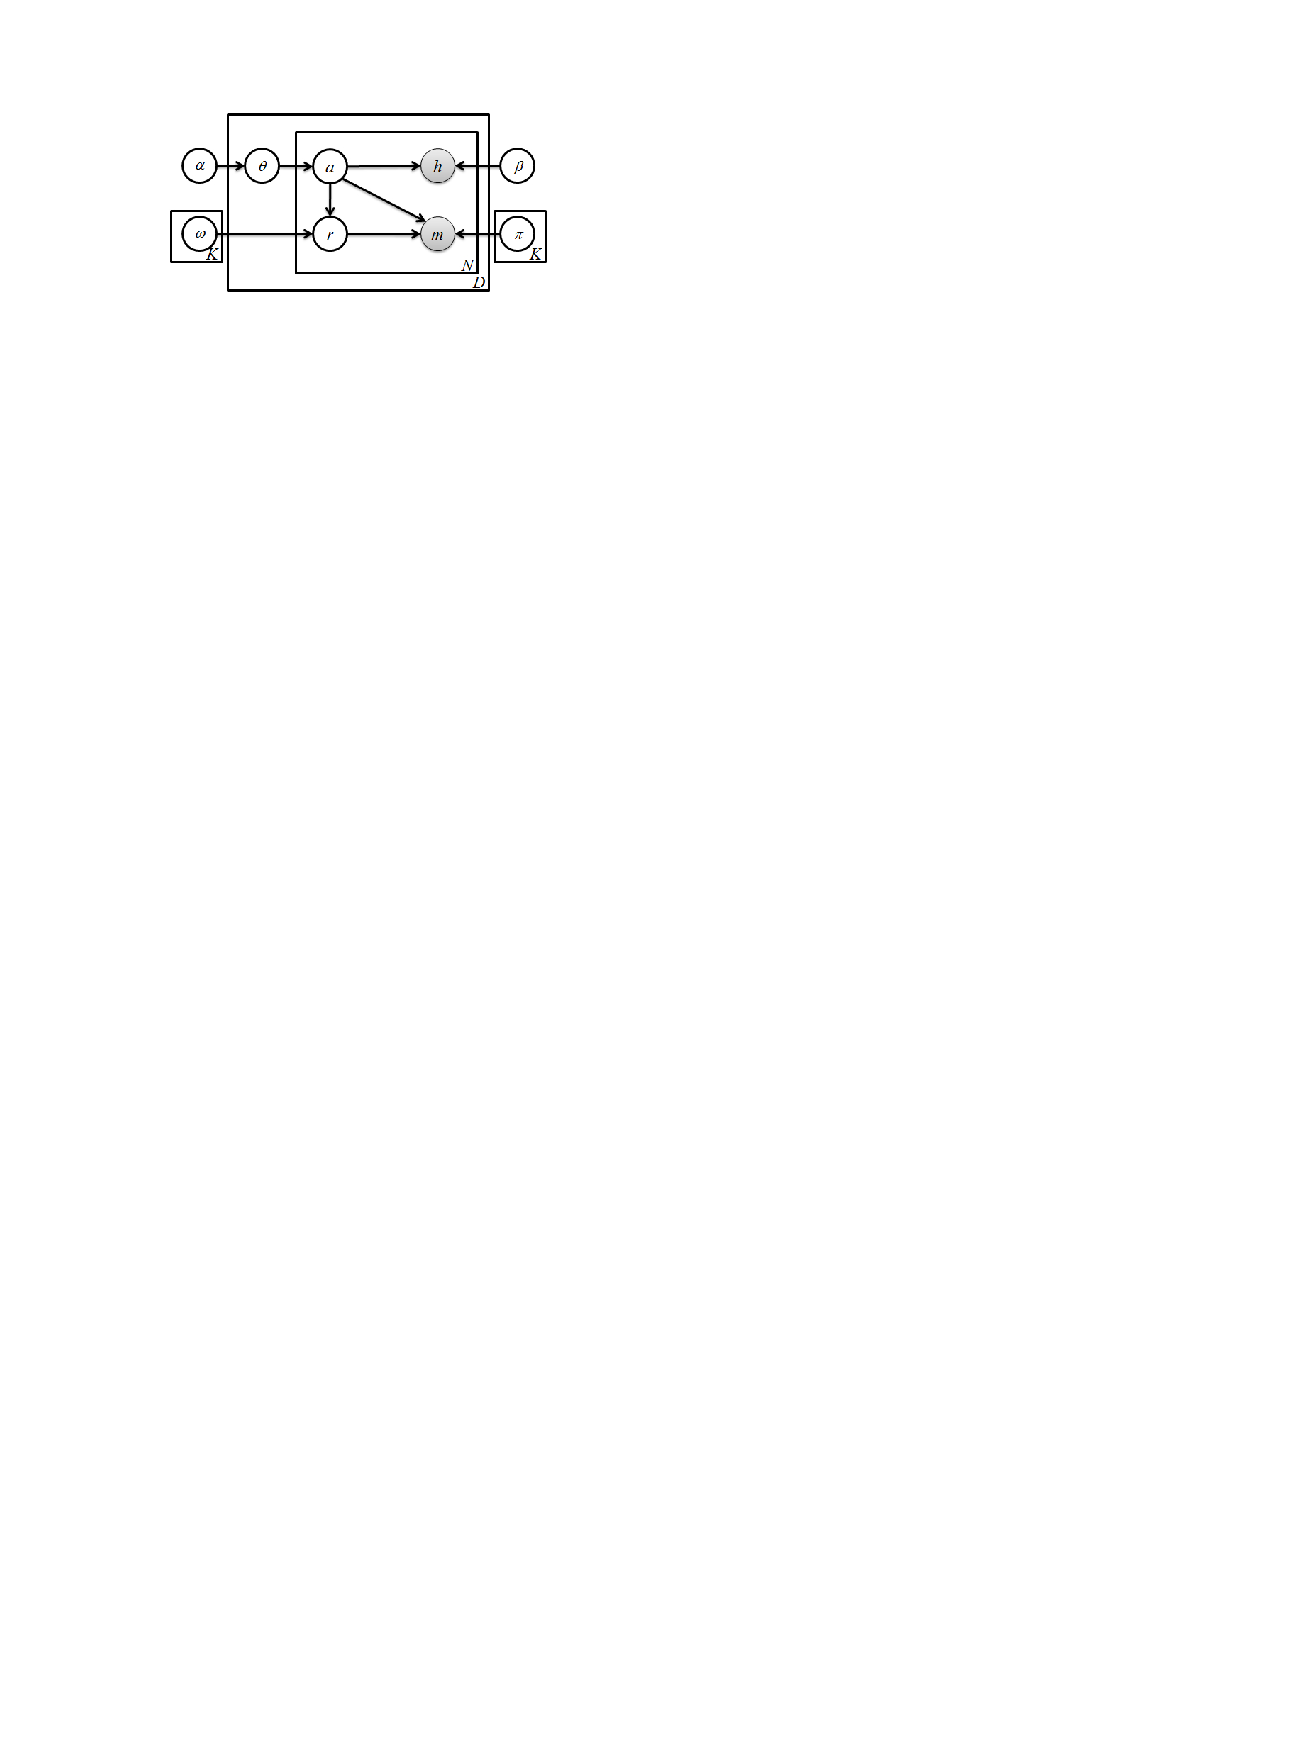
\includegraphics[width=0.5\columnwidth]{figures/methods/D-PLDA}
\caption{D-PLDA. \cite{moghaddam2012design}}
\label{fig:methods:D-PLDA}
\end{figure}

\subsubsection{MG-LDA}

Since aspect extration is a multi-document summarization, the dataset we use is a set of reviews about different products. For example when we perform aspect extraction for hotels, we might use user reviews for different hotel in various cities. Thus in the reviews there are topics that are specific to some particular hotel or a subset of hotels, for example \emph{hotels in Paris}, \emph{youth hostels}. They are valid topics, however not appropriate for ratable aspects. These topics are correlated with the specific product, hence is shared across the scope of the whole review; the topics that can be used as aspects, as analyzed in the previous chapter, are often talked about in segments of the review. The features specific to some product might be prominent at the scope of one review, but if we break down the reivews into sentences, the occurrance of such features specific will be ``diluted" and the aspect topics are more prominent. Motivated by this observation, the authors of MG-LDA \cite{titov2008modeling} introduced two kinds of topics: \emph{local topics} are the ones observed locally in several consecutive sentences, and are appropriate as aspects; \emph{global topics} are the ones closely related to the product and shared across a single review. The generation of words is thus different from that of LDA: now we use a combination of two topic distribution, one global topic that determines the features specific to the product we review, and a local topic that determines which aspect of the product we will talk about. The structure of MG-LDA is shown in Figure~\ref{fig:methods:MG-LDA}. For each document, the global topic distribution is sampled once, since only target product is consistent throughout the review; the local topic distribution is sampled for each sliding window, thus is sampled multiple times across the review, representing the aspect shifting from window to window; each word in a single window is generated by sampling from both topic distributions and combining them.
\begin{figure}
\centering
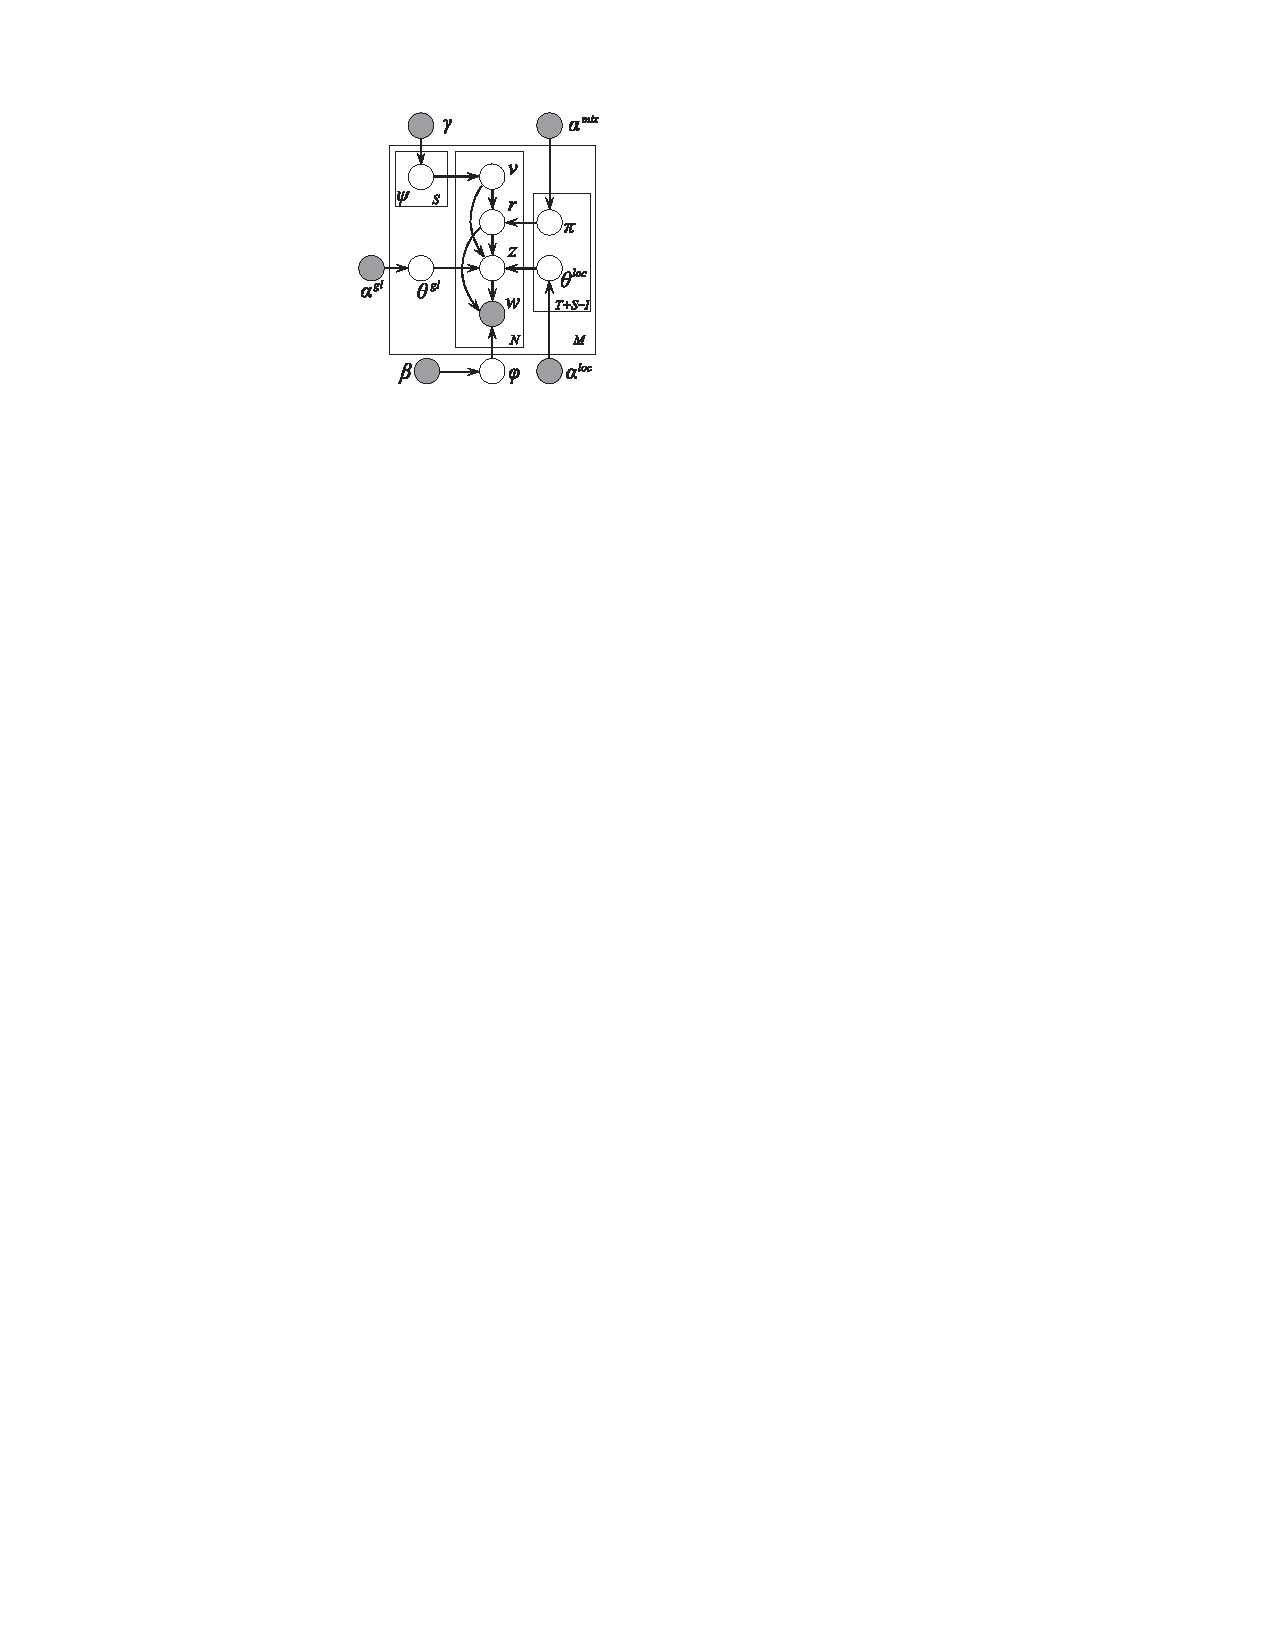
\includegraphics[width=0.5\columnwidth]{figures/methods/MG-LDA}
\caption{MG-LDA. Source of figure: \cite{titov2008modeling}.}
\label{fig:methods:MG-LDA}
\end{figure}

MG-LDA was designed specifically for aspect extraction, without distinguishing aspects and sentiments. MG-LDA has been shown to perform better than other LDA variations mentioned above, so we will make a direct comparison with our model  in our experiment chapter.

\section{Deep Learning for Natural Language Processing}


\begin{displayquote}
 ``Deep Learning waves have lapped at the shores of computational linguistics for several years now, but 2015 seems like the year when the full force of the tsunami hit the major Natural Language Processing (NLP) conferences." - Dr. Christopher D. Manning, Dec 2015 
\end{displayquote}

Deep learning has drawn a lot of attentiono in recent years, and we have already seen many applications of it in natural language processing. In this section we will first give a brief introduction to the history of deep learning; then we will introduce several widely used deep learning methods for natural language processing. 

\subsection{A Brief History of Deep Learning}

The core model of deep learning is neural network. The earliest neural-network-like algorithms that had multiple layers of no-linear features can be traced back to \cite{ivakhnenko1965cybernetic}, where the authors used a thin but deep models with polynomial activation functions which they analyzed with statistical methods. In each layer, they select the best features through statistical methods and forward them to the next layer. They did not use backpropagation to train their network end-to-end but used layer-by-layer least squares fitting where previous layers were independently fitted from later layers.

The earlist convolutional network appeared in \cite{fukushima1979organization}. Their networks had multiple convolutional and pooling layers similar to modern networks, but the network was trained by using a reinforcement scheme where a tail of strong activationo oin multiple layers was increased over time.

Backpropagation of erros that are used to train deep models was lacking at this point. It was derived already in the early 1960s but in an inefficient and incomplete form. The modern form was derived first by Linnainmaa in his 1970 masters thesis, however he did not mention its application to neural networks. Even at this point, backpropagation was relatively unknown and very few documented applications of backpropagation in the early 1980s. \cite{rumelhart1988learning} showed that backpropagation used for neural networks could yield interesting distributed representations. At this time, this was an important result in cognitive psychology where the questiono was whether human cognition can be thought of as relying on distributed representations (connectionism) or symbolic logic (computationalism).

The first practical application of backpropagation cam about through \cite{lecun1989backpropagation} where the authors used convolutional networksin combination with backpropagation to classify handwritten digits (MNIST) and this system was later used to read large numbers of handwritten checks in the United States. Despite these successes, funding for research into neural networks was scarce. The term artificial intelligence dropped to near pseudoscience status during the ``AI winter". Some important advances were made in this time, for example, long short-term memory (LSTM) for recurrent neural network \cite{hochreiter1997long}, but these advances went mostly unnoticed util later as they were overshadowed by support vector machine (SVM) \cite{cortes1995support}.

The next big shift occured just by waiting for the computers to get fater, and then later by the introduction of GPU. In this period, neural networks slowly began to rival SVMs. The main difficulty at this point was to train big, deep networks, which suffered from vanishing gradient problem, where features in early layers could not be learned because no learning signal reached these layers.

The first solution to this problem was layer-by-layer pre-training, where the model is built in a layer-by-layer fashion by using unsupervised learning method. The first pre-training approaches was proposed for recurrent neural networks by \cite{schmidhuber1992learning}, and then for feed-forward networks by \cite{hinton2006reducing}, which started the fever of neural networks.

\subsection{Word2Vec}

As natural language processing often treats words as the basic unit of study and neural networks takes vectors as input, it is natural to represent words by vectors. The most basic model is one-hot vector, where each vector has the size of the vocabulary, and one non-zero entry denoting the word. This simple design has several drawbacks: first it's dimensionality is too large if we have a large dictionary; secondly and more importantly, the vector representation does not capture any semantic information of the words. To improve the vector representation of words, we replace the original high-dimensional discrete vector with a lower-dimensional real-valued vector; instead of the pre-defined fixed values, we train the vector representations so that the cosine similarity of two word vectors captures the semantic similarity of the two corresponding words. This Word2Vec \cite{mikolov2013distributed} model adopted a heuristic: if two words often appear close to each other, then they are similar, and this is called word embedding - embed a word's meaning in the the words surrounding it. Also, the semantics of each word is stored in all the entries of the word vector, so the word vector we learned is called a \emph{distributed representation}.

Word2Vec contains two seperate models: skip-gram and CBOW. The two models can used independently two train two vectors for each word, and concatenate the two vectors to obtain the final word embedding. However in practice, people often use only the skip-gram model with special training techniques like negative samping and noise contrastive estimation. In our paper, we introduce skip-gram with negative sampling.

For a high level interpretation, we consider a single word $w$ in a sentence: skip-gram asks us to predict each other word, or context word $c$, in the sentence with $w$; this way we embed the meaning of the context in the representation of $w$. For a more formal definition, we consider all the word-context pairs $(w,c)$ in a corpus $D$, and we consider the conditional probabilities $p(c|w)$. We use $C(w)$ to denote the set of contexts of word $w$, and $\theta$ as the parameters of $p(c|w; \theta)$. Our goal is to find the parameters that maximize the corpus probability.

$$\theta = \argmax_{\theta} \prod_{w\in W} \left[\prod_{c\in C(w)} p(c|w; \theta) \right]\text{;  or alternatively}$$
$$\theta = \argmax_{\theta} \prod_{(w,c)\in D} p(c|w; \theta)$$

When predicting each context word $c$ with word $w$, the model uses a softmax:

$$p(c|w;\theta) = \frac{e^{v_c\cdot v_w}}{\sum_{c'\in C}e^{v_{c'}\cdot v_w}}$$

where $v_c, v_w, v_{c'} \in \mathbb{R}^d$ are vector representations of $c, w, c'$ respectively; $C$ is the set of all available contexts. Maximizing the above conditional probability is equivalent to maximizing the objective:

$$\argmax_{\theta}\sum_{(w,c)\in D} \log p(c|w)
= \sum_{(w,c)\in D} (\log e^{v_c\cdot v_w} - \log\sum_{c'\in C}e^{v_{c'}\cdot v_w})$$

While the above objective can be computed, but it's computationally expensive to do so, because the summation will iterate over all the contexts $c'$. One way of making the computation more tractable is to replace the summation with a sampling of random noises, this is called negative sampling. Note that other methods like noise contrastive estimation \cite{mnih2013learning} and importance sampling \cite{bengio2003quick,bengio2008adaptive} all share the same basic idea, and we will not elaborate on thess two other models in this paper.

With negative sampling, the model is actually optimizing a different objective. Consider a word-context pair $(w,c)$, we denote by $p(D=1|w,c)$ the probability that $(w,c)$ came from the corpus, correspondingly, $p(D=0|w,c)=1-p(D=1|w,c)$ denotes the probability did not come from the corpus. Still with parameters $\theta$, our goal is now to maximize the probabilities that all the observed pairs indeed came from the corpus:

\begin{align*}
    &\argmax_{\theta}\prod_{(w,c)\in D} p(D=1|w,c;\theta) \\
    &=\argmax_{\theta} log \prod_{(w,c)\in D} p(D=1|w,c;\theta) \\
    &=\argmax_{\theta} \sum_{(w,c)\in D} \log p(D=1|w,c;\theta)
\end{align*}

The conditional probability $p(D|w,c|\theta)$ is defined using softmax:

$$p(D=1|w,c;\theta)=\frac{1}{1+e^{-v_c\cdot v_w}}$$

leading to the objective:

$$\argmax_{\theta}\sum_{(w,c)\in D}\log \frac{1}{1+e^{-v_c\cdot v_w}}$$

This objective has a trivial solution if we set $\theta$ so that $v_c=v_w$ and $p(D=1|w,c;\theta)=1$ all the time. But we of course don't want all the words share a same representation and we will disallow some $(w,c)$ pairs. One way to do so is to make $p(D=1|w,c;\theta)$ low for some pairs, i.e. pairs not observed in the data. This is achieved by generating the set $D'$ of random $(w,c)$ pairs and assuming they are out of the corpus - hence ``negative samples". Let $\sigma(x)=\frac{1}{1+e^{-x}}$, the new objective is:

\begin{align*}
    &\argmax_{\theta}\prod_{(w,c)\in D} p(D=1|w,c;\theta) \prod_{(w,c)\in D'}p(D=0|w,c;\theta) \\
    =&\argmax_{\theta}\prod_{(w,c)\in D} p(D=1|w,c;\theta) \prod_{(w,c)\in D'}(1-p(D=1|w,c;\theta)) \\
    =&\argmax_{\theta}\sum_{(w,c)\in D} \log p(D=1|w,c;\theta) + \sum_{(w,c)\in D'} \log(1-p(D=1|w,c;\theta)) \\
    =&\argmax_{\theta}\sum_{(w,c)\in D} \log\sigma(v_c\cdot v_w) + \sum_{(w,c)\in D'} \log\sigma(-v_c\cdot v_w)
\end{align*}

This model can then be trained end-to-end much more efficiently and the final parameters $\theta$ contains all the word vectors. This objective has been shown to be equivalent to factorizting a shifted PMI matrix \cite{levy2014neural}, which means that the semantic similarity captured by Word2Vec is actually the point-wise mutual information between the pair of words. Their are other models of vector representation for words, including \cite{pennington2014glove,shazeer2016swivel}, but Word2Vec is by far the most widely used word vector in applications.


\subsection{Neural Network Language Model}

The goal of statistical language model is to learn the joint probability function of sequences of words in a language. This is difficult due to the curse of dimensionality: there are too many possible sequences. Traditional approaches based on n-grams obtain generalization ability by concatenating very short overlapping sequences, focusing on only a local window each time. In neural network language models, the index-based word representation used in traditional n-gram models is replaced with distributed representations like Word2Vec. This allows the model to be informed about an exponential number of semantically neighboring words each time, due to the semantic embedding in each word vector. With word vectors, the model simultaneously learns the representation of each word and the probability function of the sequence. The generalization ability is improved because each word now shares its information with many other similar words, replacing a word in a already seen sequence with a semantically similar word will now result in a similar probability function.

A statistical language model can be defined by the conditional probability of the next word given previous words: $p(w_1^T) = \prod_{t=1}^T p(w_t | w_1^{t-1})$. The earliest neural network language model was proposed in \cite{bengio2000a} and follows the n-gram approach, which means that it approximate the conditional probability:

$$p(w_t | w_1^{t-1}) \approx p(w_t | w_{t-n+1}^{t-1})$$

The modeling of function $f(w_t,..., w_{t-n+1}) = p(w_t | w_1^{t-1})$ is done by two steps:

\begin{itemize}
    \item[1.] By using a matrix $C$ of shape $|V|\times m$, where $V$ is the vocabulary and $m$ is the dimension of word vector, we map the input sequence $(w_{t-n+1}, ..., w_{t-1})$ to a sequence of word vectors $(C(w_{t-n+1}), ..., C(w_{t-1}))$;
    \item[2.] A function $g$ maps the input sequence of word vectors to a conditional probability distribution over all the words in $V$ for the next word $w_t$. The output is a probability vector whose $i$th element estimates $p(w_t=i|w_1^{t-1})$.
\end{itemize}
$$f(i, w_{t-1}, ..., w_{t-n+1}) = g(i, C(w_{t-1}), ..., C(w_{t-n+1}))$$

Note that among the two mappings $g$ and $C$, the later is shared across all the words in the context, holding all the $|V|$ word vectors in rows. Function $g$ is designed to be a feed-forward neural network with parameters $\omega$, so the whole parameter set is $\theta={C, \omega}$. The objective is to minimize the log-likelihood of the entire corpus ($T$ word sequences):

$$L=\frac{1}{T} \sum_t \log f(w_t, w_{t-1}, ..., w_{t-n+1}; \theta) + R(\theta)$$

where $R(\theta)$ is a regularization term designed for avoiding over-fitting of the neural network. 

The input layer of the network receives the sequence of words, map them into a sequence of word vectors and pass it to a normal tangent hidden layer and obtain the outputs $y_i$ for word $i$. The output layer, similar to what is used in skip-gram in Word2Vec, is a softmax output layer:

$$p(w_t | w_{t-1}, ..., w_{t-n+1}) = \frac{e^{y_{w_t}}}{\sum_i e^{y_i}}$$

where $y$ is given by the hidden layer computation:

$$y=b+Wx+U\tanh(d+Hx)$$

where the hyperbolic tangent is applied element-wise; $x$ is the concatenation of the input word vectors:

$$x=(C(w_{t-1}), C(w_{t-2}), ..., C(w_{t-n+1}))$$

The whole model is then trained end-to-end, simultaneously learning the representation of words and the probability function for sequences.

The model has several restrictions to this language model that is based on a feed-forward neural network. First the computational cost at the softmax layer is very high, similar to what we see from Word2Vec, but this time we cannot directly use negative sampling, because we need to consider the $n-1$ previous words, instead of only one word. Importance sampling can be applied to this scenario with some careful modification \cite{cho2015on}. Another way to solve this problem is to replace the flat softmax with some hierarchical structure, that is, using a hierarchical softmax \cite{mikolov2013efficient}. Also the normalization of the softmax can be replaced by a self-normalizing term learned jointly with the model \cite{devlin2014fast}. Beside the computational efficiency, this model is restricted to using local features - only previous $n-1$ words are used for predicting the next word. To address this problem, we adopt recurrent neural network, which is specifically designed for modeling sequences of different lengths.

\subsection{Recurrent Neural Network}

The idea behind recurrent neural network (RNN) is to make use of sequential information. In traditional layer structured neural network, we assume that all inputs (and outputs) are independent of each other. But for tasks like language modeling this is a huge restriction. RNN is ``recurrent" because it performs the same process for every element in a sequence, with the output being depended on the previous computations. Another way to think about RNN is that it has a ``memory" which captures imformation about what has been calculated so far. In theory RNN can make use of information in arbitrarily long seuqnces, but inpractive they are limited to looking back only a few steps.

The computation of RNN is slightly different from normal neural network which is a stack of layers, instead of going through the fixed structure of layers, RNN carry out its computation in multiple time steps. The time steps of RNN actually correspond to the layers of normal neural network, however the depth of layers is not pre-defined and varys according to the input sequence. RNN has two core functions which it performs at each time step: update of its internal state, and output based on its internal state; the later is optional.

The abstraction of RNN internal state update is simple: $h_t=\RNN(h_{t-1}, x_t)$, where $h_t$ is the new state, $h_{t-1}$ is the previous state, $x_i$ is the input at this time step, all of them are vectors; $\RNN$ encapsules the computation of an RNN layer, which in the most simple form is just linear transformations followed by a non-linearity (biases are dropped for simplicity):

$$RNN(h_{t-1}, x_t) = tanh(Wh_{t-1} + Ux_t)$$

The output part of RNN is also simple. Let us consider the scenario of language modeling. At each time step $t$ we have a hidden state $h_t$ which contains the information of all previous words $(x_1, ..., x_t)$. With this state we can predict the next word $x_{t+1}$ by computing a softmax over all possible words, which gives us the probability of next word $x_{t+1}$ conditioned on the previous words, therefore we can model the probability of the whole sequence with this RNN. After training the RNN for language modeling, it can be further used for generating sequences: at each time, take the word with the highest probability predicted by the softmax; then feed the predicted output to the RNN as an input; proceed until the RNN outputs a special symbol denoting the end of the sequence.

\begin{figure}
\centering
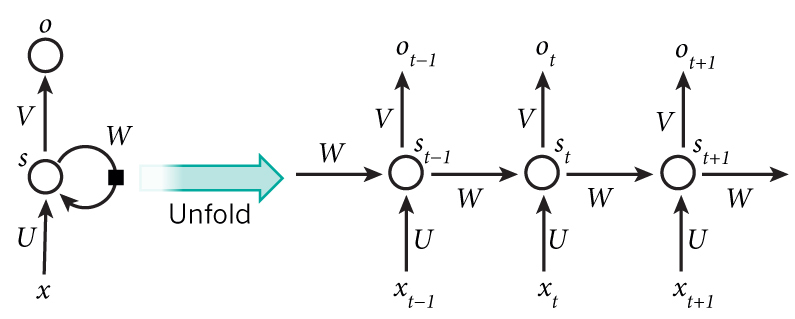
\includegraphics[width=0.7\columnwidth]{figures/methods/RNN}
\caption{The rolled and unrolled forms of RNN. Source: \emph{Nature}.}
\label{fig:methods:RNN}
\end{figure}

The rolled and unrolled forms of RNN is shown in Figure~\ref{fig:methods:RNN}. It is important to remember that almost all RNN structures follow the abstraction above, though the instantiation of the $\RNN$ function might be much more complicated. With this abstraction, we can see the correspondence between RNN and a traditional neural network structure: the hidden states of RNN correspond to the activations of a normal NN's hidden layers, but the parameters are shared across layers. This correspondence leads us to the training algorithm for RNN - backpropagation through time (BPTT). After unrolling the RNN computation into layers similar to normal NN, we do backpropagation just like normal; but after updating the weights at all the layers - which are actually copies of a single layer, we take the average of those copies and use it as the new RNN layer.

Since RNN and normal NN use virtually the same training algorithm, the difficulty of training a deep neural network also occurs to RNN when the input sequence is long and the depth of RNN is correspondingly large. The main problem is the vanishing gradient problem \cite{hochreiter1991untersuchungen,hochreiter2001gradient}. The intuitive explaination of vanishing gradient is: RNN updates involves repeatedly multiplying a matrix to itself, and when the matrix entries are small, almost no gradient is passed to earlier layers. The result is: information learned at later time steps cannot be efficiently passed to earlier time steps, making it hard for RNN to learn long-distance dependencies in the sequence. Detailed analysis of the vanishing gradient problem can be found in \cite{pascanu2013on}. This problem makes RNN less useful for something like language modeling, which often involves long input sequences.

\subsubsection{Long Short-Term Memory}

Long Short-Term Memory \cite{hochreiter1997long} is a variation of RNN that is designed to address the vanishing gradient problem. The abstraction of LSTM is still the same to the original one: $h_i=\RNN(h_{t-1}, x_t)$; however the update function $\RNN$ is more complicated. LSTM introduced four new elements: input gate $i$, forget gate $f$, output gate $o$, and cell $c$; the formal update function is:

\begin{align*}
& i_t = \sigma(W^i x_t + U^i h_{t-1}) \\
& f_t = \sigma(W^f x_t + U^f h_{t-1}) \\
& o_t = \sigma(W^o x_t + U^o h_{t-1}) \\
& c_t = f_t \odot c_{t-1} + i_t \odot \tanh(Wx_t + Uh_{t-1}) \\
& h_t = o_t \odot \tanh(c_t)
\end{align*}

where $\sigma$ is the sigmoid function, $\odot$ denotes the element-wise product.

Despite the seemingly complicated design, there is a clear intuition behind LSTM. LSTM can be derived from normal RNN by two steps:

\begin{itemize}
    \item[1.] In the original RNN, the repeated multiplication introduced the vanishing gradient problem, so we replace the multiplications with additions. This is done by introducing the cell and update it with addition.
    \item[2.] There are three projections in RNN and we take care of them by using the three gates, so the model has the flexibility of deciding what informationo to pass to the next time step:
        \begin{itemize}
            \item input to hidden: input gate
            \item hidden to hidden: forget gate
            \item hidden to output: output gate
        \end{itemize}
    Now the cell keeps the real memory (hence the real ``hidden state"), and the hidden state is what the cell exposes to the next time step.
\end{itemize}

\begin{figure}
\centering
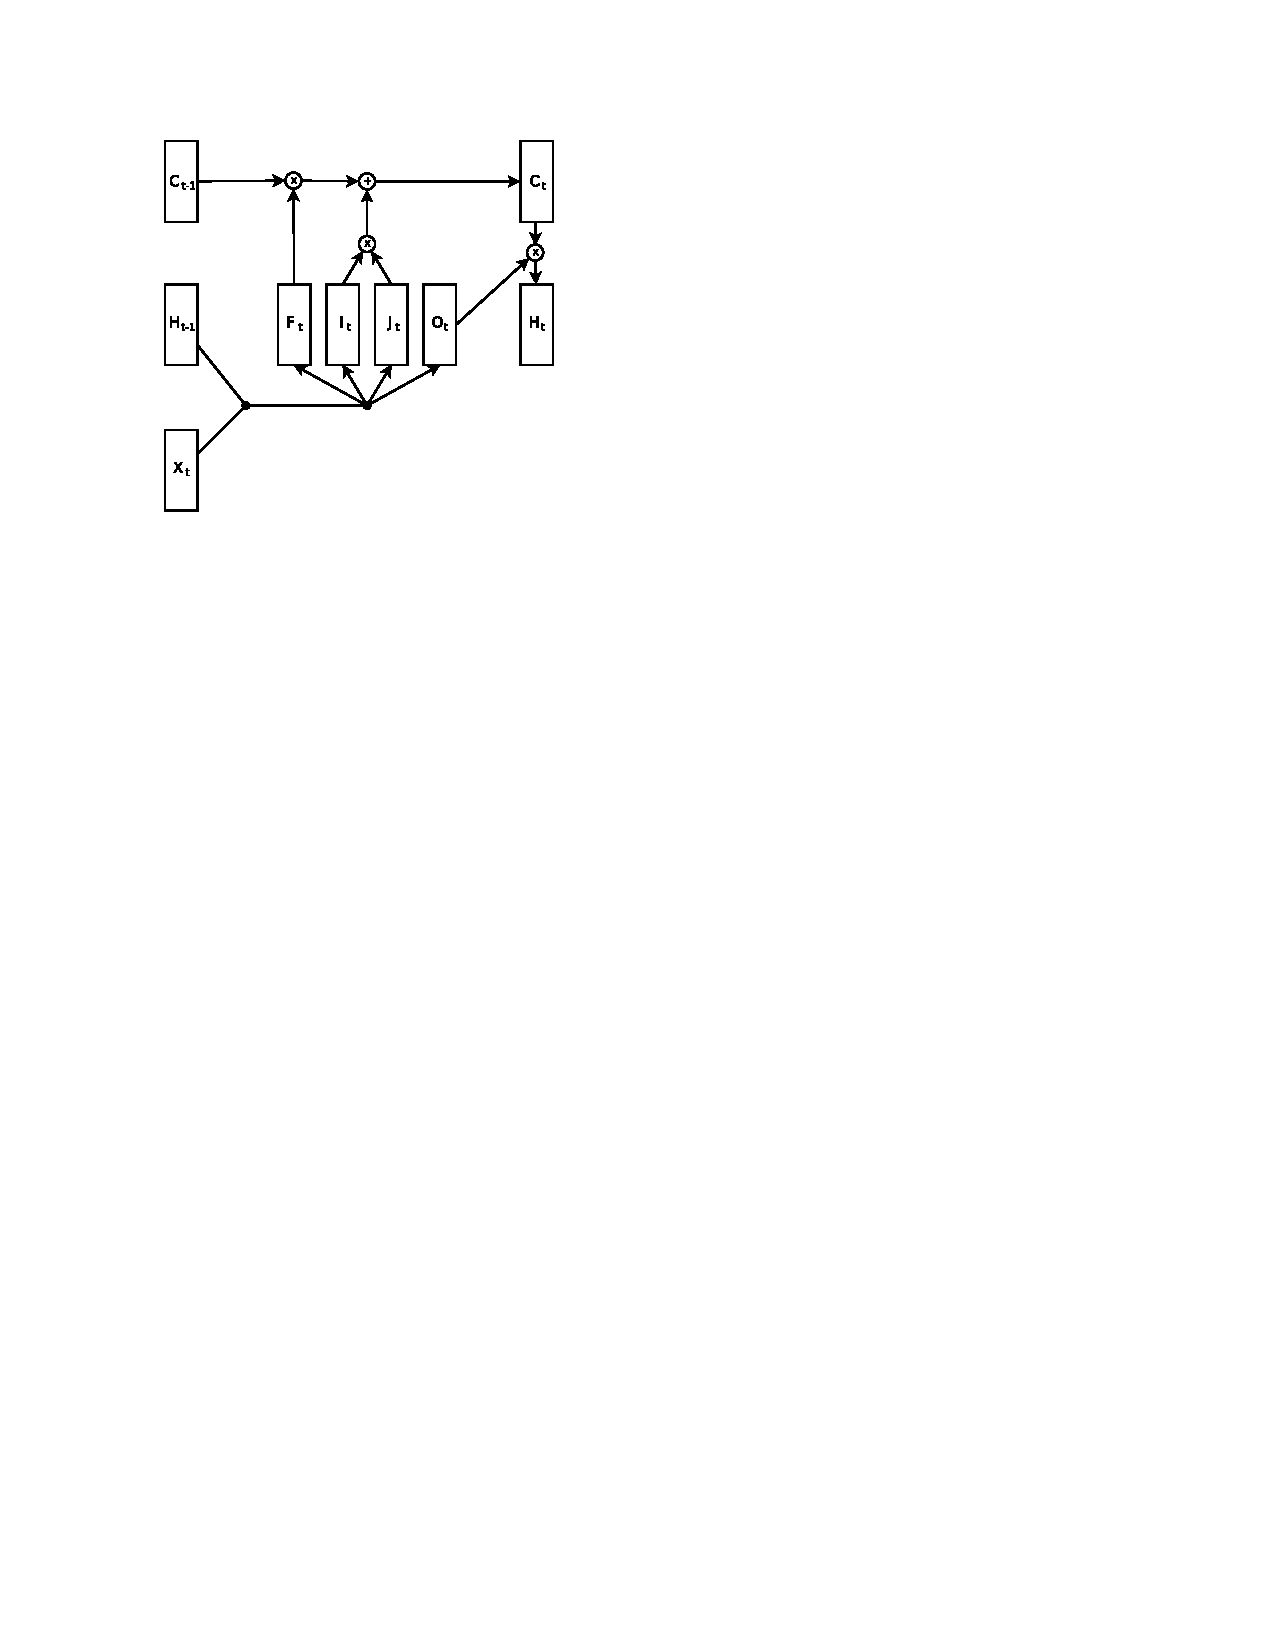
\includegraphics[width=0.7\columnwidth]{figures/methods/LSTM}
\caption{Long Short-term Memory. Source of figure: \cite{jozefowicz2015empirical}.}
\label{fig:methods:LSTM}
\end{figure}

The structure of LSTM is shown in Figure~\ref{fig:methods:LSTM}. The use of the gates is to allow the corresponding projection keep the original signal without applying any non-linearity, enabling part of the model to perform an identity mapping. Similar idea is recently applied to normal neural network by introducing ``residual connection", which is basically an identity mapping in addition to the original non-linear transformation. This significantly improved the performance of very deep neural netowrks (as deep as a thousand layers), related works can be found in \cite{srivastava2015highway, he2015deep, huang2016deep}.


\subsection{Paragraph Vector}
\label{section:paragraph_vector}
Using recurrent neural network is only one of the methods of sequence modeling. There are other methods which try to extend word2vec to phrase and sentence level. Given a vector representation of words, the most direct way of representing a sentence is taking the average of the corresponding word vectors. But this is obviously too simple, for the following reasons:

\begin{itemize}
    \item The words in a sentence should not be treated with equal attention. Different words are of different significance to the semantics of the sentence, hence in making the sentence representation, we should not use the same weight for all the words.
    \item The word order information is lost in this simple representation. Note that with the same set of words, different orders can render completely different meanings.
\end{itemize}

One way of making a better sentence representation is to leverage the parsing tree. In\cite{socher2011parsing}, the authors used a recursive neural network to process the parsing tree and build up the sentence representation along the tree structure. However this approach only works for sentences with good grammar because the final vector representation relies highly on the quality of the parsing tree.

In \cite{le2014distributed}, the authors proposed a much less complicated method which is a simple extension to the two models from word2vec, called paragraph vector. We will introduce the two extended models in the following.

\subsubsection{PV-DM}

\begin{figure}
\centering
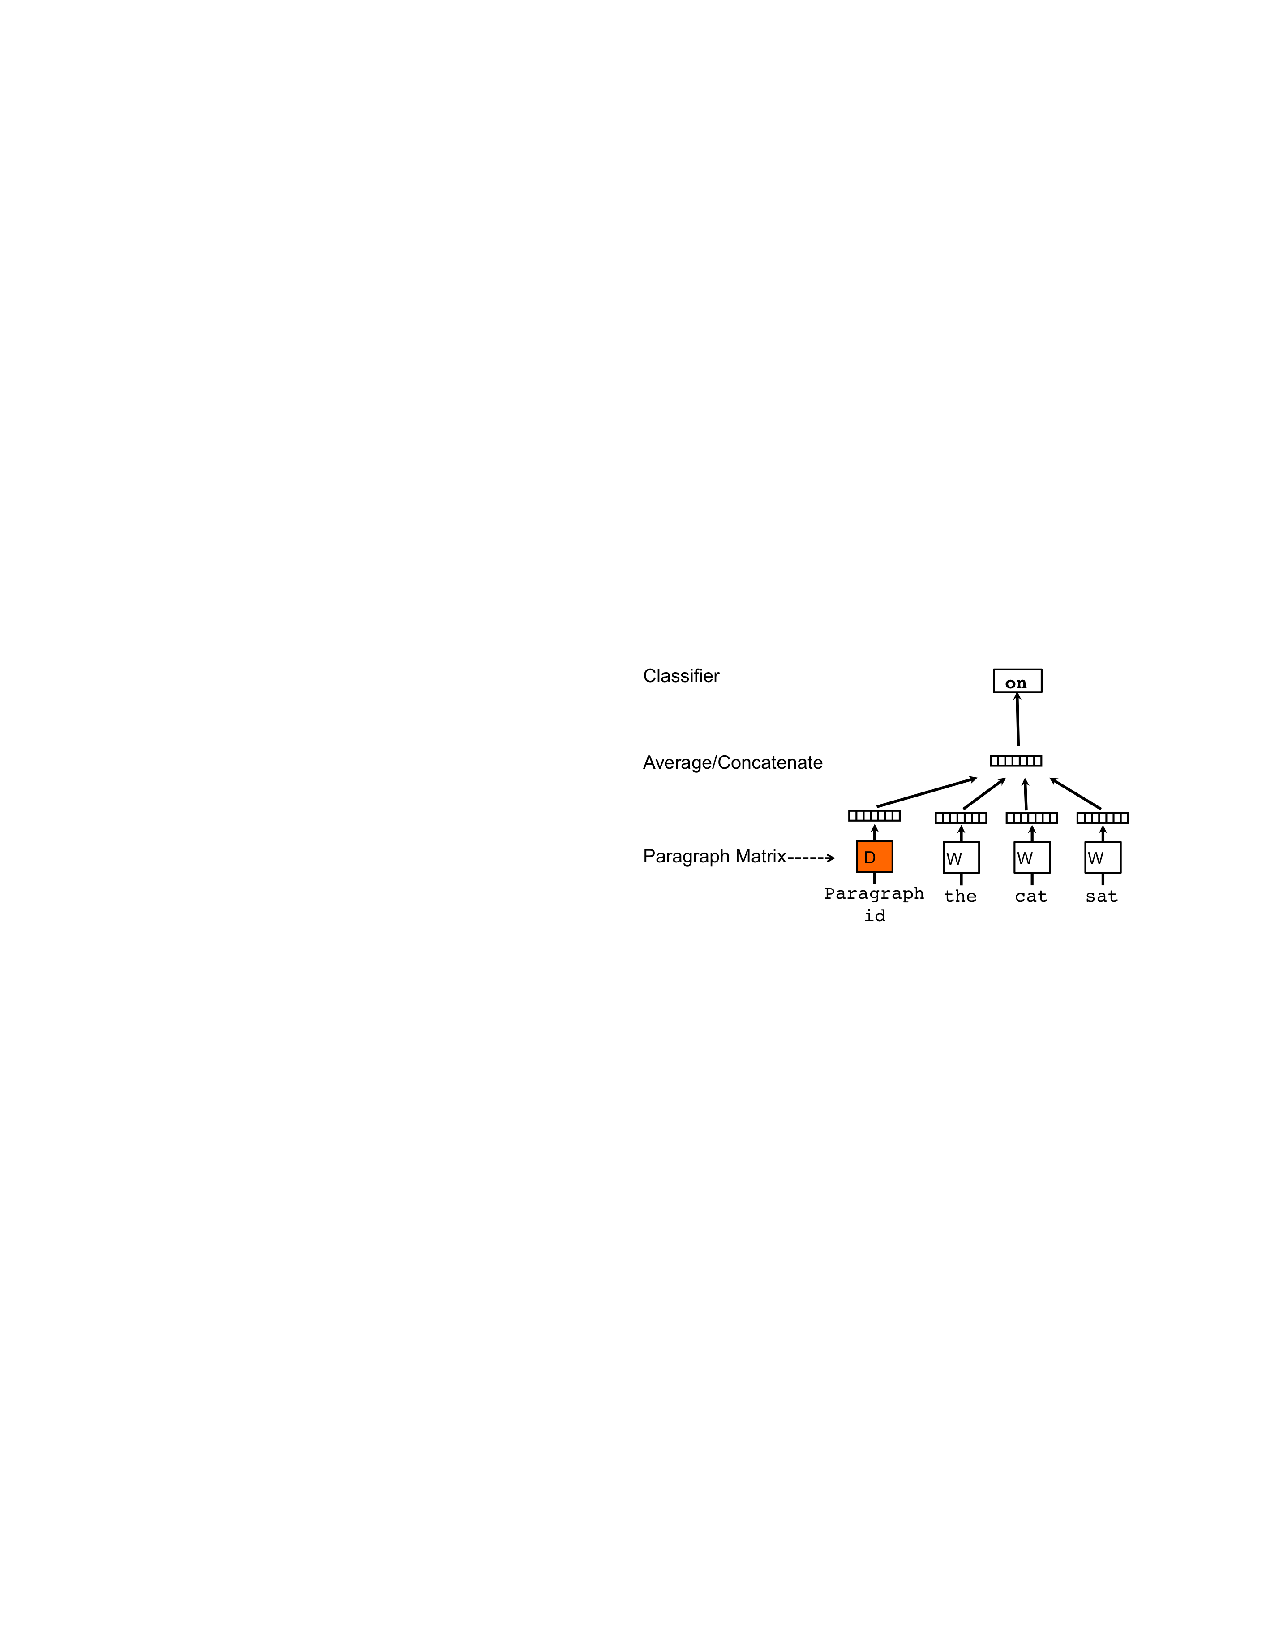
\includegraphics[width=0.5\columnwidth]{figures/methods/PV-DM}
\caption{The distributed memory model for paragraph vector.}
\label{fig:methods:PV-DM}
\end{figure}

In the previous section, we introduced one of the two models in word2vec, skip-gram. In skip-gram, one single word is used to predict every other word in the sentence, so that through back-propagation, the semantics of all other words is embedded in the word representation, resulting in a semantic embedding. In PV-DM (distributed memory for paragraph vector), a similar idea is adopted - a single paragraph vector is used to predict every word in the paragraph, so it can capture the semantics of all the words. Concretely, the model is defined by the following network structure, as shown in Figure~\ref{fig:methods:PV-DM}:

\begin{itemize}
    \item Each word in the dictionary is mapped to a word vector which is shared across all the sentence, just like word2vec. We can use pre-trained word vectors and fix them when training the paragraph vectors, or we can train the two representations simultaneously.
    \item Each paragraph is mapped to a vector (not necessarily in the same space with the word vectors), which is then passed through a feed-forward neural network, followed by a softmax output layer, just like skip-gram.
    \item The network predicts each word in the paragraph, with an opitimization objective of the log-likelihood of the whole corpus.
\end{itemize}

The only difference from skip-gram is that the word vector used for prediction is replaced with a pargraph vector.

\subsubsection{PV-DBOW}

\begin{figure}
\centering
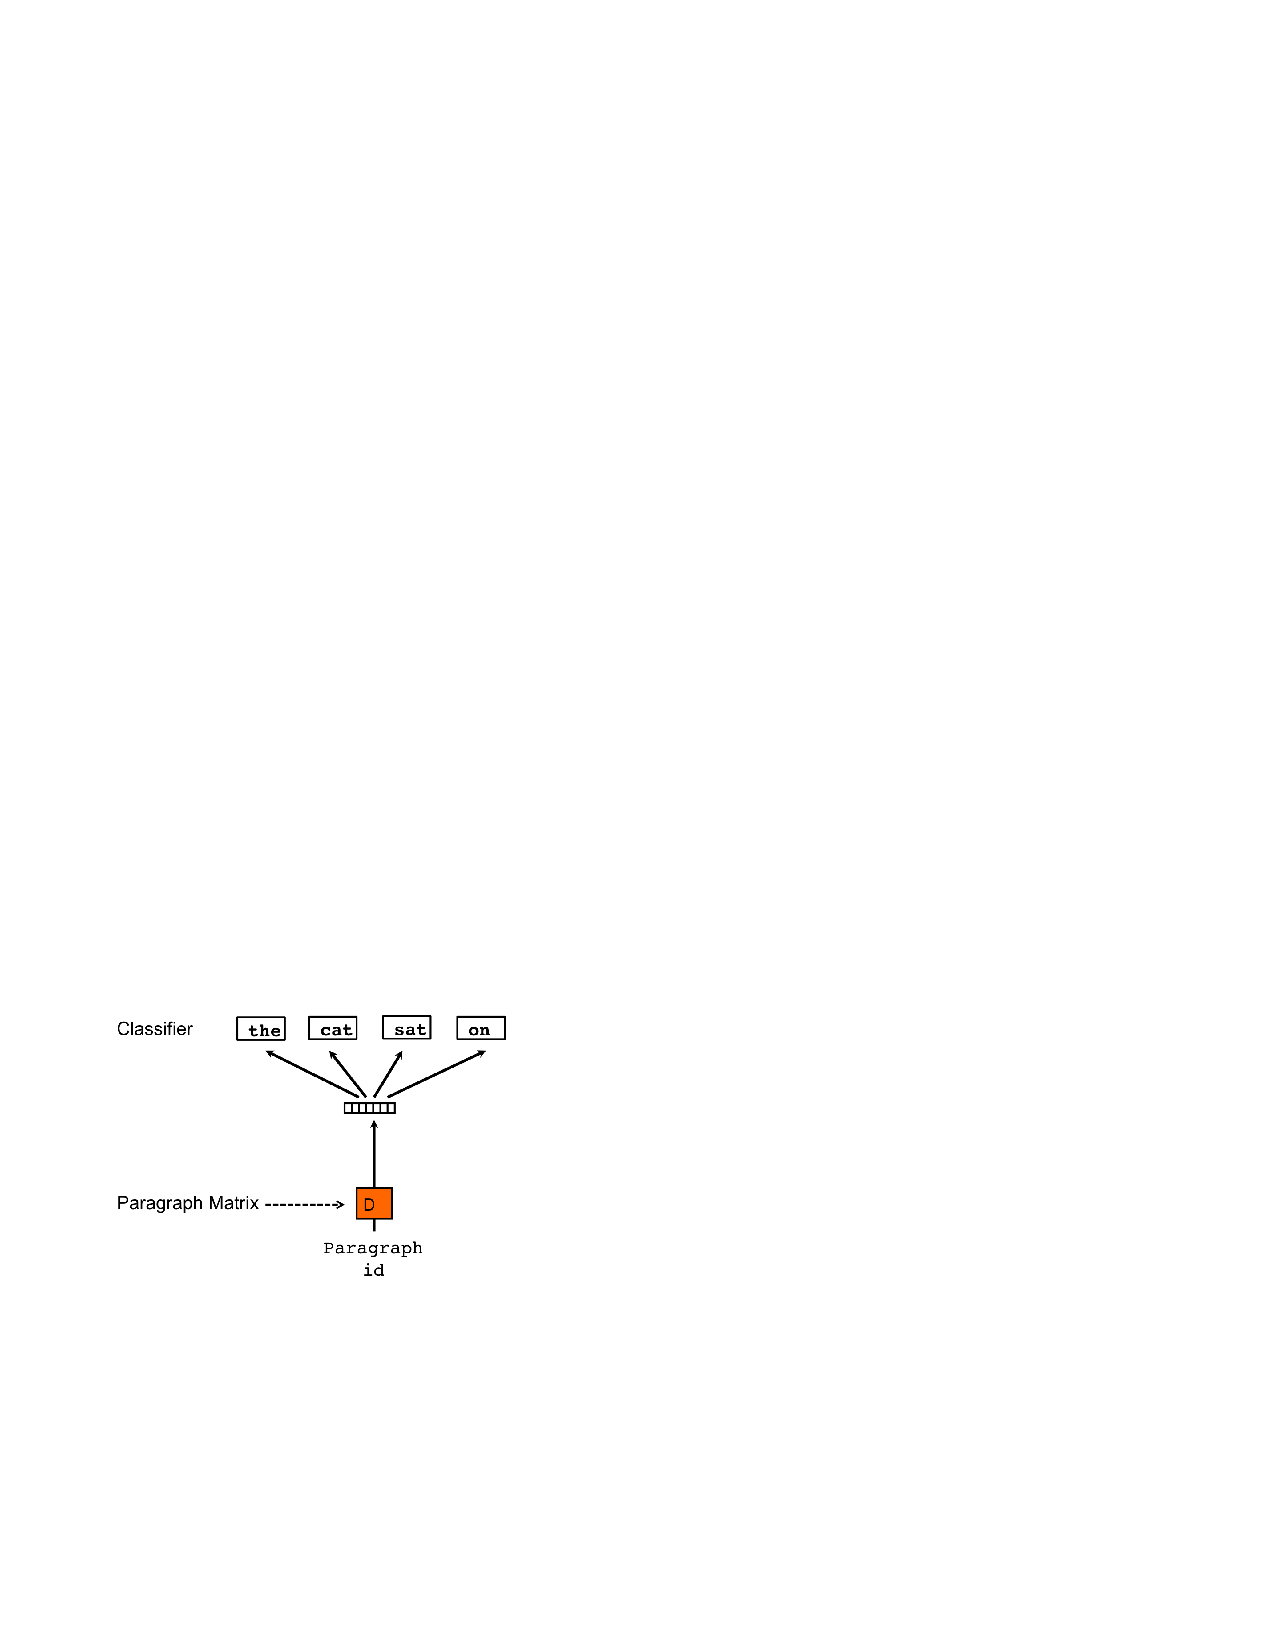
\includegraphics[width=0.5\columnwidth]{figures/methods/PV-DBOW}
\caption{The distributed bag-of-word model for paragraph vector.}
\label{fig:methods:PV-DBOW}
\end{figure}

PV-DBOW, or distributed bag-of-word for paragraph vector, is an extension to CBOW, continuous bag-of-word from word2vec. CBOW is defined by a n-gram neural network language model:

\begin{itemize}
    \item Each word is mapped to a vector.
    \item $n$ consecutive word vectors are concatenated together, fed through a feed-forward neural network and a softmax output layer to predict the next word in the sequence.
    \item The objective is the log-likelihodd of the whole corpus.
\end{itemize}

DBOW extends CBOW by using an extra paragraph vector, that is, in addition to the $n$ word vectors that are used to predict the next word, there is also a vector that represents the whole sentence, all concatenated together.The structure of PV-DBOW is shown in Figure~\ref{fig:methods:PV-DBOW}.

The final paragraph vector is the concatenation of the two vectors learned from PV-DM and PV-DBOW repectively and seperately.

\subsubsection{Advantages}

An important advantage of paragraph vector models is that they require no labeled data. Also, it doesn't require human experts to assign weights for words in a paragraph based on linguistic knowledge. The learned vector representations inherit an important property of word2vec, that is the semantics similarity. Also the final paragraph vector captures the word order information with the part learned from PV-DBOW with the n-gram model.

An advantage of paragraph vector over RNNs in practice is that it can leverage trained word vectors. The word vectors can be trained on a much larger corpus so they capture the semantics relationships more accurately, then the paragraph vecotrs can be trained on a relatively small dataset. Paragraph vectors are reported to word well with pre-trained word vectors. However, people find that it is more suitable to train the word vectors simultaneuosly for RNNs, so RNNs cannot leverage the word vectors learned from a larger dataset. Also, the paragraph vector models are simple and don't require storing a lot of information, by comparison for RNN we need to store every state during the forward pass for back-propagation, which is very memory consuming.

\chapter{Multistage Clustering Framework}

In this chapter, we introduce our proposed method for solving aspect extraction, a multistage clustering framework. We will first define the input and output of our model, then introduce the framework step by step.

\section{Problem Definition}

The problem we try to solve is unsupervised aspect extraction. The input is a corpus of reviews. The copurs consists of many reviews, and each review consists of several sentences. From this corpus we determine $K$ best aspects, each aspect $A_i$ being a set of candidate words $A_i = \{a_{i,j}\}$, which are typically nouns that are closely related to this aspect.

Note that in a run of our method, we only use a corpus of one domain to generate the aspects of that domain, without any information from other domains. This simplicity of the task allow our model to be applied to any domain.

\section{System Overview}

Our system takes as input the corpus of reviews about a product and outputs the $K$ best aspect words. The whole procedure consists of 2 parts: first we group the words related to potential aspects into clusters, then we select the best word from each cluster.

Our system consists of two main phases: clustering and ranking. In the first phase, we use a multistage clustering method, starting from a corpus of reviews, cluster at sentence level and evantually end up at word level. The result is a soft clustering of all the words appearing in the corpus - similar to topic modeling - each word appears in all the aspect clusters with different weights.

\begin{table}[t]
\centering
\begin{tabular}{|l|l|} \hline
Aspect & Words \\
\hline 
food & breakfast, meal, \textbf{food}, tasty, dinner, ... \\
\hline
staff & \textbf{staff}, desk, service, friendly, reception, ... \\
\hline
location & close, city, \textbf{location}, place, central, ... \\
\hline
room & bed, shower, spacious, \textbf{room}, size, ... \\
\hline
\end{tabular}
\caption{Result of clustering phase on hotel reviews. 
  Each row shows the candidate words of an aspect, sorted by the weight of each word. 
Bold-fonted words are the correct representatives of each aspect cluster.}
\label{table:cluster_example}
\end{table}

Table~\ref{table:cluster_example} shows an example of a real-life result of the clustering phase. Each row shows the candidate words of an aspect, sorted by the weight of each word. We only show the top words but each aspect actually contains all the words appearing in the corpus. The bold-fonted words are the correct representatives of each aspect cluster. In can be seen, not all of them are correctly sorted to be the top position. This is because the clustering phase is mainly based on co-occurrence of words, not the meaning of them. The sorting result of clustering can not fully capture the words' ability to represent or summarize the whole cluster. This motivates the second, ranking phase, which leverages knowledge bases to better measure the semantics of words.

In the following sections, we will introduce our clustering and ranking phases step by step.

\section{3-stage Clustering}

For clustering, we start with sentence vectors and go through 3 stages:

\begin{itemize}
	\item[1.] \textbf{Parallel text segmentation \& aggregation}

		By clustering the sentence vectors into $N$ clusters, we actually break each review documents into a few, each related one potential aspect.

	\item[2.] \textbf{Infer potential aspects}

		Recognize what are the potential aspects with Topic Modeling. From each cluster generate $M$ topics, in total $N\times M$ topics.

	\item[3.] \textbf{Resolve overlapping}

		Resolve the overlapping between aspect candidate clusters, remove noise from each cluster. Result in $C$ clusters.
\end{itemize}

With the $C$ final clusters, we want to find the $K$ best aspects. For this we go through a ranking system, which consists of 2 procedures:


% In the ranking process, we first rank the clusters on their quality. The better quality cluster ranks higher. Then we rank each cluster in the order we just got, that is, we first sort the cluster with better quality. We rank the words on how they summarize the whole cluster while considering the mutual information between the current one and the better quality, already sorted clusters.


\begin{itemize}
	\item[1.] \textbf{Rank clusters by quality}

		Rank the clusters by \emph{distinctiveness}, a metric for the quality of the cluster.

	\item[2.] \textbf{Rank words on their summarization ability}

		Score the words in each cluster on how well they summarize the whole cluster.
\end{itemize}

In the rest of the section, we introduce our approach step by step.

\subsection{Potential Aspect Clustering}
% In the first clustering procedure, we coarsely cluster the sentence vectors. We run a K-Means on the vector space and result $N$ clusters, each consists of sentences. Then we break each review documents by grouping the sentences by the clusters they are in. After this process, we result in $N$ clusters of documents. But now each document is only about topics related to one potential aspect.

As mentioned in previous chapters, one feature of review texts is that many topics are compressed into a short length where each of the topics might correspond to a potential aspect. sentences in a review that are close to each other may talk about completely different aspects about the product. Also sentences about the same aspect may not appear in the review in consecutive order. In order to perform topic modeling within the text about a single aspect, we need to group the sentences about the same aspect. This naturally leads to the segmentation of the text, which should to break a review into segments, each about a single aspect. 

For clustering sentences, we leverage paragraph vector introduced in Section~\ref{section:paragraph_vector}, which captures the semantic similarity between sentences.
We run the training of paragraph vector on the whole corpus, resulting in a vector representation for each sentence.

Here we make a simple and reasonable assumption: each sentence talks about only one aspect. So we break down each review into sentences and do a clustering on them all. We run a K-Means on the sentence vectors and generate $N$ clusters of sentences. We break each review based on the clusters and aggregate the sentences from the same cluster into a new document. So we actually break each review into a few, each being a topic-coherent 


\subsection{Inference of Aspect Words}
The first clustering process grouped related texts together and is rather coarse, the resulting clusters may have non-negligible overlapping. The overlapping appears as noises in each cluster and we need to seperate them from the actual topic of the cluster. Also our expected results is at the word level and the first clustering is at the sentence level, so we apply topic modeling. 

Within each cluster, we have the reduced documents formed by sentences from about the same potential aspect. We run LDA within cluster, generating $M$ topics each. 

For each cluster in the $M$ topics, some are noise. These noise topics for this cluster are very likely the result of overlapping. So we need to cluster all the topics again.

\subsection{Resolution of Aspect Overlapping}
From the LDA within each cluster, we have in total $N\times M$ topics where each topic is a distribution of words. Suppose dictionary size is $Z$, then we have $N\times M$ vectors of dimension of $Z$. We run another K-Means in this vector space after performing dimensionality reduction like PCA. This gives us $C$ clusters, each consists of topics. We take the center of each cluster as a natural representation of it. 

It is because of the existence of noise topics from LDA that we keep $C$ clusters instead of $K$, which the expected number of aspects. For our system to be fault-tolerant, we take more clusters than expected and cut out the noise by the following ranking process.


\section{Ranking}

The ranking phase takes the soft clustering by the previous phase and re-ranks both the clusters and the words in each cluster.

Note that the clusters by previous phase don't have an order. But in real life product reviewing, the aspects should be treated differently, the ranking of the aspects should reflect the opinion of the users. Also the quality of the clusters - how related are the words to the aspect - may vary, due to different frequencies of the aspects in the corpus. Also, the clustering is mainly based on co-occurrence of words, which may not fully capture the semantic relatedness of words. Motivated by these, we proposed to do a 2-stage ranking based on the clustering result, with the help of knowledge bases: first rank the aspect clusters, then the words in each cluster.

\subsection{Ranking Clusters}

We rank the clusters based on their quality. As analyzed in the previous section, the noise in each cluster is introduced by the overlap between clusters. We follow this direction and propose a measurement for the quality of clusters.

Our measurement is the \textbf{distinctiveness} of a cluster, namely how different is a cluster's word distribution from other clusters'. Intuitively, a cluster is of high quality when it has small overlapping with other clusters. We measure this by calculating the weighted sum of mutual information of the adjectives against all other clusters.

The mutual information of two random variables is a measure for the mutual dependence. For random variables $X$ and $Y$, their mutual information is defined by 
$$I(X, Y) = \sum_{y\in Y} \sum_{x\in X} p(x, y) \log\left(\frac{p(x, y)}{p(x)p(y)}\right)$$

In sorting clusters, we only consider the adjectives. Since aspect words are most likely to be nouns and our purpose of the clustering phase is to seperate them, they tend to be distinctive among clusters. Thus adjectives are more evenly distributed among clusters and can be used as a better measurement.

Let $a$ be any adjective in cluster $c, c\in[1,C]$ with frequency $f_c(a)$. Let $S(c, a)$ be the score of word $a$ in cluster $c$, then the score of the cluster $c$, $S(c) = \sum_{a} S(c,a)$. $S(c,a)$ is calculated by the mutual information between $a$ appearence in cluster $c$ and $a$ in all other clusters.

\begin{align*}
	S(c, a) &= \log\left(\frac{f_c(a)}{\sum_{r\in[1, C], r\neq c} f_r(a)}\right) \\
			&= \log(f_c(a)) - \log(\sum_{r\in[1, C], r\neq c} f_r(a))
\end{align*}

The score of each cluster is then calculated by the sum of scores of its adjectives. Finally the clusters are ranked in decending order of the score, implying the order of quality, from better to worse.

\subsection{Ranking Words}

Each cluster consists of words related to a potential aspect and we want to find what is the aspect. We do this by finding the word that best summarizes each cluster. For ranking the words in one cluster on how they summarize the cluster, we leverage the intuition behind Lesk lemmatization algorithm and a knowledge base WordNet to define a \emph{semantic similarity} $\sims(w_1, w_2)$ between words $w_1$ and $w_2$.
The semantic similarity measures how much the two words are related. The similarity consists of two parts:

\begin{itemize}
    \item Path similarty $\sims_p$ is calculated by the shortest path that connects two words in the is-a (hypernym/hyponym) taxonomy. The scores range from 0 to 1.
    \item Definition overlap $\sims_d$ is calculated based on the definition paragraphs of the two words. We train a recurrent neural network language model on a large dataset and use it to embed the paragraphs, then calculate the cosine of the two embedding vectors as the similarity of of the two definitions.
\end{itemize}

The final semantic similarity score is calculated by $\sims(w_1, w_2) = \sims_p(w_1, w_2) + \sims_d(w_1, w_2)$. When ranking words inside each cluster, we start with the clusters with high confidence, by the order calculated from the previous step. For word $w$ in cluster $i$, there is a weight, $u_{w,i}$, assigned by the LDA. When calculating the score of word $w$ in cluster $i$, denoted by $s_{w,i}$, we also consider its score from all previous clusters $1\sim i-1$, $s_{w,1} \sim {w,i-1}$. Similar to cluster ranking, we consider the mutual information, resulting in the final calculation of the score:
$$s_{w,i} = u_{w,i} \sum_{w'} \sims(w, w') - \sum_{j=1}^{i-1} s_{w,j}$$

The final word order in each cluster is sorted by this score.

\section{Experiments}

\label{sec:experiment}

%\begin{table*}[th!]
%   \centering
%   \scriptsize
%   \begin{tabular}{l|llcc}
%       \toprule
%       \textbf{Dataset} &\textbf{Premise}  & \textbf{Choices} & \textbf{Training size} & \textbf{Test size}\\
%       \midrule
%       \multirow{4}{*}{ROC} & Sarah was home alone. &\multirow{2}{*}{Sarah then happily watched the show.     %\checksymbol}&\multirow{4}{*}{1871}&\multirow{4}{*}{1871}\\
%                       &She wanted to stay busy. &     \multirow{2}{*}{Sarah could not find anything to watch. \crosssymbol } \\
%                       &She turned on the TV. \\
%                       &She found a reality show to watch.\\
%       \midrule
%       \multirow{3}{*}{ARCT} &\textbf{Reason}: Milk isn’t a gateway drug even though &\textbf{Warrant 1}: Milk is similar to marijuana. \checksymbol&\multirow{3}{*}{1210}&\multirow{3}{*}{444}\\
%       &most people drink it as children. &\textbf{Warrant 2}: Milk is not marijuana.\crosssymbol \\
%       &\textbf{Claim}: Marijuana is not a gateway drug. \\
%       \midrule
%       \multirow{4}{*}{RECLOR} &\textbf{Context}:In a business...to financial prosperity. &A: ignores the fact that in... the family 's prosperity.\checksymbol&\multirow{4}{*}{4638}&\multirow{4}{*}{500}\\
%       &\textbf{Question}:The reasoning in the argument&B: presumes, without... the family's prosperity.\crosssymbol&\\
%       & is flawed because the argument&C: ignores the fact... even if they pay high wages.\crosssymbol\\
%       &&D: presumes, without providing...can succeed.\crosssymbol\\
        
        
%       \bottomrule
%   \end{tabular}
%   \label{table:dataset}
%\end{table*}

%\begin{table*}[th!]
%    \centering
%    \scriptsize
%    \begin{tabular}{l|llcc}
%        \toprule
%        \textbf{Dataset} &\textbf{Premise}  & \textbf{Choices} & \textbf{Training size} & \textbf{Test size}\\
%        \midrule
%        \makecell[c]{COPA} &  \makecell[l]{I pushed the door.} &\makecell[l]{The door opened.     \checksymbol 
%        \\The door locked. \crosssymbol }&\makecell[c]{500}&\makecell[c]{500}\\
%        \midrule
%        \makecell[c]{ROC} &  \makecell[l]{Sarah was home alone.\\She wanted to stay busy.\\She turned on the TV.\\She found a reality show to watch.} &\makecell[l]{Sarah then happily watched the show.     \checksymbol 
%        \\Sarah could not find anything to watch. \crosssymbol }&\makecell[c]{1871}&\makecell[c]{1871}\\
%        \midrule
%        \makecell[c]{ARCT} &\makecell[l]{\textbf{Reason}: Milk isn’t a gateway drug even though \\ most people drink it as children. \\\textbf{Claim}: Marijuana is not a gateway drug.}&\makecell[l]{\textbf{Warrant 1}: Milk is similar to marijuana. \checksymbol \\
%        \textbf{Warrant 2}: Milk is not marijuana.\crosssymbol}&\makecell[c]{1210}&\makecell[c]{444}\\
%        \midrule
%        \makecell[c]{RECLOR} &\makecell[l]{\textbf{Context}:In a business...to financial prosperity. \\
%        \textbf{Question}:The reasoning in the argument\\  is flawed because the argument}&\makecell[l]{A: ignores the fact that in... the family 's prosperity.\checksymbol
%        \\B: presumes, without... the family's prosperity.\crosssymbol
%        \\C: ignores the fact... even if they pay high wages.\crosssymbol
%        \\D: presumes, without providing...can succeed.\crosssymbol}&\makecell[c]{4638}&\makecell[c]{500}\\
%        
%        
%        \bottomrule
%    \end{tabular}
%    \caption{Examples for all 4 datasets considered in this paper.}
%    \label{table:dataset}
%\end{table*}

\begin{table}[th!]
    \centering
    \scriptsize
    \begin{tabular}{l|ll}
        \toprule
        \textbf{Dataset} &\textbf{Premise}  & \textbf{Choices}\\
        \midrule
        \makecell[c]{COPA} &  \makecell[l]{I pushed the door.} &\makecell[l]{The door opened.     \checksymbol 
        \\The door locked. \crosssymbol }\\
        \midrule
        \makecell[c]{ROC} &  \makecell[l]{Sarah was home alone.\\She wanted to stay busy.\\She turned on the TV.\\She found a reality show to watch.} &\makecell[l]{Sarah then happily watched the show.     \checksymbol 
        \\Sarah could not find anything to watch. \crosssymbol }\\
        \midrule
        \makecell[c]{ARCT} &\makecell[l]{\textbf{Reason}: Milk isn’t a gateway drug \\
        even though most people drink it \\as children. \\\textbf{Claim}: Marijuana is not a gateway \\drug.}&\makecell[l]{\textbf{Warrant 1}: Milk is similar to marijuana. \checksymbol \\
        \textbf{Warrant 2}: Milk is not marijuana.\crosssymbol}\\
        \midrule
        \makecell[c]{RECLOR} &\makecell[l]{\textbf{Context}:In a business...to financial \\prosperity. \\
        \textbf{Question}:The reasoning in the \\argument is flawed because the \\argument}&\makecell[l]{A: ignores the fact that in... the family 's prosperity.\checksymbol
        \\B: presumes, without... the family's prosperity.\crosssymbol
        \\C: ignores the fact... even if they pay high wages.\crosssymbol
        \\D: presumes, without providing...can succeed.\crosssymbol}\\
        
        
        \bottomrule
    \end{tabular}
    \caption{Examples for all 4 datasets considered in this paper.}
    \label{table:dataset}
\end{table}



%1. Re-evaluate the extent to which the model is exploiting short circuit after augmentation. Test it on the same sampled examples to see the improvement of the percentage of cases where model look at context.

We evaluate the effectiveness of the proposed augmentation methods on four popular 
natural language reasoning tasks.
Three transformer-based models are employed as the
main targets for our experiments. 
We first show the experimental setup. 
%Second, we compare several operators for testing short circuit problem and apply the best one to multiple models on diverse NL reasoning tasks.
Then, we compare different augmentation methods on three models by the 
end-to-end tests, which contain
the stress test and original test of the four datasets, and demonstrate
the advantage of crossover and mutation. 
After that, we apply choice-only tests on the same set of models compared in the
last step, to reconfirm that performance gain in the end-to-end tests is
due to the reduction of short-circuit problems.
%Third, we reconfirm the findings in the end-to-end evaluations
%through additional choice-only tests. 
%without data augmentation 
%and of different modelswith choice-only test and 
Finally, we use a case study to discover the reason for the model improvement 
by the white-box test. 
%Finally we give a discussion about mutation augmentation method.

\subsection{Experimental Setup} 
\label{sec:setup}
% In this section, we will show our setup for datasets, models and test operators.
\subsubsection{Datasets}
We experiment on 4 datasets from four different tasks:
%\KZ{I think you need to say what is the context and what are the
%choices for these four datasets.}

\textbf{ROC} is a story ending prediction dataset. 
The task is to identify the correct ending of a four-sentence 
story premise from two alternative choices. 

\textbf{COPA} is a causal reasoning dataset, an example is previously shown
in~\secref{sec:intro}. Given a premise, 
COPA requires choosing the more plausible, causally related choice. 
%There are 500 instances in 
%training data and 500 instances for testing.

\textbf{ARCT} is an argument reasoning comprehension dataset. 
There may exist an alternative warrant choice 
in which the reason is connected to the claim.

\textbf{RECLOR} is a reading comprehension dataset that requires logical reasoning.

%Examples and statistics of them are shown in~\tabref{table:dataset}. 
Examples of them are shown in~\tabref{table:dataset}. 

%\begin{table}[th!]
%        \centering
%        \scriptsize
%        \begin{tabular}{l|l}
%                \toprule
%                \textbf{Oper.} &\textbf{Description and Example}\\
%                \hline
%                \multirow{3}{*}{Neg+} & Add negation (r$\rightarrow$w) \\
%                & Input: \textit{They called the police to come to my house. \checksymbol} \\
%                & Output: \textit{They {\textbf{{didn't}}}  called the police to come to my house. \crosssymbol} \\
%                \hline
%                \multirow{3}{*}{Neg-} &Remove negation (r$\rightarrow$w) \\
%                & Input: \textit{Ben {\textbf{never}} starts working out. \checksymbol} \\
%                & Output: \textit{Ben starts working out. \crosssymbol}\\
%                \hline
%
%                \multirow{3}{*}{NER} &Randomly replace person names (r$\rightarrow$w)\\
%                 & Input: \textit{A big wave knocked {\textbf{ Mary}} down . \checksymbol} \\
%                & Output: \textit{A big wave knocked {\textbf{ Kia}} down . \crosssymbol} \\
%                \hline
%                \multirow{3}{*}{PR} & Switch pronoun by gender or quantity (r$\rightarrow$w)\\
%        &Input: \textit{{\textbf{ She}} had a great time .\checksymbol} \\
%        &Output: \textit{{\textbf{ He}} had a great time . \crosssymbol} \\
%                \hline
%                \multirow{3}{*}{PI} &Instantiate pronoun by randome person (r$\rightarrow$w) \\
%        &Input: \textit{{\textbf{ They}} gave Tom a new latte with less ice . \checksymbol}\\
%        &Output: \textit{{\textbf{ Nathanael}} gave Tom a new latte with less ice . \crosssymbol}\\
%        \hline
%        \multirow{3}{*}{Voice} &Swap subject and object (r$\rightarrow$w) \\
%        & Input: \textit{{\textbf{Kara}} asked {\textbf{the neighbors}}  not to litter in their yard . \checksymbol} \\
%        & Output: \textit{{\textbf{the neighbors}} asked  {\textbf{Kara}}  not to litter in their yard . \crosssymbol}\\
%%               %\hline
%                %\multirow{3}{*}{Adv*} &Add adverbs for emphasis (w$\rightarrow$w)\\
%                %&Input: \textit{The ocean was as calm as a bathtub .\crosssymbol} \\
%                %&Output: \textit{{\textbf{ In fact}} the ocean was as calm as a bathtub .\crosssymbol} \\
%  %:ew              \hline
%              % \multirow{3}{*}{CO*} & Crossover: Swap the true choices between two questions (r$\rightarrow$w)\\ 
%        %&Input: \textit{\textbf{olive}Josh got sick . \checksymbol} \\
%        %&Output: \textit{\textbf{olive}{She had a great time .\crosssymbol}}  \\
%%\hline
% %               \multirow{3}{*}{Syn} &Replace adj/adv with synonym (w$\rightarrow$w) \\
% %               &Input: \textit{Dawn felt {\textbf{ happy}} about getting away with it . \crosssymbol} \\
% %               &Output: \textit{Dawn felt {\textbf{ glad}} about getting away with it . \crosssymbol} \\
%              % \multirow{3}{*}{MT*} & Mutate: Swap two consecutive words (r/w$\rightarrow$w) \\
%        %       & Input: \textit{Deb said yes {\textbf{olive} to} {\textbf{olive} Tim} 's marriage proposal. \crosssymbol} \\
%        %       & Output: \textit{Deb said yes {\textbf{olive} Tim} {\textbf{olive} to} 's marriage proposal .\crosssymbol} \\
%        %       & Input: \textit{Josh {\textbf{olive}got sick}. \checksymbol} \\
%        %       & Output: \textit{Josh {\textbf{olive} sick got}. \crosssymbol} \\
%          %     \hline
%
%                \bottomrule
%        \end{tabular}
%        \caption{Stress test operators considered in this paper.
%The first line in each cell describes the operation, the remaining lines in
%the cell give examples of how the operators work.
%r$\rightarrow$w indicates the operator turns a right choice into a wrong choice.}
%%while
%%w$\rightarrow$w indicates the operator turns a wrong choice into another wrong choice.}
%        \label{table:proxyop}
%\end{table}
%
%
\subsubsection{Stress Test Cases}
%Following previous research~\cite{checklist2020acl}, 
%we test the effectiveness of different data augmentation
%methods by looking at the robustness of models against
%different stress tests.
%We create these stress test cases using the operators
%in \tabref{table:proxyop}. Most of the operators
%have been proposed previously, except for PR and PI, which
%are newly introduced in this work.
%We create a stress test instance from a specific MCQ by 
%keeping the right choice and
%creating a \textbf{wrong} choice by applying one of the
%stress operators on the original right choice. This new
%wrong choice is \textit{grammatically correct}
%but \textit{logically incorrect} under the particular context. 
%Different operators generate different but sufficient number of cases 
%as shown in \tabref{tab:cases}.
%These stress test cases can evaluate not only the general model robustness, but also
%whether models are exploiting spurious features in the choices 
%rather than considering the connection between the premise and choices,
%or in other words ``short-circuiting.'' 
%
\begin{table}[th]
\centering
\scriptsize
\begin{tabular}{c|rrrr}
\toprule
\textbf{Stress} & \textbf{ROC} & \textbf{COPA} & \textbf{ARCT} & \textbf{RECLOR} \\ \midrule
Neg+  & 1,797&492&  297&375 \\ \hline
Neg-  & 94& 2&  152&    119\\ \hline
NER  &  362&    0&  5&0 \\ \hline
PR  &   1,073&  328&71&72   \\ \hline
PI  &        861&   219&    56& 91\\  \hline
Voice  &    1,014&246   &174    &263    \\  \midrule
%Adv  & 1,850&496   &444    &500    \\ \hline
%CO  &  1,871&500   &444    &500    \\ \hline
%Syn&   653&     25&    303&289 \\ \midrule
%MT  &  1,871&500   &444    &500    \\ \hline
Total &8,943    &2,287  &1,643  &1,920 \\ \bottomrule
%Total & 11,446  &  2,808 & 2,390 & 2,709 \\ \bottomrule
\end{tabular}
\caption{Number of stress test cases generated
by different operators for the four datasets.}
\label{tab:cases}
\end{table}

Different operators generate different but sufficient number of cases 
as shown in \tabref{tab:cases}.

To guarantee the correctness of questions in the stress test,
we sample 100 stress cases generated by each operation  
and annotate whether the cases are correct or not. The pass rate of these 
questions is mostly 100\% which indicates the 
reliability of these stress tests. However, there is only 
one special stress test, Neg+ test for COPA, 
with 94\% pass rate. Thus, we 
make extra human annotation to filter out incorrect data. The size of Neg+ 
stress test for COPA is changed from 492 to 463. It should be noted that 
all models are 
tested on the filtered stress test. 
For more details of human annotation, please refer to Appendix D.
%You may also wonder to know which kind of mutation is better. 
%If we believe mutation keeps its meaning and augment data with this operator, 
%although it can enhance fault tolerance of models, it does nothing for bias  
%elimination which is the main reason for model fragility in MCQ tasks. Because the 
%feature distribution based on different label is almost unchanged as the meaning.

%We evaluate the effectiveness and short circuits of all data augmentation methods 
%by the accuracy of the stress test set and the original test set.

%It should be noted that these stress tests are only used for robustness evaluation rather than 
%augmenting training data. Because some of the stress test operators 
%cannot generate a sufficient amount of data for training, like NER and Neg-. 
%Besides, we aim to design data augmentation methods to promote the model’s 
%general ability to avoid short-circuit, while most of the stress operators work 
%on a specific linguistic capability. 

%To evaluate the
%ability of testing for short-circuiting, we will
%use a subset of these test cases whose original MCQs are correctly answered by models in the next section.
%negation-add(Neg+),  negation-remove(Neg-), 
%NER, pronoun-replacement(PR), pronoun-instantiation(PI), 
%crossover(CO), adverbial(Adv), mutation(MT), Voice and synonym(Syn). 

% \footnotetext{The number denotes the number of questions 
% which can be transfered to a new stress test case with a certain operation.}
%we divide the stress test into two parts, the above part of~\tabref{table:tripleclassification} 
%are test types without syntax and  semantic errors, the following are test cases with errors.  
%compare different we re-evaluate the 
%exploiting short give the results
%on cue discovery as well as model probing along with some analysis. The whole framework has been implemented into
%an online demo at 
%review.

\subsubsection{Models}
We investigate three popular pre-trained language models: \textbf{BERT}, \textbf{RoBERTa}, and \textbf{XLNet}. 
To fine-tune the language models for an MCQ task, we feed LM's final hidden
vector to an MLP to compute the probability of the right choice.
We conduct all experiments on a server: 
a GeForce GTX 1080Ti GPU with 11G RAM and Intel(R) Xeon(R) CPU E5-2630 with 128G of RAM.

%\textbf{BERT} (BT) is a popular attention model, which applies the bidirectional training of Transformer. 
%%The basic one has 12-layer transformer, blocks, 768 hidden-size, and 12 self attention, 
%%heads, totally 110M parameters and fine-tune for 3 epochs to predict the relation based on context and 
%%choices.
%
%\textbf{XLNet} (XL) is trained with Permutation Language Modeling and without NSP.
%
%\textbf{RoBERTa} (RB) is an improved pre-training procedure of BERT.
%
Besides the original models (marked as w/o), we also train these three
models with four competing data augmentation methods: 
back-translation~\cite{back2019} (B),  crossover (C), mutation (M),
and the mixture of crossover and mutation with equal proportion (C+M). 
For each MCQ in the original training set, we create a new question using either one of
these 4 methods, yielding 4 augmented training sets the same size
as the original one.

We use back-translation as our baseline because it is 
popularly used in NLU tasks. While there exist promising data augmentation 
methods~\cite{qu2020coda,chen-etal-2021-hiddencut} that are based on dynamic perturbation of 
hidden states, back-translation is by far the most
effective data augmentation method that operates on the input level~\cite{kumar2020data}.
To this end, we generate a new question by conducting a round-trip English-to-French and 
French-to-English translation over each wrong choice. The translation model we utilized is mBART~\cite{liu2020multilingual}. 

Since crossover and mutation are operators for data augmentation, 
the modified questions do not need to be strictly correct. 
We also sampled 100 cases for each operator. 98\% and 97\% of the cases turned out
to be correct for \textit{crossover} and \textit{mutation}. 
% \KZ{Explain that why back-translation is the best
%baseline for data-only augmentation, and give some cites.}
%Other complicate data augmentation methods are hard to transform to all multiple-choice datasets. 
%\KZ{Do we need another stronger data aug baseline than backtranslation?
%since we are focusing on data aug now.} 

To ensure fairness, the training data augmented with +B, +C, +M, and +C+M are
all the same size. In +C+M, the extra data by +C and +M are equal in size. 
%The expanded data volume for each augmentation method is consistent with the original data volume.
%The expanded data volume is equal to the original data volume and 
%the size of new train dataset has doubled.

\iffalse
%\subsection{Testing for Short Circuit}
%\label{sec:short_circuit}
%In this section, we will select proper testing operators for short circuit testing and 
%we use these operators to detect the extent of model short circuit.

\subsubsection{Selecting Short Circuit Testing Methods}
\label{sec:select-sc}
%\KZ{Here we evaluate different black-box tests available to
%detect short-circuits in 3 different models. The ground truth
%is the attention map results generated by roy's code.}
%In~\secref{sec:proxy}, we have discussed the possibility that both white-box attention-based method and black-box choice operators 
%in some of the equivalent classes can evaluate short circuits. 
We now evaluate which proxy test operators are better suited for short circuit evaluation.
%For further exploring which operator is better for short circuit evaluation, 
%we sampled 100 random ROC questions that models had already done right for human annotation labeling. 
%Human annotators were asked to determine whether the model considered both premise and choice at the same time 
%with a visual attention map tool. 
%Different with AW,  human annotators are capable of reasoning, 
%and they do not consider relationships that have nothing to do with the answer, 
%such as punctuation and stop words between premise and choices. 
%As described in \secref{sec:proxy}, 
Each test operator generates new test cases by making directional changes to
the test cases that the model answers correctly. 
The model is considered not short-circuiting on a case according 
to a test operator if it still gets the right answer after the operation. 
%Assuming that human attention annotation, attention weight thresholding (AW), 
%and each choice operator are all plausible proxy tests, 

Including human attention annotation and choice-only test, we compare 8 different 
proxy tests in \tabref{tab:agree}. 
%In AW, the hyper parameter $t_1$ and $t_2$ are tuned to 0.14 and 0.13 separately 
We randomly sample 30 MCQs from the test set of ROC that are correctly answered 
by three models respectively. 
For each proxy test, we constructed a binary proxy vector 
of 30-dimensional one-hot vector~(proxy vector) for each model, where each dimension refers to 
a test case passing that proxy test (1) or not (0). If a model doesn't pass the proxy test 
on a certain test case, it means that model short-circuits on that specific MCQ. 
If a test case is not applicable to a proxy test, we generate 0 or 1 randomly.
%Each proxy test will produce a 30-dimensional one-hot vector~(proxy vector) for each model, where 1/0 indicates if the 
%model short-circuited on that specific MCQ or not. 
%\footnote{For MCQ where a certain proxy test is not applicable, we 
%randomly label it as 1 or 0.}. 
For each model, we then compute another vector as the ensemble of all proxy tests by 
majority voting on each of the 30 dimensions. We use the Euclidean distance between the 
proxy vector and the ensemble vector (i.e., center) because the test 
closest to the center will be the most 
representative and applicable to most test cases.  
%The scriptsizeer euclidean distance between the individual proxy vector of each test type 
%and the ensemble vector indicates higher reliability. 
We can find that the results of CO are generally closer to the ensembled results. 
Thus, we use CO as the proxy test for short circuit evaluation in the rest of
this section. 

\begin{table}[th]
    \scriptsize
    \centering
    \begin{tabular}{c|cccc}\hline
        \toprule  
        \textbf{Test types} &BERT  & XLNet & RoBERTa  &Ave\\ 
        \midrule
        {Neg+}      &  4.24     &   3.46  & \textbf{2.65}   &3.45\\
        \midrule
        {Neg-}&   4.0   &       3.61  & 3.87    &3.83\\
        \midrule
        {NER}    &   4.0    &  3.46      &  4.24    &3.9\\
        \midrule
        {PR}&    4.0    &    3.32   &   4.0 &3.77\\
        \midrule
        {PI}&   3.32    &    4.0    &   3.16    &3.49\\
        \midrule
        {CO}  &      \textbf{2.0}       &  \textbf{ 2.0} &  2.83    &\textbf{2.28}\\
        \midrule
        %{AW}   &  \textbf{2.45}    &3.46&  \textbf{2.45}   &\textbf{2.79} \\
        %\midrule
        {Choice-only}   &  4.12     &3.87  &    3.87    &3.95\\
        \midrule
        {Human}   & 2.24    &   3.0&    3.0 &2.75\\
        \bottomrule
        \hline
    \end{tabular}
    \caption{\label{tab:agree} 
        Euclidean distances between proxy vector and 
        the ensemble vector on short circuit test (the scriptsizeer
        the better). 
        Ave is the average score across all models.
        Top test type for each model are highlighted.}
\end{table}

It is noted that we choose not to use a higher-dimensional vector
here because a) we are not computing accuracy or
pass rate, so statistical significance
is not an issue, and b) in a 30-dimensional space,
we can already sufficiently distinguish these short
circuit tests in \tabref{tab:agree}. Adding more test cases
or more dimensions will not change that distinction.

In our experiment, we do not use human labeling results on the attention map 
as gold indicators.  Because the attention map on each model is not a direct 
expression of the final decision for multiple-choice questions, 
but the expression of the premise and choices which is an indirect information for reasoning.

\fi


%%\begin{table}[th]
%%\scriptsize
%%\centering
%%\begin{tabular}{c|cccc}\hline
%%\toprule  
%%\textbf{Test types} &BERT  & XLNet & RoBERTa  &Ave\\ 
%% \midrule
%%{Neg+}      &     30.06    &46.67&    19.55   &32.09\\
%%\midrule
%%{Neg-}&    47.22  &63.33& 64.52   &58.36\\
%%\midrule
%%{NER}    &    49.94   &46.67  &51.61  &49.41\\
%%\midrule
%%{PR}&      30.99  &43.33  &38.71& 37.68\\
%%\midrule
%%{PI}&    34.07    &40&    35.48   &36.52 \\
%%\midrule
%%{CO}            &     21.98   &23.33  &25.81  &\textbf{23.71}\\
%%\midrule
%%{AW}   &     22.28    &40&    19.35&  \textbf{27.21}\\
%%\midrule
%%{choice-only}   &     22.28   &40&    19.35&  \textbf{27.21}\\
%%\midrule
%%{Human}   &75.98  &20 &29.03  &41.67\\
%%\bottomrule
%%\hline
%%\end{tabular}
%%\caption{\label{tab:agree} Euclidean distance between test type vector and the ensemble vector on short circuit test. Ave is 
%%the average score across all models.}
%%\end{table}
%
%

%Each operator in~\table{tab:agree} are possible to show whether the model has short circuit problem to a certain extent, In order to choose a more appropriate method, we adopt the following strategies: find the focus of these methods, that is, vote on a topic. If most methods think that the model cheats on this topic, then this topic will be considered cheating. According to the various methods and the Euclidean distance of the selected answer, choose the method that is more suitable for short-circuit test

%\begin{table}[th]
%\scriptsize
%\centering
%\begin{tabular}{c|ccc}\hline
%\toprule  
%\textbf{Test types} &BERT (\%) & XLNet (\%) & RoBERTa (\%)  \\ 
% \midrule
%{Neg+}      &     36.67      &      47.83   & 52  \\
%\midrule
%{Neg-}&     50     &   60 & 40  \\
%\midrule
%{NER}    &     66.67       &    42.85          &   35.71\\
%\midrule
%{PR}&      47.61       &    44.44      &  26.31  \\
%\midrule
%{PI}&     50           &   50    & 35.71  \\
%\midrule
%{CO}            &     83.33        & \textbf{ 70}       &    70.97\\
%\midrule
%{AW}   &      \textbf{99.6}     & 66.67 &   \textbf{77.42} \\
%\bottomrule
%\hline
%\end{tabular}
%\caption{\label{tab:agree} The agreement on short circuit 
%detection between human annotation and each proxy test.}
%\end{table}
%
%\subsubsection{Testing Short Circuit Problems}
%\label{sec:fix-sc}
%%We test short circuits by observing AW and CO scores, 
%%i.e., higher AW/CO scores indicate a lower chance for short-circuiting. We fine-tune the multiple choice classifiers of BERT, XLNet and RoBERTa on 4 datasets. 
%Each number in ``Short Circuit Tests'' columns of
%\tabref{tab:results} denotes
%the percentage of test cases that pass 
%the proxy short circuit test. 
%The higher the percentage, the lower the possibility of short circuit problem.
%Each group of models (e.g., BT*) are tested
%on the subset of the original test set (1871 cases for ROC)
%that vanilla model answers correctly.
%For example, the test set for BT* on ROC contains 
%1871*86.58\% = 1620 questions.
%
%In~\tabref{tab:results}, we fine-tune the multiple-choice classifiers of BERT, XLNet and RoBERTa on 4 datasets 
%with their original training data. 
%We can find that all models trained on original data (in gray color) without 
%data augmentation generally suffer from lower short-circuit passing rates. 
%%We can find that the original models (the gray part in ``Short circuit Test'' column) without 
%%data augmentation are most likely to have short-circuits because the CO score are quite low. 
%%lower CO scores indicate a higher chance for short-circuiting. 
%Unsurprisingly, all models tend to short-circuit on COPA, 
%as it has been shown to contain easy-to-exploit 
%single-token cues by prior work~\citep{kavumba-etal-2019-choosing}. 
%RECLOR is a relatively hard task for models to solve as model 
%accuracies on the original test set are generally 
%lower than other tasks. 
%Nevertheless, the fairly low short circuit test passing rates indicate that these models are still largely making use of superficial cues in the datasets. 
%%Thus we can conclude that short circuit is a serious and common problem which is harmful for 
%%model robustness on different tasks.
%
%We further evaluate the augmented models (with white background in 
%``Short Circuit Tests'' columns) 
%using the short circuit test. According to \tabref{tab:results}, 
%models augmented by crossover always gets the highest short circuit test
%score. It indicates that model learns to reason jointly over both premise and choice. 
%Back-translation doesn't help ameliorate short circuit much, 
%possibly because cues being exploited are still kept after back-translation process. 
%Mutation turns out to be not as effective as crossover for alleviating short circuit. 
%This is likely due to mutation introducing incorrect syntax to the wrong choice, 
%which makes it easier to be eliminated by models.
%
%

%\KZ{Remove the parts about overall robustness} 


%\begin{table}[th!]
%   \centering
%   \scriptsize
%   \begin{tabular}{ll|cc|cc}
%       \toprule
%       \textbf{Dataset} &\textbf{Model}  & \textbf{AW} & \textbf{CO\_sc} & \textbf{Original}&\textbf{Stress}\\
%       \midrule
%       \multirow{3}{*}{ROC} & BT &98.76&90.80&86.58&81.93\\
%       &XL& 28.08&83.28&90.81&79.22\\
%       &RB&77.41&88.76&92.73&82.33\\
%       \cmidrule{2-6}
%       \multirow{3}{*}{COPA} & BT &89.68&68.71&62.00&57.40 \\
%       &XL& 93.16&60.26&61.40&57.71\\
%       &RB&80.89&78.01&76.40&74.85\\ \cmidrule{2-6}
%       
%       \multirow{3}{*}{ARCT} & BT & 9.65&78.52&63.96&58.08\\
%       &XL& 85.67&59.10&75.45&61.72\\
%       &RB&  99.14&60.29&78.83&66.16\\ \cmidrule{2-6}
%           
%       \multirow{3}{*}{RECLOR} & BT &    82.46&50.88&45.6&33.91\\
%       &XL&  79.64&62.86&56.0&39.77\\
%       &RB&85.88&70.2&51.0&36.76\\
%       \bottomrule
%   \end{tabular}
%   \caption{Evaluation models with short circuit test and robustness 
%   test on 4 different datasets. $CO_sc$ denotes we use crossover operator for short circuit evaluation}
%   \label{tab:original}
%\end{table}


%\KZ{Compare crossover, mutation, backtranslation's abilities to
%fix the short-circuit problems. Use roy's code to evaluate
%the new models after augmentation to show that short-circuit problems
%drops the most under crossover.}

%\subsubsection{Generating Augmented Data}
%We first apply the proposed two operators \textit{crossover}~(C) and \textit{mutation}~(M) as well as their combination \textit{crossover}+\textit{mutation}~(C+M) to generate additional training data. For each MCQ in the original training set, we follow the description in \secref{sec:crossover} and \secref{sec:mutate} 
%to generate one additional MCQ using C, M, or C+M. 
%
%
%
%The quantity of augmented data generated by each method is the same as the original training data of each dataset, giving rise to a fair comparison.
%
\subsection{End-to-end Test}
%\KZ{It's a little strange to have this as a section. More like part
%of implementation details?}
%To improve the diversity of augmented examples, 
%we explore back-translation and our \textit{crossover} and \textit{mutation} strategies.
In this subsection, we explore the capabilities of models with 
different data augmentation methods, i.e., back-translation, \textit{crossover}, and 
\textit{mutation}, from overall and fine-grained perspectives. 
The overall perspective shows the accuracy results from the stress test set and 
the overall original tests. Fine-grained perspective shows the stress test accuracy 
results by different stress operators. We train each model 3 times with different seeds and 
calculate their average score as the reusults of each test.  

%\KZ{No such thing as micro result}
%\begin{table*}[th]
%    \scriptsize
%    \centering
%        \begin{tabular}{l|cc|cc|cc|cc|cc}\toprule
%            \multirow{2}{*}{\textbf{Model}} & \multicolumn{2}{c|}{\bf ROC} & \multicolumn{2}{c|}{\bf COPA} & \multicolumn{2}{c|}{\bf ARCT} & \multicolumn{2}{c|}{\bf RELOR}& \multicolumn{2}{c}{\bf Average of 4 Datasets} \\ \cline{2-11}
%            & \textbf{Original} &\textbf{Stress}&\textbf{Original} &\textbf{Stress}&\textbf{Original} &\textbf{Stress}&\textbf{Original} &\textbf{Stress} & \textbf{Original} &\textbf{Stress} \\ \hline
%            %\rowcolor{gray}
%BT(w/o)&86.58&79.39 &62.00&55.64 &63.96&48.74 &45.60&22.83 &64.54 &51.65 \\
%BT+B&86.75&82.41 &68.60&68.64 &68.47&45.96 &48.60&24.94 &68.11 &55.49 \\
%BT+C&87.07&83.33 &72.80&80.86 &68.92&56.29 &47.00&49.89 &68.95 &67.59 \\
%BT+M&86.48&88.54 &70.40&81.63 &67.79&65.96 &46.80&46.08 &67.87 &70.55 \\
%BT+C+M&86.75&91.40 &72.40&82.80 &67.57&69.27 &43.60&53.14 &67.58 &74.16 \\
%            \midrule
%XL(w/o)&90.81&73.70 &61.40&52.61 &75.45&45.83 &56.00&24.93 &70.92 &49.27 \\
%XL+B&90.43&78.56 &63.20&63.89 &79.05&55.23 &57.00&33.37 &72.42 &57.76 \\
%XL+C&89.47&85.60 &67.80&76.26 &74.55&58.15 &54.40&48.87 &71.56 &67.22 \\
%XL+M&90.17&89.25 &62.20&72.61 &74.10&69.80 &53.60&54.55 &70.02 &71.55 \\
%XL+C+M&90.22&92.88 &67.20&87.00 &77.03&74.44 &54.20&56.47 &72.16 &77.70 \\
%            \midrule
%RB(w/o)&92.73&76.39 &76.40&74.94 &78.83&53.25 &50.40&18.25 &74.59 &55.71 \\
%RB+B&92.46&69.70 &77.00&81.94 &81.31&54.04 &51.00&22.03 &75.44 &56.93 \\
%RB+C&91.18&88.00 &79.00&84.36 &77.93&54.31 &50.40&51.91 &74.63 &69.64 \\
%RB+M&93.62&88.06 &72.60&88.17 &77.03&76.29 &52.00&60.53 &73.56 &78.27 \\
%RB+C+M&91.88&91.79 &74.00&93.46 &75.00&70.99 &48.40&55.77 &72.32 &78.00 \\
%            \bottomrule
%        \end{tabular}
%    \caption{\label{tab:results} Overall test
%        on 4 models with or without(w/o) data augmentation.
%        All numbers are percentages (\%). 
%        +B = augmented with back-translation,
%        +C = augmented with crossover, +M = augmented with mutation.
%The last two columns summarize the performance on 4 datasets.}
%    %Robustness Test includes: Neg+=negation-add, Neg-=negation-remove, NER, 
%    %PR=pronoun-replacement, PI=Pronoun-instantiation, Adv=adverbial, MT=mutation, Voice, Syn=synonym.}
%\end{table*}
%

\subsubsection{Overall results}
\label{sec:overview}

\begin{table}[th]
    \scriptsize
    \centering
        \begin{tabular}{l|c|c|c|c} \toprule
            \textbf{Model} &\bf{ROC} &\bf{COPA} & \bf{ARCT} & \bf{RELOR} \\ \midrule
            %\rowcolor{gray}
BT(w/o)&77.48 &62.55&33.07 &22.83 \\
BT+B&82.35 &77.47 &44.75 & 24.94\\
BT+C&85.35 &76.94 &53.87 & 49.89\\
BT+M&87.60 &82.19 &\textbf{71.82} &46.08 \\
BT+C+M&\textbf{91.31}&\textbf{86.83}&70.22 &\textbf{53.14} \\
%BT+B+C+M&\textbf{93.47}&83.97&69.64 &  \\
            \midrule
XL(w/o)&73.95 &62.47 &53.20 & 24.53\\
XL+B &75.30 &64.81 &54.00 & 33.37 \\
XL+C &85.38 &82.54 &60.71 & 48.87 \\
XL+M &88.02 &76.65 &69.73 & 54.55\\
XL+C+M & \textbf{92.35} &\textbf{91.38} &\textbf{73.07} & \textbf{56.47}\\
%XL+B+C+M & \textbf{93.44} &85.71 &72.98 & \\
            \midrule
RB(w/o)&77.58 &68.83 &49.20 &18.15\\
RB+B &76.17 &77.71 &53.38 & 22.03\\
RB+C &88.46 &91.45 &56.72 & 51.91\\
RB+M&88.55 &86.01 &73.33 & \textbf{60.53}\\
RB+C+M &\textbf{94.39} &\textbf{93.63} &\textbf{74.13} &55.77 \\
%RB+B+C+M &\textbf{94.90} &91.28 &73.02 & \\
            \bottomrule
        \end{tabular}
    \caption{\label{tab:stressresults} Overall stress test
        on 4 models with or without(w/o) data augmentation.
        All numbers are percentages (\%). 
        +B = augmented with back-translation,
        +C = augmented with crossover, +M = augmented with mutation.}
    %Robustness Test includes: Neg+=negation-add, Neg-=negation-remove, NER, 
    %PR=pronoun-replacement, PI=Pronoun-instantiation, Adv=adverbial, MT=mutation, Voice, Syn=synonym.}
\end{table}

\begin{table}[th]
    \scriptsize
    \centering
        \begin{tabular}{l|c|c|c|c} \toprule
            \textbf{Model} &\bf{ROC} &\bf{COPA} & \bf{ARCT} & \bf{RELOR} \\ \midrule
            %\rowcolor{gray}
BT(w/o)&88.49&64.60&61.94&45.60\\
BT+B&88.42&75.4&71.70&48.60\\
BT+C&87.60&75.73&70.80&47.00\\
BT+M&87.69&69.53&65.92&46.80\\
BT+C+M&87.47&73.2&68.54&43.60\\
%BT+B+C+M&\textbf{91.25}&73.27&66.36&\\
            \midrule
XL(w/o)&90.88&63.40&77.85&56.00\\
XL+B&90.88&64.80&77.70&57.00\\
XL+C&90.52&74.60 &78.60&54.40\\
XL+M&90.08&66.80&75.45&53.60\\
XL+C+M&90.40&72.93&76.95&54.20\\
%XL+B+C+M&\textbf{92.57}&72&76.27&\\
            \midrule
RB(w/o)&92.16&72.00&77.10&50.40\\
RB+B&92.16&74.07&80.93&51.00\\
RB+C&91.68&77.07&79.05&50.40\\
RB+M&91.91&70.47&78.23&52.00\\
RB+C+M&92.46&75.67&77.78& 48.40\\
%RB+B+C+M&\textbf{93.85}&75.73&76.80& \\
            \bottomrule
        \end{tabular}
    \caption{\label{tab:oriresults} Overall original test
        on 4 models with or without(w/o) data augmentation. %The best results for each dataset on each model
%are highlighted.
}
    %Robustness Test includes: Neg+=negation-add, Neg-=negation-remove, NER, 
    %PR=pronoun-replacement, PI=Pronoun-instantiation, Adv=adverbial, MT=mutation, Voice, Syn=synonym.}
\end{table}



%\KZ{Pls check the caption of all the tables and figures. Many of them
%are not right.}
%\textit{Crossover} and \textit{mutation} are both designed to teach models 
%to pay more attention to the relationship between the premise and the choices. 
%But they are quite different methods. \textit{Crossover} make the choices vary widely. 
%\textit{Mutation} makes the two choices of a question very similar except for the 
%order of the words. This forces the model to look to the premise to avoid short-circuit problems.

%The overall comparison results for \textit{crossover} and 
%\textit{mutation} are shown in \tabref{tab:stressresults} and \tabref{tab:oriresults} 
%which denote the percentage of cases in the stress and original test set 
%that is correctly predicted by the models. 

% For example, ROC has 1871 test cases~(\tabref{table:dataset}).
% The scores in the ``Stress'' columns are the percentage of
%Note that in the last two columns,
%we average the accuracies over the four datasets, because they are equally 
%important to us.  This approach is similar to the macro-average used in 
%the evaluation of classifications.  

%It's noted that these four datasets all have 
%a sufficient number of test cases to be statistically significant.

%\KZ{Compared with w/o and +B, we do well with stress tests. That's no
%problem. But with original, things are not that clear. We (including
%+C and +M and +CM) are better than w/o in 8/12 cases, better than +B
%in 7/12 cases. So the success is not overwhelming. Maybe we need to
%compute the average F1 over all the datasets for each model, or
%even the average of all the cases to make us look better?
%We need to discuss how to present it to make it look good.}
In~\tabref{tab:stressresults} and \tabref{tab:oriresults}, we can find 
that vanilla BERT, XLNet, and RoBERTa 
are mostly not robust on stress tests across all datasets.
Compared to the original test data, 
the accuracy on the stress tests has dropped substantially for models 
without data augmentation. 
For example, BERT (w/o) model on ROC task achieves 88.49 \% accuracy result (in \tabref{tab:oriresults}) 
but only achieves 77.48 \% (in \tabref{tab:stressresults}) which drops by about 11\%.
On average, the accuracy drops by 16.21\% for BERT (w/o), 12.04\% for XLNet (w/o) 
and 19.54\% for RoBERTa (w/o). 
%Similarly, all three models perform much 
%worse than before on COPA (-8.79\%), ROC (-17.11\%), and ARCT (-29.62\%). 
It confirms that the original models are fragile with short-circuits and 
can be confused by questions that require a stronger connection between the premise
and the choice. 
%Furthermore, there are two possible sources for model fragility: 
%model structure and spurious features in training data. 
%Since the model is black-box and hard to interpret, 
%we explore the source from the data. 
%\KZ{If the model can get better performance on stress tests with a 
%data augmentation method, it suggests that the source for model fragility
%is from the data instead of the model structure.} 
%A data augmentation method that can close the gap between the
%accuracies on the stress test and the original test will be considered
%a successful one.
%\textit{Crossover} and \textit{mutation} can 
%reduce data bias in some extent. It is shown in ...

%vanilla transformer-based models 
%have achieved similar performance ($\pm$2.2) mostly from the \
%average original test column, 
%demonstrating that leveraging diverse changes to choices won't harm the effectiveness of models 
%in most cases. 
%Consistent with previous research~\cite{chen-etal-2021-hiddencut}, 
%back-translation is shown to improve the accuracy of the model on the original tests slightly. 
%strategies, back-translation only offers slight improvement~($<5\%$)
%on stress test for all models.
For the stress tests in \tabref{tab:stressresults},  \textit{crossover} (+C), \textit{mutation} (+M), 
and especially their combination (+C+M) improve the vanilla models substantially. 
%effectively closing the performance gap between the original test and stress test. 
For example, the performance improved by 27.06\% for BT+C, 23.25\% for BT+M and 
30.31\% for BT+C+M on RECLOR dataset. Besides, 
the performance gap between the stress test and the original test all narrows. 
%Especially, the augmented models with combination (+C+M) method surpass original 
%models greatly. 
%The stress test result for XLNet on COPA has 31.36\% improvement. 
%The performance gap between the original test and stress test becomes scriptsizear.
%\textit{Crossover} and \textit{mutation}
+C, +M, and +C+M also 
consistently outperform back-translation (only gains 3.47\% on stress test with XL+B). 
It shows that these \textit{crossover} and \textit{mutation} are effective for 
%improving 
%the robustness and the generalization of the models, 
reducing short circuits in the models and improving the generalization of the models.
Besides, they can complement each other. 
We can also observe that models with +M sometimes get the best performance in the stress 
test, like BERT+M on ARCT and RoBERTa+M on RECLOR. Because 
\textit{mutation} can enhance grammatical knowledge for models,
and voice stress test which accounted for 
a large proportion in all stress cases 
for ARCT and RECLOR can also test grammatical capability. 
%with \textit{mutation} can 
%also enhance models with pre-existing grammatical knowledge which can also be tested with voice stress 
%test cases that accounted for a large proportion in all stress cases for ARCT and RECLOR.
%Besides, tt also further strengthens the model’s grammatical ca- pabilities.
We have statistical analysis for the 12 
experiments (3 models on 4 datasets) in \tabref{tab:stressresults}: 
according to t-tests, with $p<0.05$, +C, +M and +C+M are significantly more
accurate than (w/o) and +B in the stress test of all 12 experiments which indicates our improvements are stable. 

For the original test in \tabref{tab:oriresults}, 
%it turns out that all data augmentation methods makes little changes on
%the performance on the original tests ($\le 2\%$) which indicate that we don't hurt the performance 
%and even make some improvement on some tasks, like COPA.
%For original tests, with $p<0.05$, 
%4 of 12 experiments, 
+C+M is significantly better than (w/o) in 4 of 12 experiments. 
For example, we get an 8.6\% 
improvement for BERT on COPA. 
%and in 2 of 12 experiments, +C+M is significantly better than +B.
In 4 of 12 experiments, there are no significant differences between +C+M 
and (w/o). In the remaining 4 experiments, 
the performance differences against (w/o) are within 2\%. 
Overall, \textit{crossover} and \textit{mutation} don't hurt the model performance on 
the original test cases heavily and can even make improvements. 
%In 9 out of 12 experiments, our proposed augmentation method
%(+C, +M or +C+M) achieves better results than the vanilla models.
%It illustrates that our augmentation methods can preserve 
%the performance of models on the original test.


%\label{sec:robust}
%\KZ{Show that the models all vulnerable to different kinds of
%stress tests. And then how our data augmentation methods can
%improve the robustness of these models on 4 diff datasets.}


%\subsubsection{Model Weakness}
%From previous work,  we have recognized the weakness of  
%models and the possible causes. 
%and are not robustness on stress test. 
%We fine-tune the multiple choice classifiers of on 4 datasets. 
%Robustness test in~\tabref{tab:results} includes original test and stress 
%test generated by all possible operators in \tabref{tab:cases}. 
%which is consistent with the CO score (is also much lower than 100\%). 
%From these experiments, we can conclude that the instability of the model is a common problem, 
%and one of the most likely reasons is short circuit. 
%Mostly the AW and CO are consistent with each other, but 
%sometimes they are different on some baselines, like.... In fact, AW is white-box testing while CO is black-box testing. 
%Their behaviors are not intended to be the same.
%In practice, these two testing methods can complement 
%each other.
%Due to limited space, we average the accuracies of different stress tests into a single number 
%in the last column of \tabref{tab:results}. Please refer to the Appendix A for complete results.


% \subsubsection{Detailed Results}
% \begin{figure}[th]
%   \centering
%   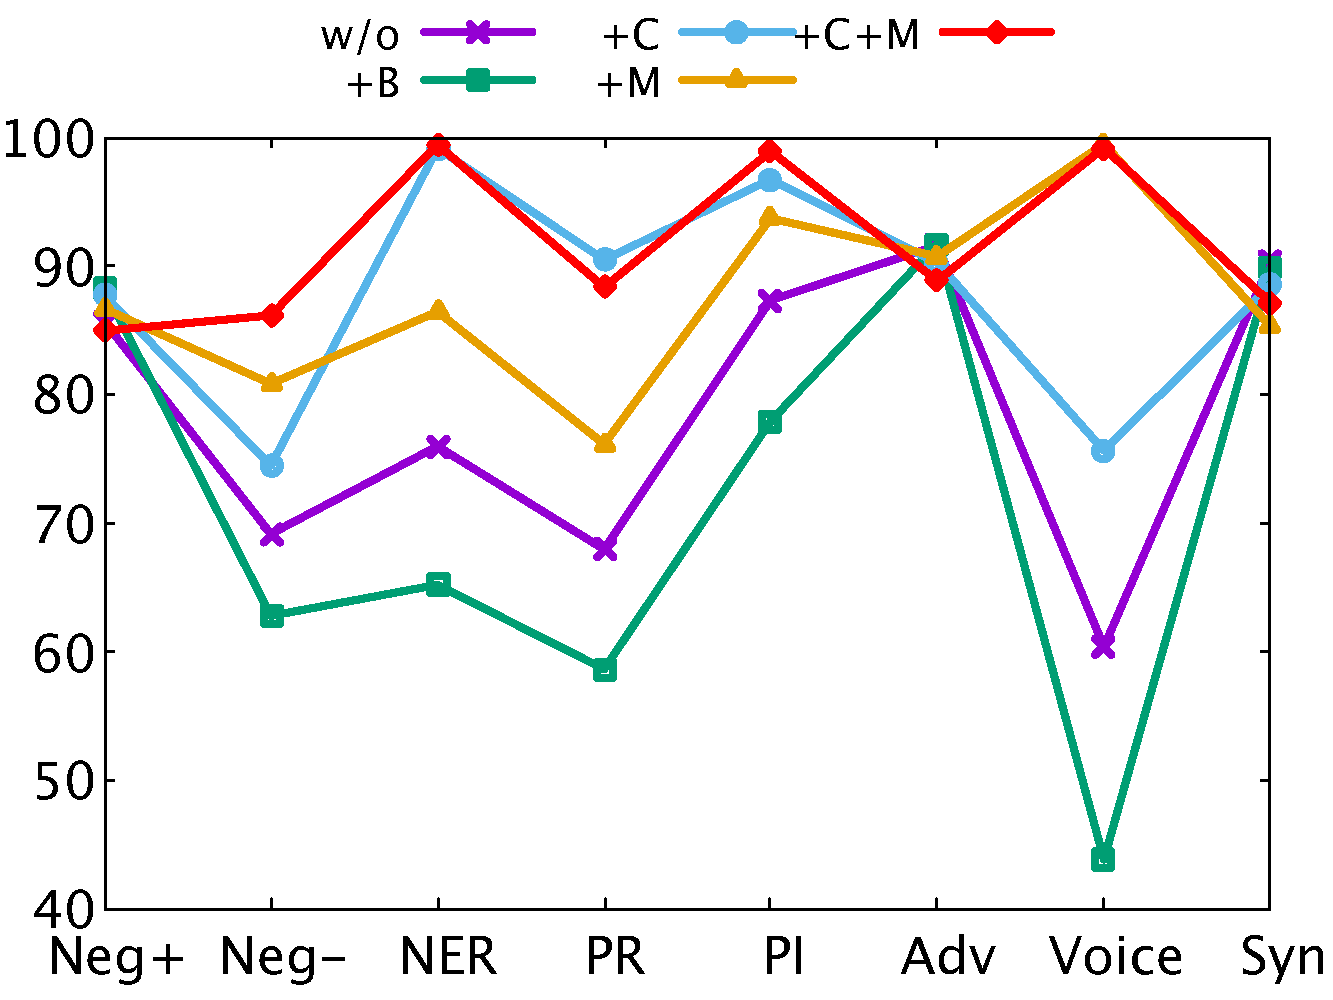
\includegraphics[width=0.6\columnwidth]{data/roc_roberta.pdf}
%   \caption{Detailed stress test with different aspects on ROC dataset. The x-axis indicates different stress test aspects and the y-axis indicates model accuracy in percentage.}
%   \label{fig:detailed}
% \end{figure}


%\begin{figure*}[!th]
%\centering
%\begin{subfigure}[b]{0.28\textwidth}
%\centering
%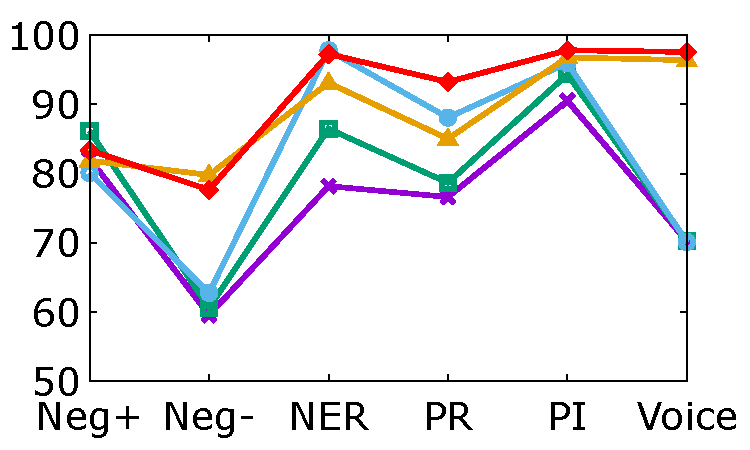
\includegraphics[width=\columnwidth]{data/roc_bert.pdf}
%\caption{BT (ROC)}
%\label{fig:roc_bert}
%\end{subfigure}
%\hfill
%\begin{subfigure}[b]{0.28\textwidth}
%\centering
%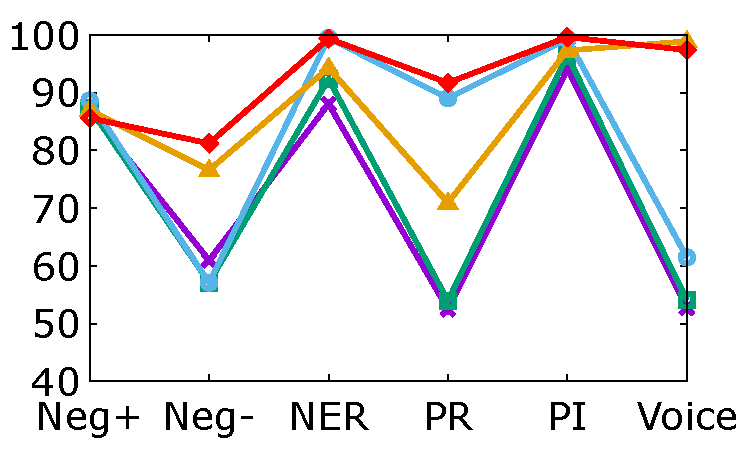
\includegraphics[width=\columnwidth]{data/roc_xlnet.pdf}
%\caption{XL (ROC)}
%\label{fig:roc_xlnet}
%\end{subfigure}
%\hfill
%\begin{subfigure}[b]{0.28\textwidth}
%\centering
%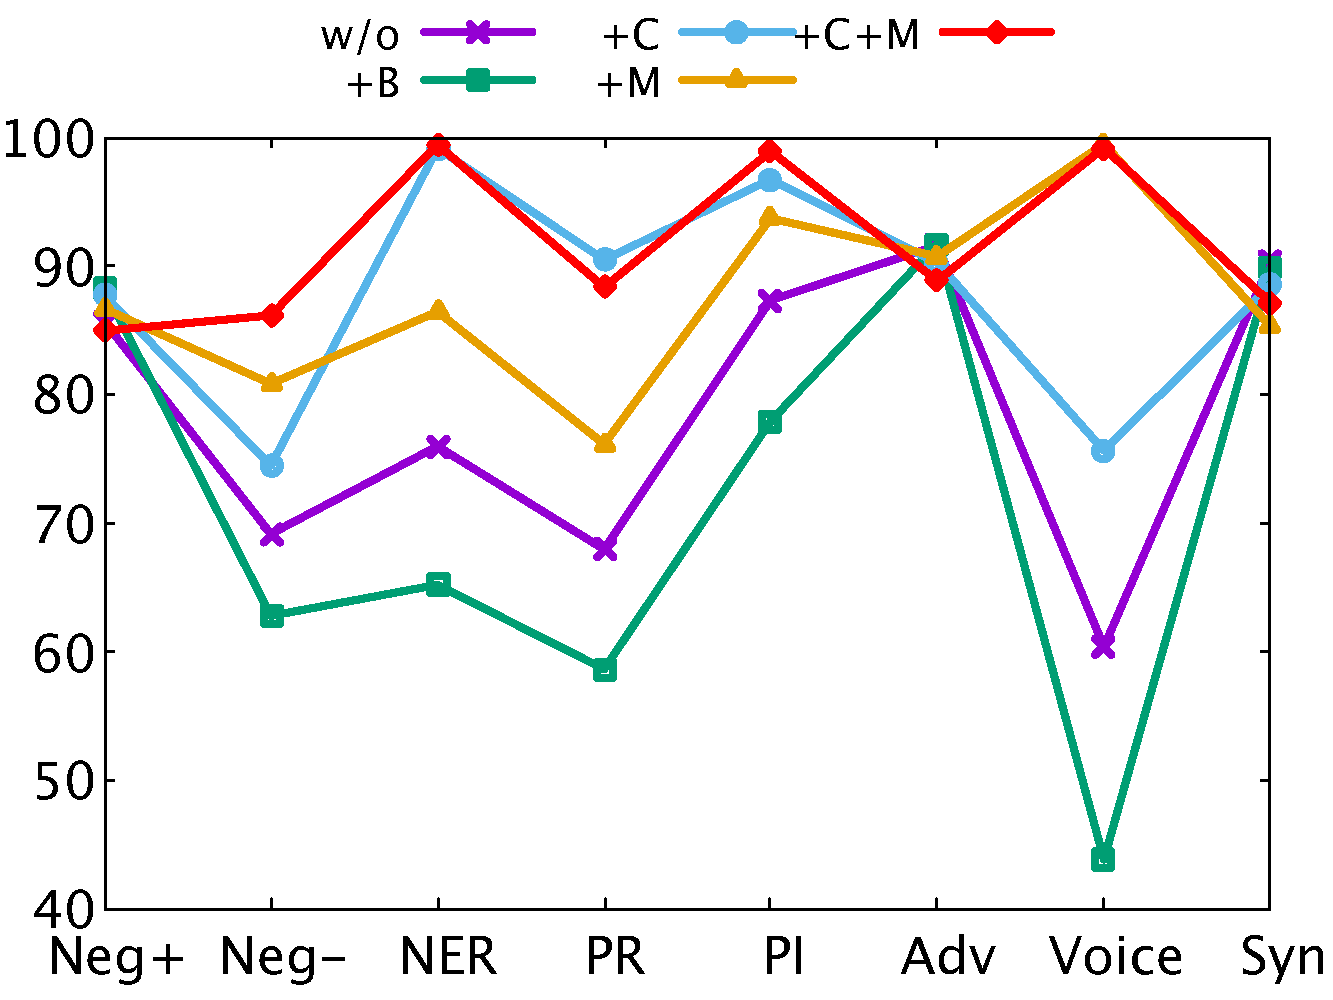
\includegraphics[width=\columnwidth]{data/roc_roberta.pdf}
%\caption{RB (ROC)}
%\label{fig:roc_roberta}
%\end{subfigure}
%\newpage
%\begin{subfigure}[b]{0.28\textwidth}
%\centering
%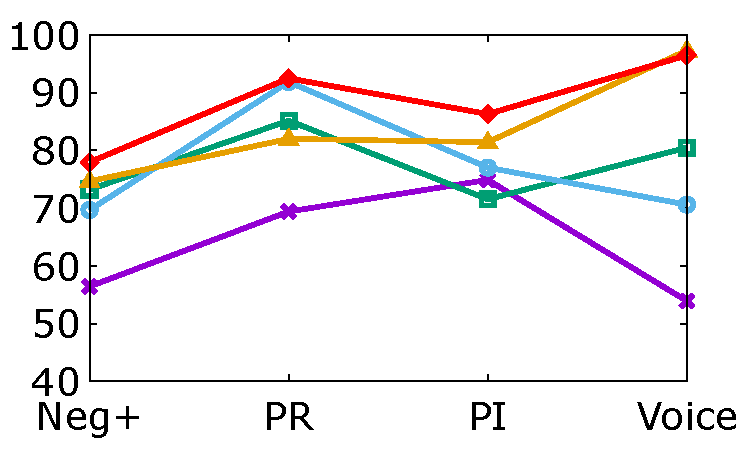
\includegraphics[width=\columnwidth]{data/copa_bert.pdf}
%\caption{BT (COPA)}
%\label{fig:copa_bert}
%\end{subfigure}
%\hfill
%\begin{subfigure}[b]{0.28\textwidth}
%\centering
%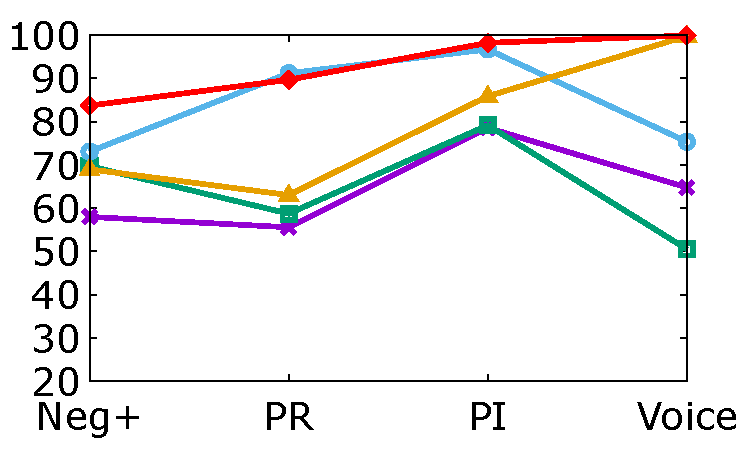
\includegraphics[width=\columnwidth]{data/copa_xlnet.pdf}
%\caption{XL (COPA)}
%\label{fig:copa_xlnet}
%\end{subfigure}
%\hfill
%\begin{subfigure}[b]{0.28\textwidth}
%\centering
%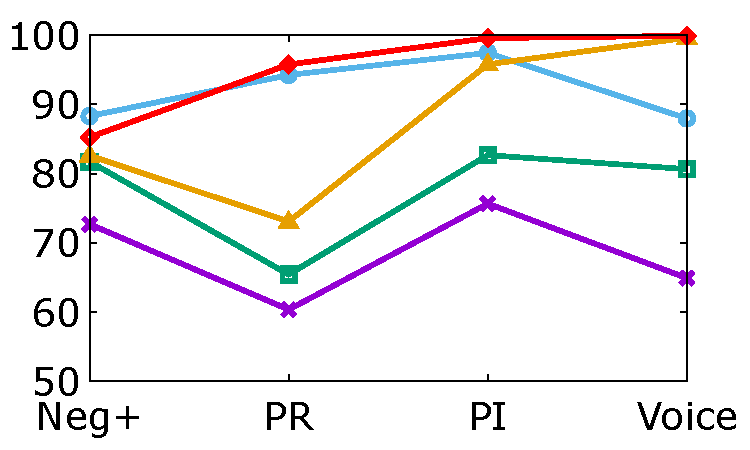
\includegraphics[width=\columnwidth]{data/copa_roberta.pdf}
%\caption{RB (COPA)}
%\label{fig:copa_roberta}
%\end{subfigure}
%\newpage
%\begin{subfigure}[b]{0.28\textwidth}
%\centering
%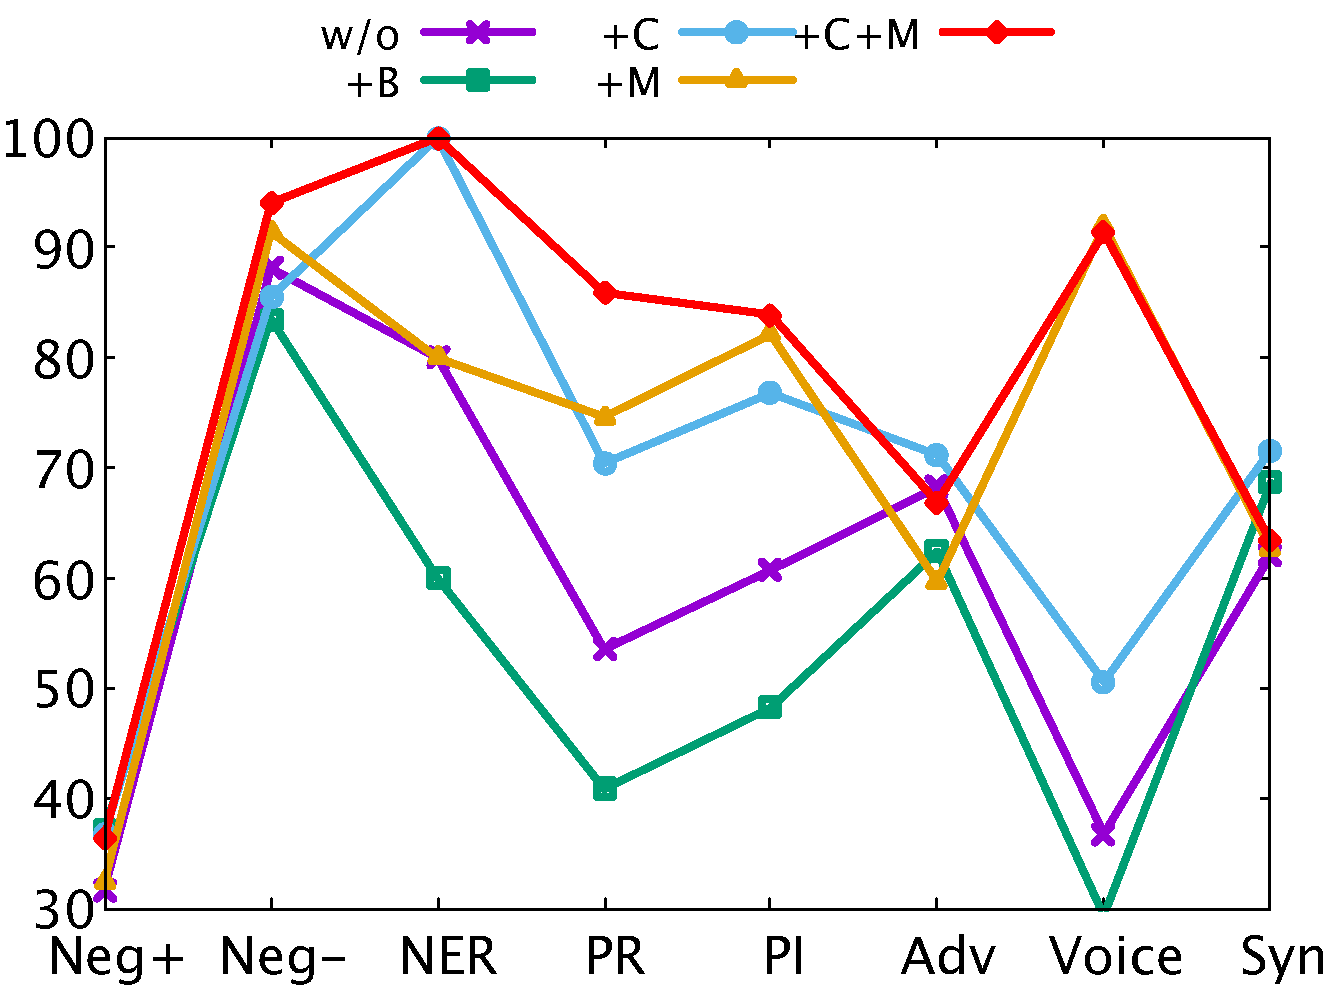
\includegraphics[width=\columnwidth]{data/arct_bert.pdf}
%\caption{BT (ARCT)}
%\label{fig:arct_bert}
%\end{subfigure}
%\hfill
%\begin{subfigure}[b]{0.28\textwidth}
%\centering
%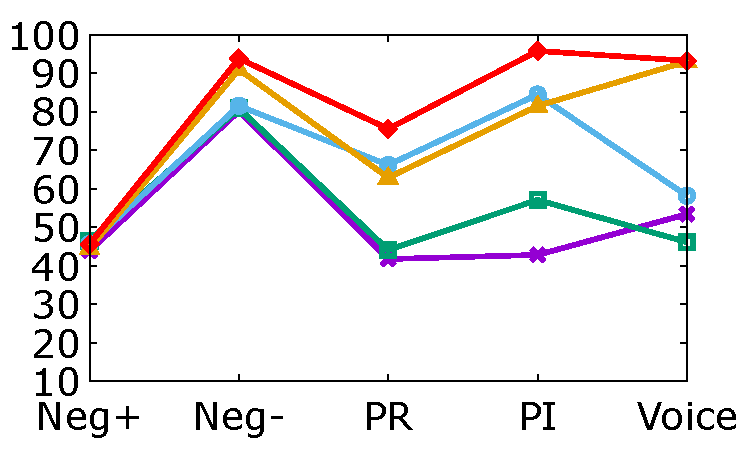
\includegraphics[width=\columnwidth]{data/arct_xlnet.pdf}
%\caption{XL (ARCT)}
%\label{fig:arct_xlnet}
%\end{subfigure}
%\hfill
%\begin{subfigure}[b]{0.28\textwidth}
%\centering
%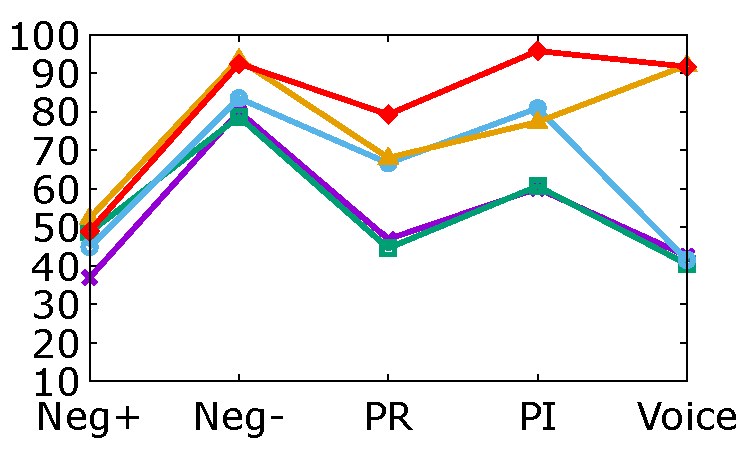
\includegraphics[width=\columnwidth]{data/arct_roberta.pdf}
%\caption{RB (ARCT)}
%\label{fig:arct_roberta}
%\end{subfigure}
%\newpage
%\begin{subfigure}[b]{0.28\textwidth}
%\centering
%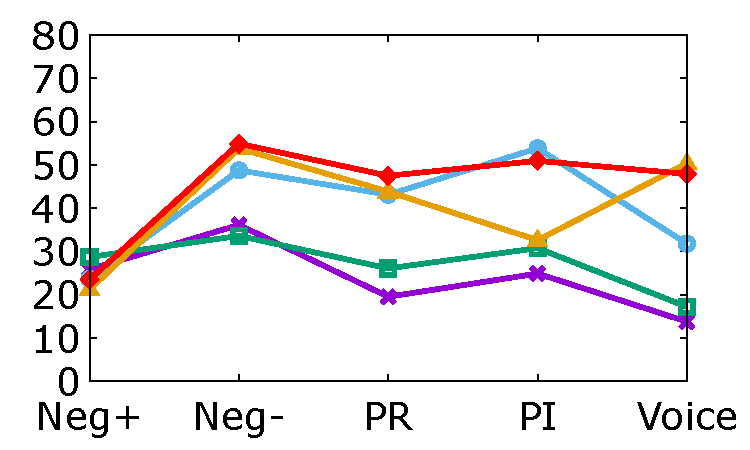
\includegraphics[width=\columnwidth]{data/reclor_bert.pdf}
%\caption{BT (RECLOR)}
%\label{fig:reclor_bert}
%\end{subfigure}
%\hfill
%\begin{subfigure}[b]{0.28\textwidth}
%\centering
%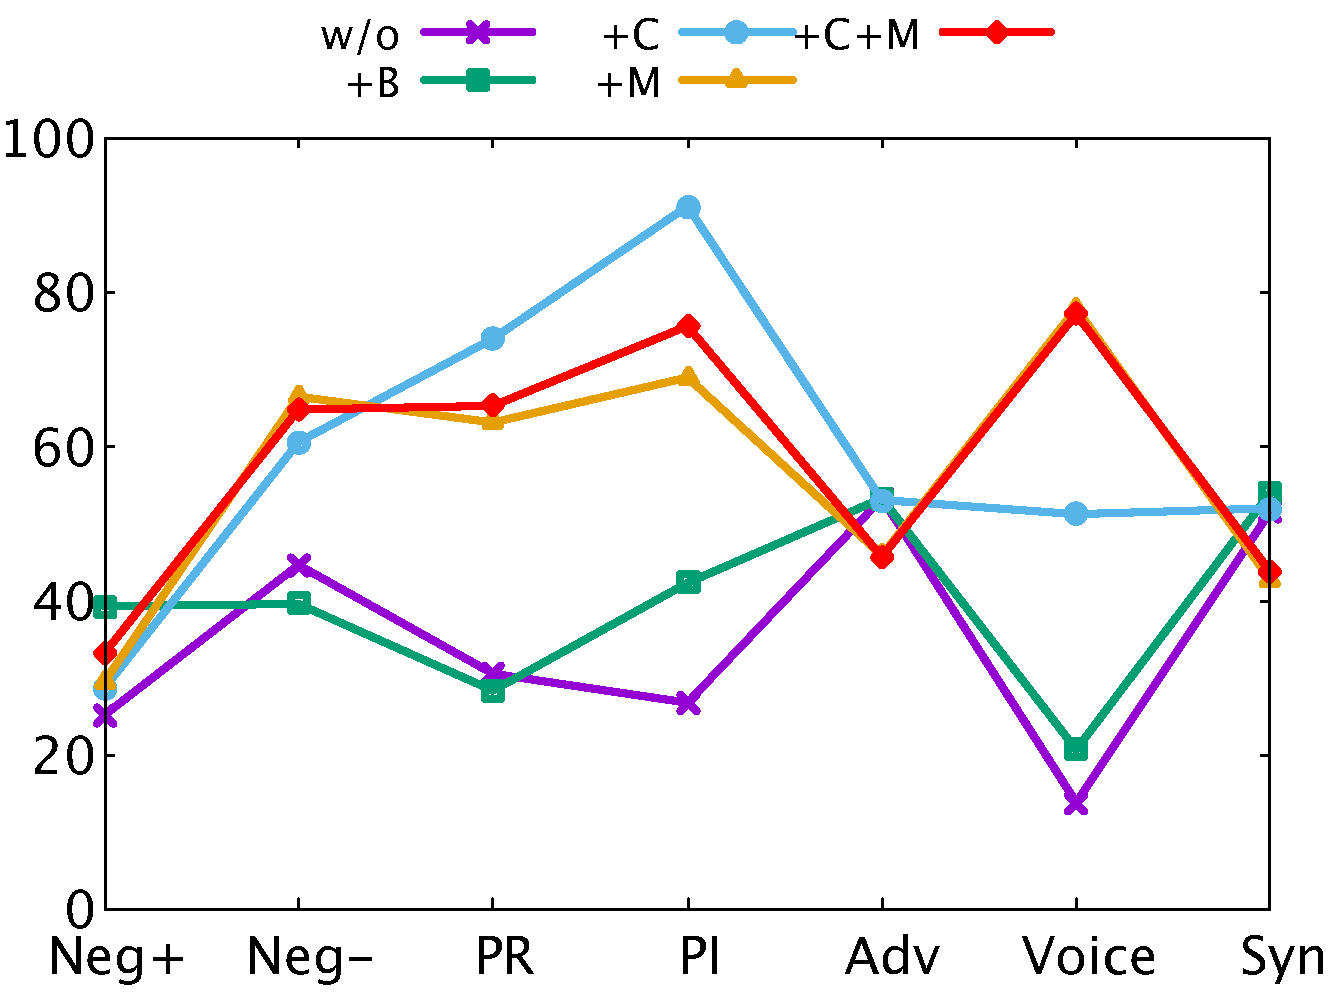
\includegraphics[width=\columnwidth]{data/reclor_xlnet.pdf}
%\caption{XL (RECLOR))}
%\label{fig:reclor_xlnet}
%\end{subfigure}
%\hfill
%\begin{subfigure}[b]{0.28\textwidth}
%\centering
%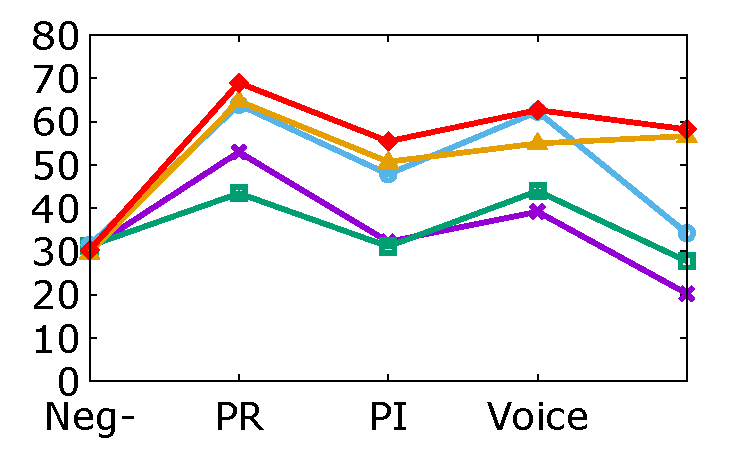
\includegraphics[width=\columnwidth]{data/reclor_roberta.pdf}
%\caption{RB (RECLOR)}
%\label{fig:arct_roberta}
%\end{subfigure}
%\newpage
%\begin{subfigure}[b]{1.0\textwidth}
%\centering
%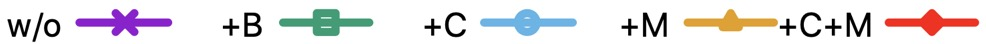
\includegraphics[width=0.4\columnwidth]{data/label.jpg}
%\label{fig:label}
%\end{subfigure}
%\caption{Fine-grained stress test with different aspects on 4 different tasks. 
%The x-axis in the figures indicates different stress test aspects and the y-axis indicates model accuracy in percentage.}
%%\KZ{Caption is wrong! most graphs are fine. 
%%But ReCLOR (RB) is a bit strange. 
%%Why is BT line exactly the same as the BT+C? And why is BT+B so bad?}}
%\label{fig:detail}
%\end{figure*}
%%
%
\begin{figure*}[!th]
\centering
\begin{subfigure}[b]{0.24\textwidth}
\centering
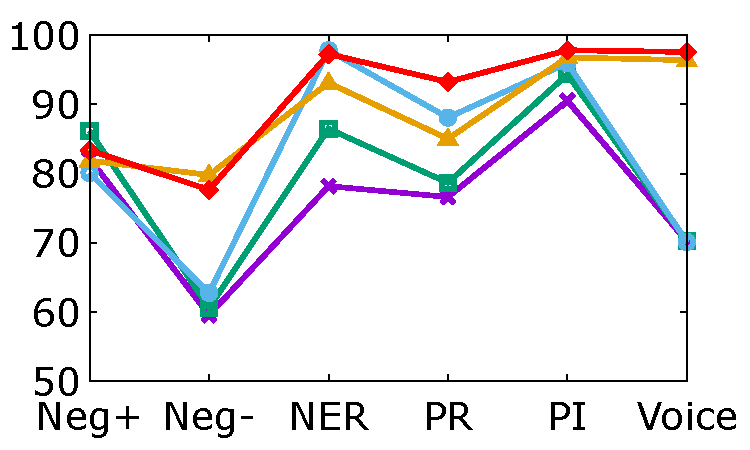
\includegraphics[width=\columnwidth]{data/roc_bert.pdf}
\caption{BT (ROC)}
\label{fig:roc_bert}
\end{subfigure}
\hfill
\begin{subfigure}[b]{0.24\textwidth}
\centering
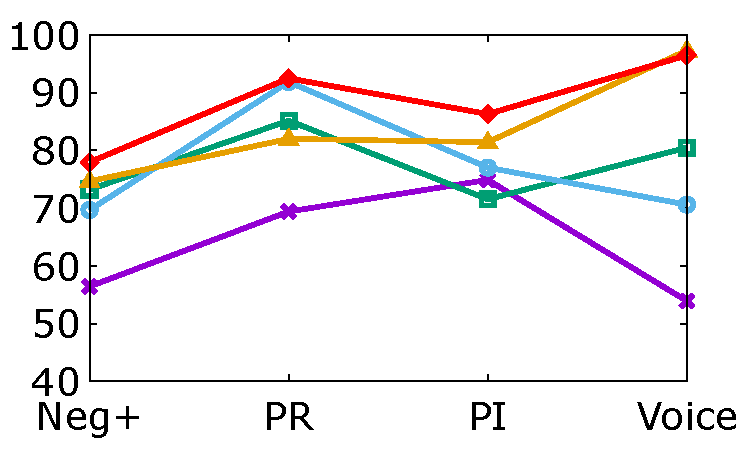
\includegraphics[width=\columnwidth]{data/copa_bert.pdf}
\caption{BT (COPA)}
\label{fig:copa_bert}
\end{subfigure}
\hfill
\begin{subfigure}[b]{0.24\textwidth}
\centering
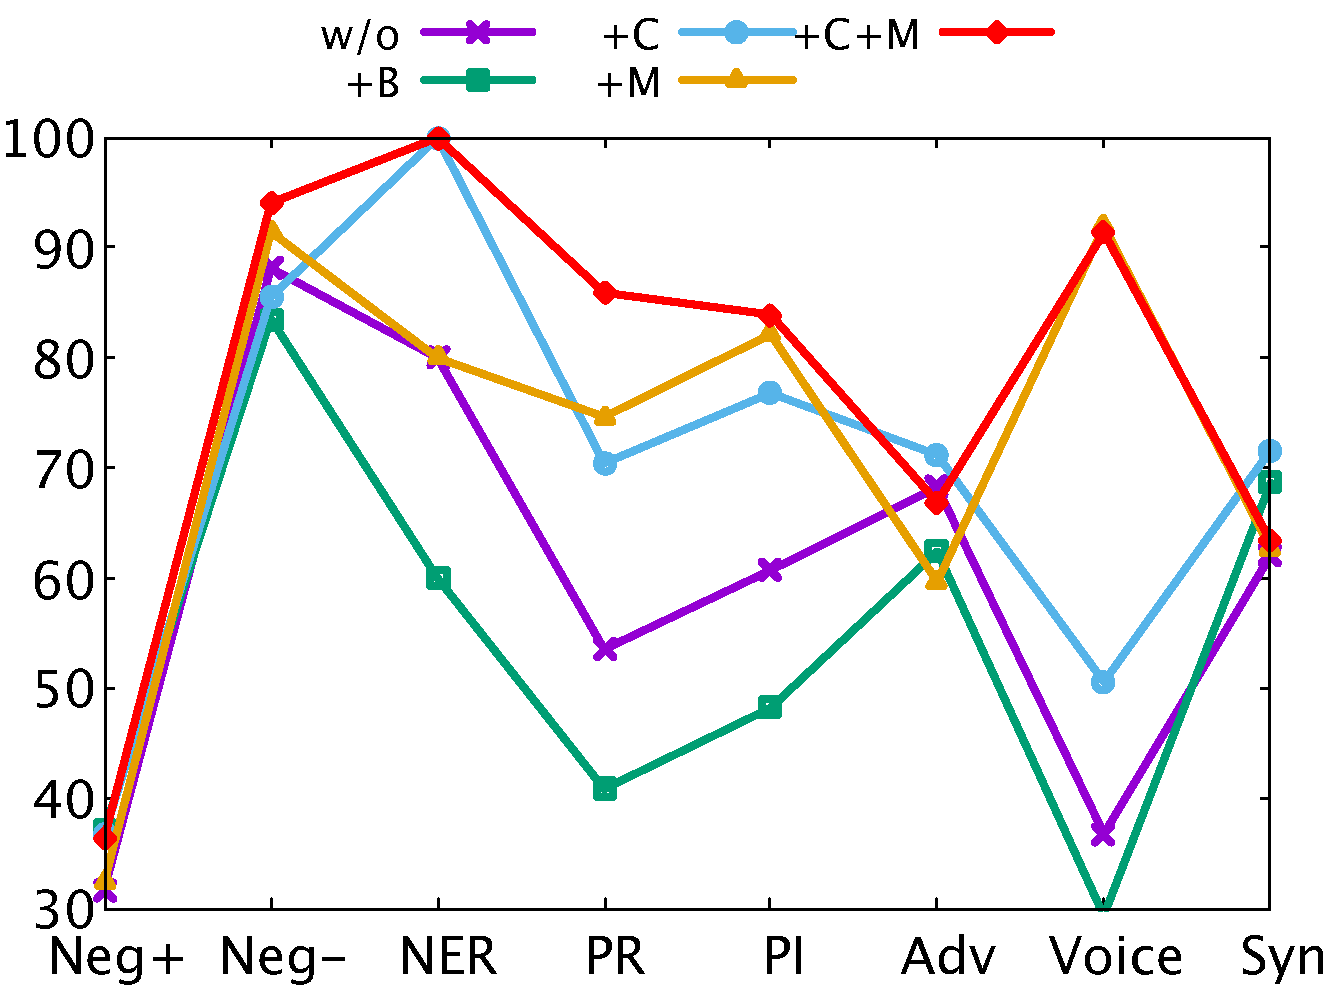
\includegraphics[width=\columnwidth]{data/arct_bert.pdf}
\caption{BT (ARCT)}
\label{fig:arct_bert}
\end{subfigure}
\hfill
\begin{subfigure}[b]{0.24\textwidth}
\centering
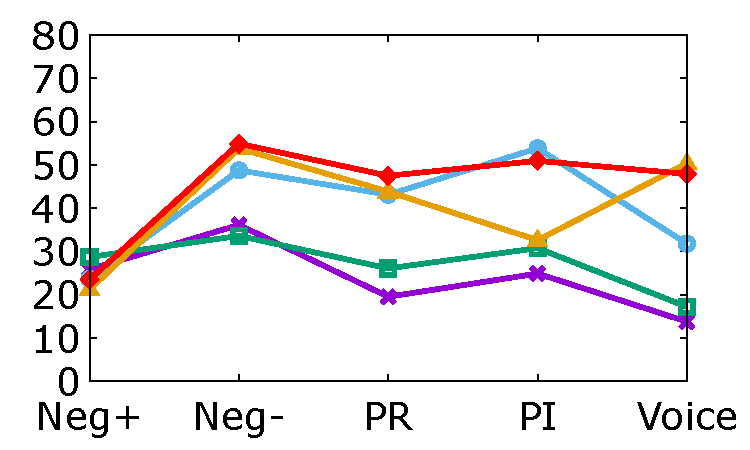
\includegraphics[width=\columnwidth]{data/reclor_bert.pdf}
\caption{BT (RECLOR)}
\label{fig:reclor_bert}
\end{subfigure}
\newpage
\begin{subfigure}[b]{0.24\textwidth}
\centering
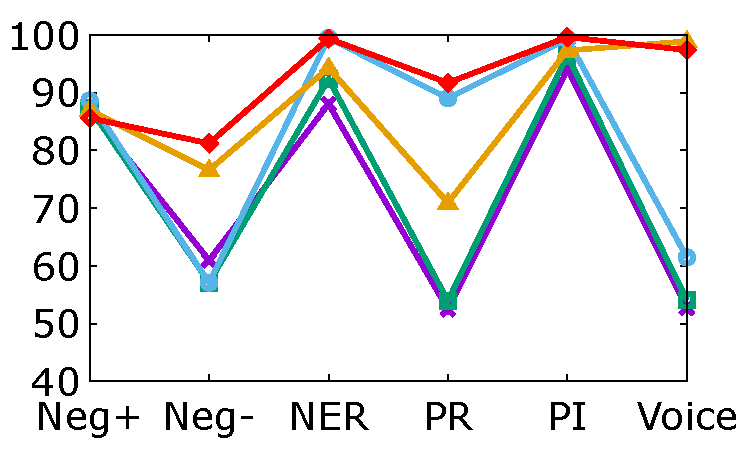
\includegraphics[width=\columnwidth]{data/roc_xlnet.pdf}
\caption{XL (ROC)}
\label{fig:roc_xlnet}
\end{subfigure}
\hfill
\begin{subfigure}[b]{0.24\textwidth}
\centering
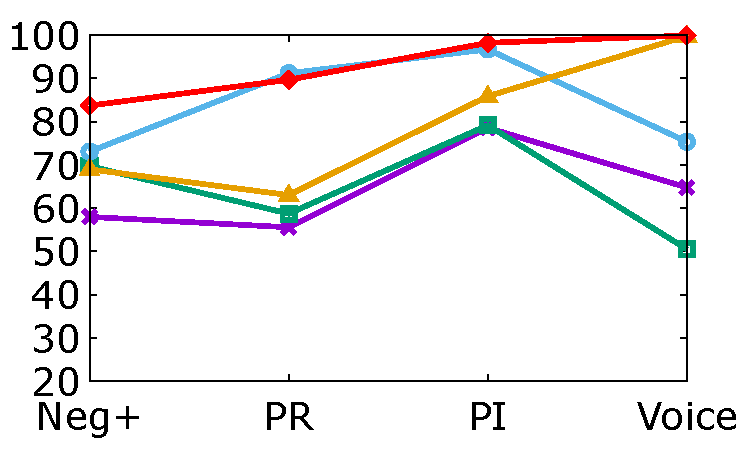
\includegraphics[width=\columnwidth]{data/copa_xlnet.pdf}
\caption{XL (COPA)}
\label{fig:copa_xlnet}
\end{subfigure}
\hfill
\begin{subfigure}[b]{0.24\textwidth}
\centering
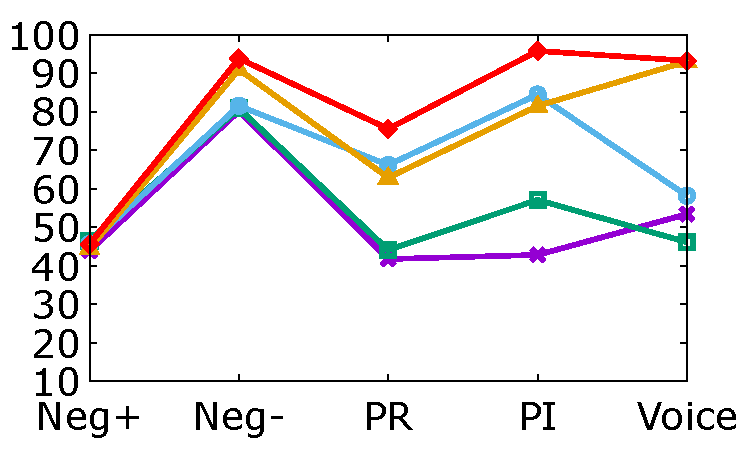
\includegraphics[width=\columnwidth]{data/arct_xlnet.pdf}
\caption{XL (ARCT)}
\label{fig:arct_xlnet}
\end{subfigure}
\hfill
\begin{subfigure}[b]{0.24\textwidth}
\centering
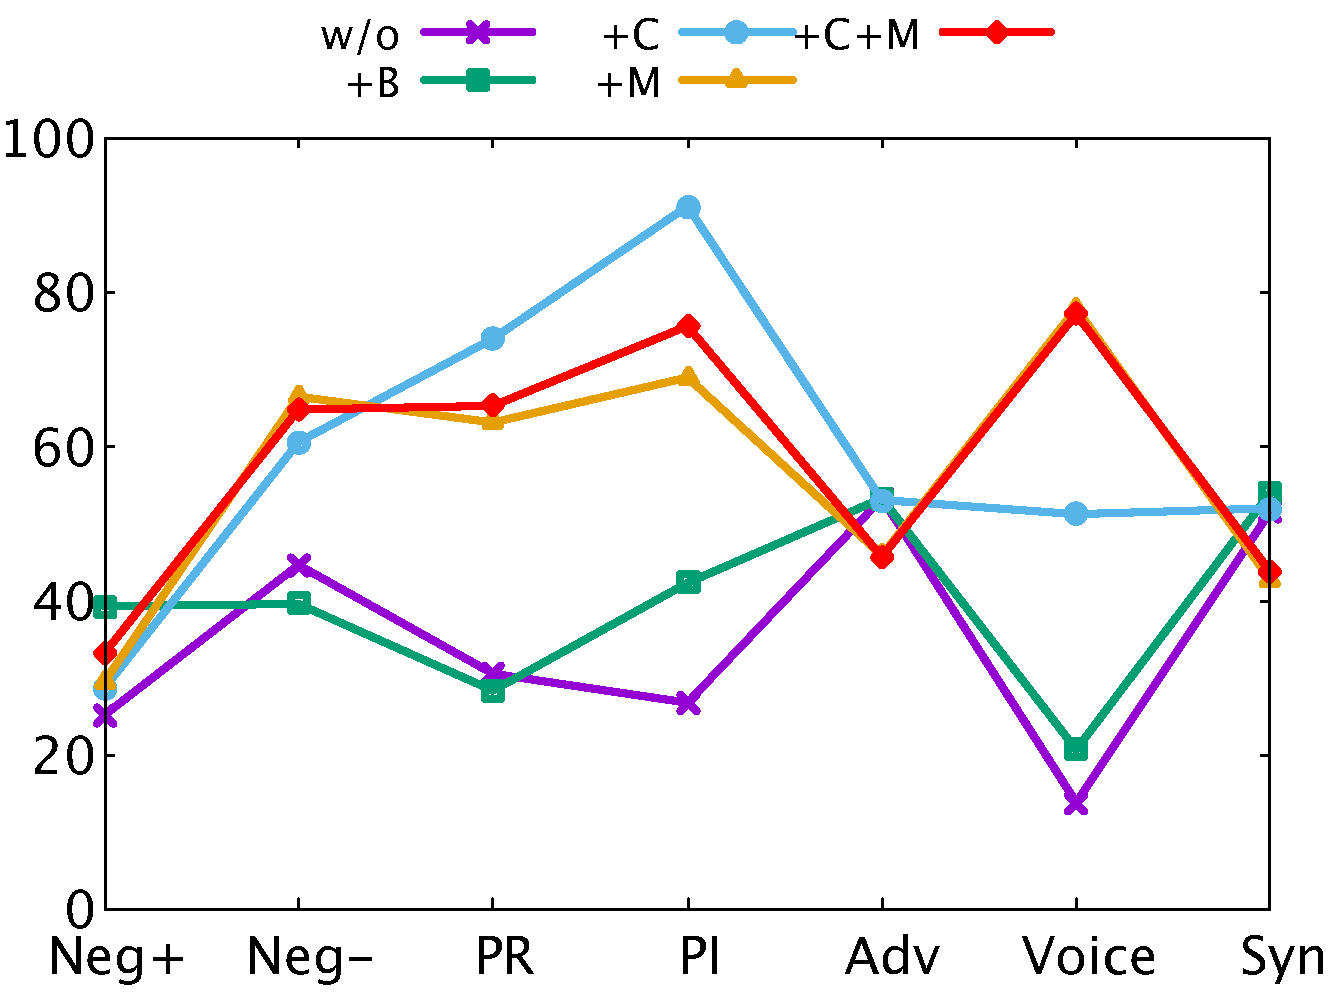
\includegraphics[width=\columnwidth]{data/reclor_xlnet.pdf}
\caption{XL (RECLOR))}
\label{fig:reclor_xlnet}
\end{subfigure}
\newpage
\begin{subfigure}[b]{0.24\textwidth}
\centering
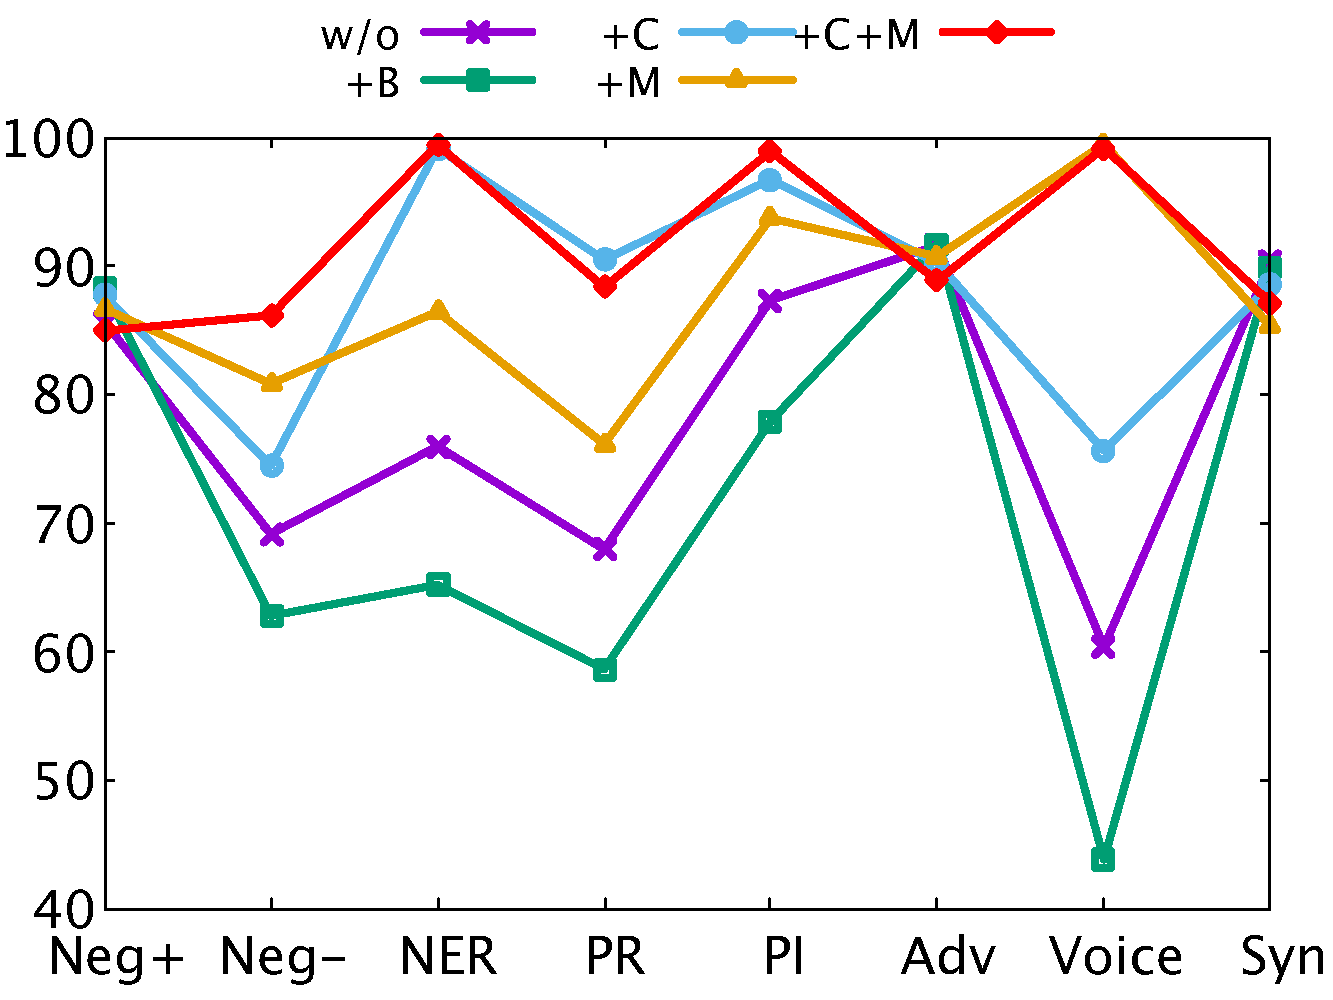
\includegraphics[width=\columnwidth]{data/roc_roberta.pdf}
\caption{RB (ROC)}
\label{fig:roc_roberta}
\end{subfigure}
\hfill
\begin{subfigure}[b]{0.24\textwidth}
\centering
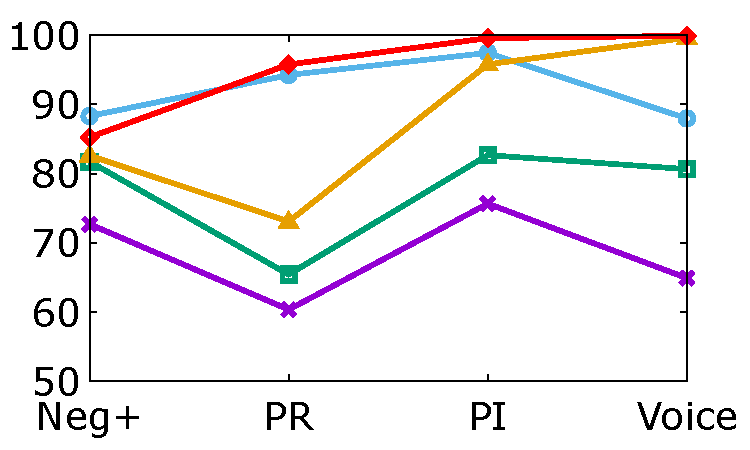
\includegraphics[width=\columnwidth]{data/copa_roberta.pdf}
\caption{RB (COPA)}
\label{fig:copa_roberta}
\end{subfigure}
\hfill
\begin{subfigure}[b]{0.24\textwidth}
\centering
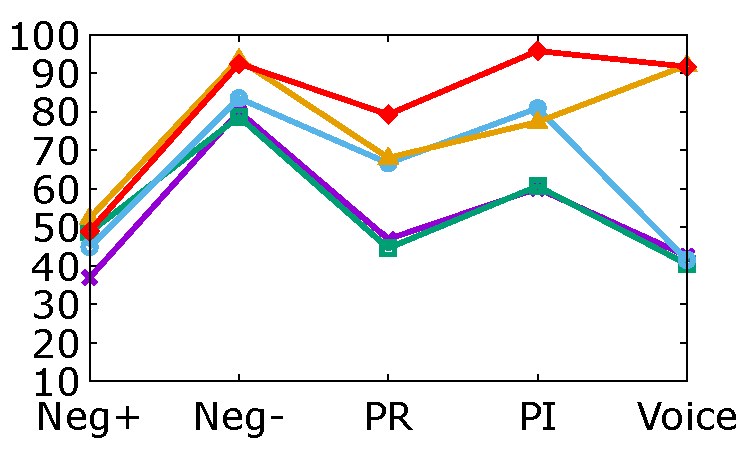
\includegraphics[width=\columnwidth]{data/arct_roberta.pdf}
\caption{RB (ARCT)}
\label{fig:arct_roberta}
\end{subfigure}
\hfill
\begin{subfigure}[b]{0.24\textwidth}
\centering
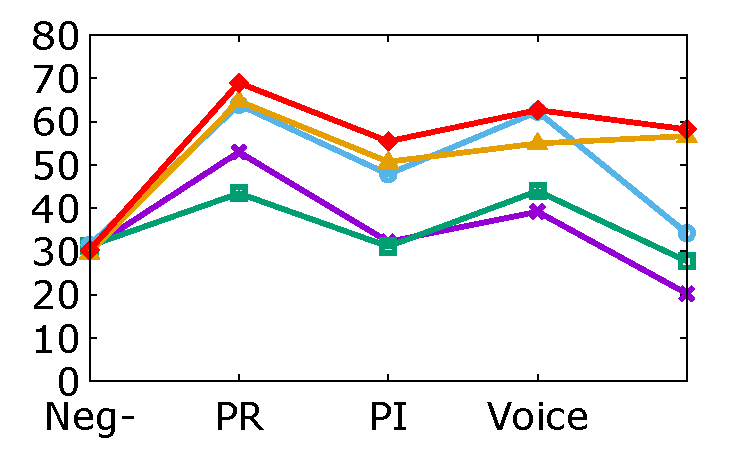
\includegraphics[width=\columnwidth]{data/reclor_roberta.pdf}
\caption{RB (RECLOR)}
\label{fig:arct_roberta}
\end{subfigure}
\newpage
\begin{subfigure}[b]{1.0\textwidth}
\centering
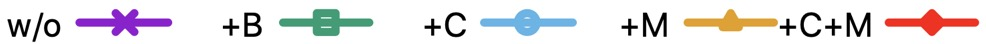
\includegraphics[width=0.4\columnwidth]{data/label.jpg}
\label{fig:label}
\end{subfigure}
\caption{Fine-grained stress test with different aspects on 4 different tasks. 
The x-axis in the figures indicates different stress test aspects and the y-axis indicates model accuracy in percentage.}
%\KZ{Caption is wrong! most graphs are fine. 
%But ReCLOR (RB) is a bit strange. 
%Why is BT line exactly the same as the BT+C? And why is BT+B so bad?}}
\label{fig:detail}
\end{figure*}
%
\subsubsection{Fine-grained results}
\label{sec:fine-grained}
We proceed to break down the results in \tabref{tab:stressresults} into accuracies on stress tests
created by different operators. 
%We show the detailed results in~\figref{fig:detail} 
%Concretely, six different aspects of stress test data are 
%utilized for testing.
COPA and RECLOR datasets do not show all six operators
because some of the operators generate too little data
for them, as shown in \tabref{tab:cases}. 
%The x-axis in the figures indicates different stress test aspects 
%and the y-axis indicates model accuracy in percentage.
%We apply the proposed two operators \textit{crossover} and \textit{mutation} to BERT, XLNet and RoBERTa 
%models and compare it with back-translation.
%and test on various stress test cases with different aspects. 
The corresponding results are presented in~\figref{fig:detail}. 
We observe that the vanilla model in purple and back-translation in green show
worse results across different aspects than other lines. 
The models trained with data augmented by \textit{crossover} and \textit{mutation} 
(the red lines) are generally more robust than others.
%\KZ{It is consistent with our overall results in~\tabref{tab:results}.} 
Please refer to Appendix A. 
%\footnote{There are some dashes in the table because the } 
for complete results. 
%\KZ{You need to explain why there are some dashes in the table in appendix.}

%We also observe that the 
%accuracy performance points for ``Syn'' and ``Adv'' are concentrated 
%but scattered on other operator aspects. 
Since every type of stress tests 
%(except ``Syn'' and ``Adv) 
can evaluate if a model is robust, particularly if it considers the 
premise by giving it two very similar choices, 
the above results on the stress tests of all types show that our two methods do 
%improves the model robustness, and may even encourage the models to look toward the
reduce short-circuits, and may even encourage the models to look toward the
premises.
We will provide additional pieces of evidence to confirm this in the next two subsections.

%\KZ{The weakness can be on the same table as the improvements
%to save space.}
%\KZ{Check the following analysis to make sure it's consistent with the tables.}

%Compared with 
%base models without data augmentation, we find that 
%all four data augmentation methods moderately improve
%the models when tested on the original test set. 
%In ROC, accuracy of BERT and RoBERTa trained with crossover augmented data 
%exceeds base models and ranks top. Crossover method also works on COPA. 
%Even though back-translation obtains higher score mostly on ARCT and RECLOR,
%crossover, mutation and crossover+mutation barely fall below the base model. 
%
%Augmentation fares much better in the ``Stress'' columns, though
%different methods show varying degree of success.
%Compared with the model without data augmentation, 
%the performance of models with crossover 
%has always been greatly improved (i.e., by 21.44\% for BERT on COPA).
%It indicates that reducing the short circuits 
%is a good way to improve the robustness of a model.
%The performance of new models with crossover has 
%great improvement for all models on different dataset 
%compared with the model without data augmentation, like 21.44% for BERT on COPA. 
%Mutation alone can also help with robustness on stress test better than crossover.
%This result suggests that mutation is a good method 
%for enhancing the robustness of models. 
%Though, mutation may be not a 
%good method to decrease the short circuits (\secref{sec:fix-sc}). 
%Overall, crossover+mutation 
%can mostly get the best performance on the stress test except for 
%training on RECLOR with RoBERTa. 
%to This result indicates that this kind of data can prevent models from being confused 
%by simple perturbations thus improving the robustness of models. 
%Besides, we can also find that back-translation doesn't improve the models' robustness much.
%Crossover alone can also help with robustness on stress test but 
%no better than mutation and crossover+mutation.  

%some of Table 5's AW scores being 
%some of Table 5's AW scores being 
%lower than AW for model w/o augmentation (e.g., 45.13 in (b)), 
%then the reason is AW is only a proxy test
%that catches majority of short circuit cases in our opinion, 
%but it's not perfect, as we pointed out in A2 of R1. 
%If you are referring to some accuracies in the Original columns 
%being lower than models w/o augmentation in Table 5 (e.g., 72.6 in (b)), 
%the reason is some models w/o augmentation might have 
%"cheated" to get high accuracy. Augmenting (C or M) corrects the
%biases in these models and may reduce the accuracy on the original test set.
%Nevertheless, all models after augmentation do better on the stress tests.

%have least short circuits based on BERT and XLNet. 
%Crossover+mutation based on RoBERTa takes less short circuits than others. 
%In the CO and AW columns, the result are consistent on ROC. 

%\subsection{White-box Attention Weights~(AW)}
%\KZ{Here we first talk about human testing by visualizastion,
%then talk about how to automatic it thru code.}

%show human annotation results of bert, roberta, xlnet.
%For exploiting whether attention-based models are suffered from short circuits, 
%we propose to 
%use the AW method which we have described in~\secref{}.
%It is noted that t\_1 is greater than t\_2. 
%Here t\_1 and t\_2 are tuned to 0.14 and 0.13 separately.

\subsection{Choice-only Test}
\label{sec:choice-only}

%In this section, we use choice-only test for different models on four tasks. 
%We have shown the effectiveness of \textit{crossover} and \textit{mutation} on in robustness test. 
The end-to-end test has shown the success of our data augmentation 
methods. To further explore the reason behind the performance gain, 
we also use choice-only test here.

%somewhat confirm the reason for model improvement with data augmentation 
%strategies. Moreover, this test is used to further explore 
%whether our strategies can encourage models pay more attention to premise.
In choice-only test, we only feed choices into a model without a premise which is replaced 
by an empty string. This way, 
models cannot utilize the relationship between premise and choices. 
%what we can know whether a model can 
%solve cases easily without awaring premise by test accuracy. 
Normally, we would expect the model to make arbitrary choices.
However, if a model can easily ``guess'' the ``right'' choice which 
normally requires the relationship between premise and choices,  
one possibility is that this model cheats on evaluation procedure and 
may be fragile. Thus, the higher score may indicate more use of short-circuits.

In~\figref{fig:choice-only}, we observe that in choice-only tests,
the accuracy of models augmented with \textit{crossover} and \textit{mutation} 
(red line) drops the most. 
Sometimes the performances are similar to random selection, e.g., 
RB+C+M on ARCT (56.38\%), which indicates that models 
are no longer cheating. 
In other words, models augmented by crossover and mutation 
are more likely to consider the premises. 
The results on the choice-only tests provide another perspective for us
to re-assure that models augmented with crossover and mutation can reduce
short circuits and thus model fragility.

%\KZ{Rephrase: 
%However, another possibility reason for lower choice-only test accuracy 
%that is also not ruled out is that 
%even if the model can tell the result with only choices, 
%it still chooses to look at the premise context. 
%Although high scores do not necessarily imply models 
%are not looking forward, low scores necessarily mean that models cannot 
%conclude that solely relying on choices.} 

%\begin{table}[th]
%\centering
%\scriptsize
%\begin{tabular}{c|rrrr}
%\toprule
%\textbf{Model} & \textbf{ROC} & \textbf{COPA} & \textbf{ARCT} & \textbf{RECLOR} \\ \midrule
%%BT  &98.76 &89.68&\textbf{99.65}&82.46    \\ \hline
%%BT+B  &99.26 &96.79   &99.34  &86.01  \\ \hline
%%BT+C  &\textbf{99.69} &\textbf{98.35}&98.37   &80 \\ \hline
%%BT+M  &99.26 & 95.17 &98.67 &82.48    \\ \hline
%%BT+C+M  &98.82 &96.96 &98.00 &\textbf{96.79}  \\ \midrule
%%XL  &28.08 &93.16 & 85.67 & 79.64 \\ \hline
%%XL+B  &19.27  &91.46 &95.73 & 81.40   \\ \hline
%%XL+C  &\textbf{64.58} &45.13  &55.59  &\textbf{87.87} \\ \hline
%%XL+M  &62.77  &96.85 & \textbf{95.74}& 72.76  \\ \hline
%%XL+C+M  &60.25 & \textbf{98.51}&86.26 &   48.71\\ \midrule
%%RB  &77.41 & 80.89 & 99.14& 85.88 \\ \hline
%%RB+B  &   58.15 &\textbf{96.36}   & 97.78& 15.69  \\ \hline
%%RB+C  &   82.71& 89.62&79.19& 89.68\\ \hline
%%RB+M  &71.73& 62.26& \textbf{100.00}&\textbf{100.00}  \\ \hline
%%RB+C+M  &\textbf{93.31} &61.89    &71.47 & 89.26\\ 
%%
%BT (w/o)&54.62&51.4&61.94&42.8 \\ \hline
%BT+B&58.26&50.8&64.41&39.2  \\ \hline
%BT+C&51.2&48.2&55.63&30.8  \\ \hline
%BT+M&51.79&48.8&55.18&38   \\ \hline
%BT+C+M&43.56&49.4&52.03&33.8  \\ \midrule
%XL (w/o)&71.14&57&65.99&42.2 \\ \hline
%XL+B&73.17&60&66.89&41.4  \\ \hline
%XL+C&65.63&55&55.86&34.2  \\ \hline
%XL+M&71.94&57.8&66.22&42  \\ \hline
%XL+C+M&66.22&58.4&62.84&35  \\ \midrule
%RB (w/o)&73.97&59.4&67.79&30.2 \\ \hline
%RB+B&74.77&61.4&69.37&42.2  \\ \hline
%RB+C&73.06&58.4&68.47&34.6  \\ \hline
%RB+M&70.34&56&61.49&40      \\ \hline
%RB+C+M&71.3&54.8&67.79&32.2  \\ 
%\bottomrule
%\end{tabular}
%\caption{Choice-only test for transformer-based models on 4 datasets. All numbers are percentages (\%)}
%%\KZ{I assume this is the ending-only test? But isn't scriptsizeer the better
%%for ending-only tests?}}
%\label{tab:only-test}
%\end{table}
%
\begin{figure}[th]
    \centering
    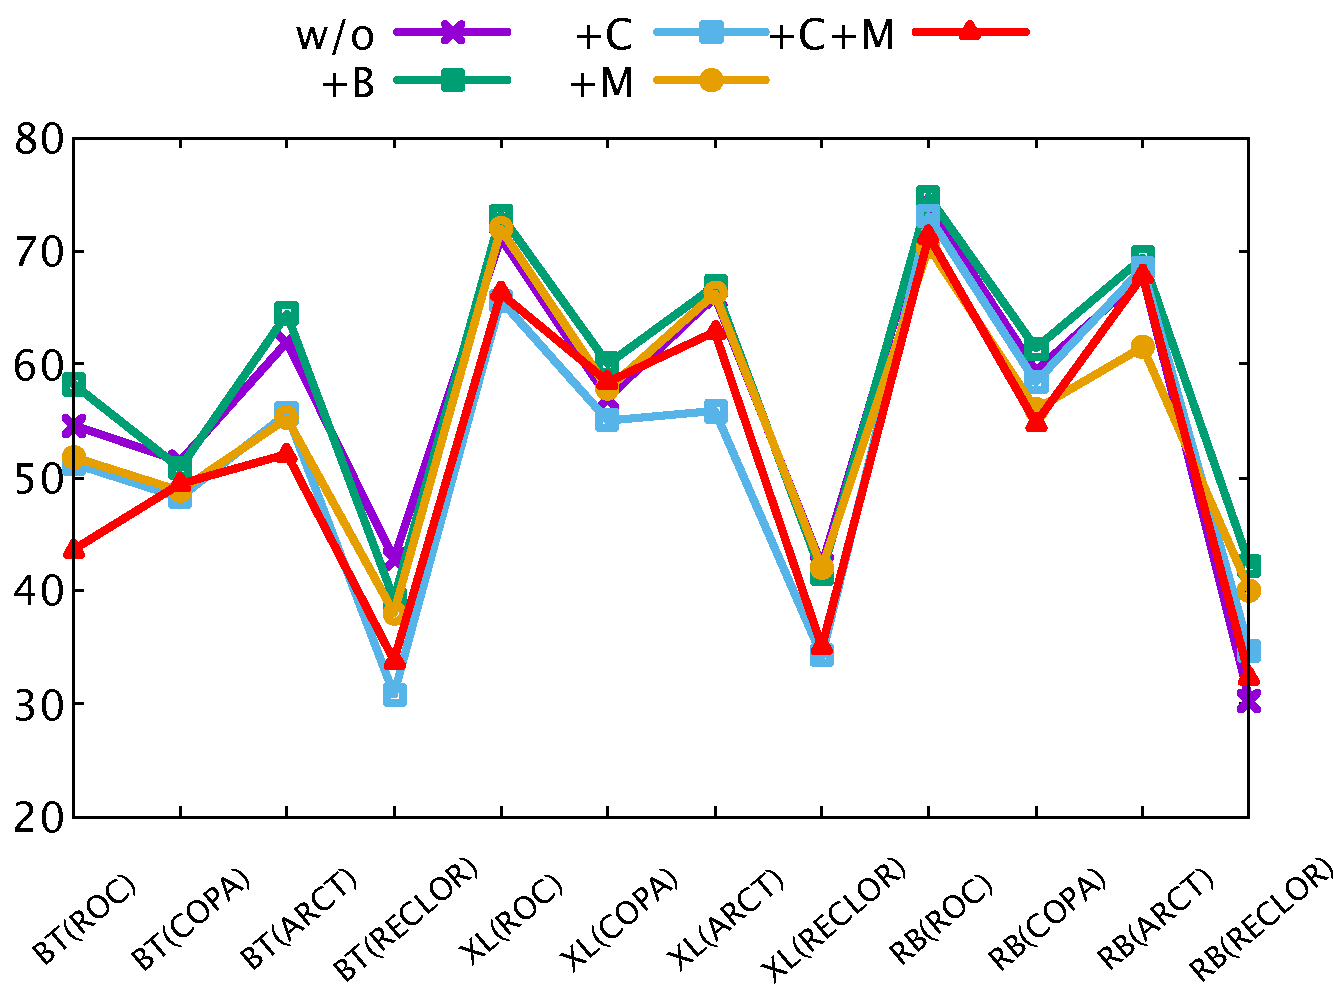
\includegraphics[width=0.7\columnwidth]{data/choice-only.pdf}
    \caption{Choice-only test: Accuracies of different data augmentation methods with 3 models on 4 tasks. 
    The detailed numbers are in Appendix B.}
    \label{fig:choice-only}
\end{figure}

However, one may argue that even if a model can 
choose or ``guess'' correctly given only the choices but no premise, 
it may still have the ability to look at the premise if it's given one,
like in the end-to-end test.
Therefore, next we conduct an additional case study to show that short-circuit
does take place and our augmentation methods alleviate it.

\subsection{Case Study}
\label{sec:case}

%\begin{figure}[th!]
%\centering
%\begin{subfigure}[b]{0.21\textwidth}
%\centering
%
%\framebox{\includegraphics[width=\columnwidth]{figure/case_original.eps}}
%\caption{RB(w/o)}
%\label{fig:case_original}
%\end{subfigure}
%\hfill
%\begin{subfigure}[b]{0.21\textwidth}
%\centering
%\framebox{\includegraphics[width=\columnwidth]{figure/case_b.eps}}
%\caption{RB+B}
%\label{fig:case_b}
%\end{subfigure}
%\hfill
%\newpage
%\begin{subfigure}[b]{0.21\textwidth}
%\centering
%\framebox{\includegraphics[width=\columnwidth]{figure/case_c.eps}}
%\caption{RB+C}
%\label{fig:case_c}
%\end{subfigure}
%\hfill
%\begin{subfigure}[b]{0.21\textwidth}
%\centering
%\framebox{\includegraphics[width=\columnwidth]{figure/case_cm.eps}}
%\caption{RB+C+M}
%\label{fig:case_cm}
%\end{subfigure}
%\caption{Attention map on a COPA example for models.}
%%\KZ{Caption is wrong! most graphs are fine. 
%%But ReCLOR (RB) is a bit strange. 
%%Why is BT line exactly the same as the BT+C? And why is BT+B so bad?}}
%\label{fig:case}
%\end{figure}
%

%In \figref{fig:case}, 
%%illustration. There is no positive attention value in front of the 
%%fourth sentence, so we intercept it from where it is worth. 
%RoBERTa trained on the original training set fails to pick up the 
%relation between ``pushed'' and ``opened''. 
%%right choice likely due to there being virtually no attention 
%%connection between words in the choice and words in the premise. 
%After training with \textit{crossover} data augmentation, 
%the model learns to build contextual reasoning  
%by attending to relevant concepts in the premise. 
%%i.e., ``show'' in this example. The rationale behind 
%%such a change of attention pattern is that, 
%%in a MCQ created by crossover operation, 
%%the model needs to combine information 
%%in the premise to effectively 
%%distinguish the true ``right'' choice from the wrong one, 
%%which is also a right choice in another MCQ. 
%to have not enhanced such abilities. We provide additional cases in Appendix C.

%\begin{figure}[th]
%\centering
%{\setlength{\fboxsep}{0pt}
%5\framebox{%
%\includegraphics[width=0.47\columnwidth]{figure/o_un.eps}
%}
%\hfill
%\framebox{%
%\includegraphics[width=0.47\columnwidth]{figure/cross_un.eps}
%}
%}
%\caption{Attention maps showing that RoBERTa short-circuits on a ROC
%question (left) and no longer short-circuits after data augmentation (right). \KZ{I suggest we show a few more cases here to be more convincing. Show the before and after. Before there's no attention to the
%premise, after there is.}}
%\label{fig:case_study}
%\end{figure}

%\begin{example}\label{ex:roc}
%An MCQ from ROC:\\ \\
%\noindent
%\textbf{Premise:} Sarah was home alone. She wanted to stay busy. She turned on the TV. 
%She found a reality show to watch.  \\
%\textbf{Choice 1:} Sarah then happily watched the show.  \checksymbol  \\
%\textbf{Choice 2:} Sarah could not find anything to watch. \crosssymbol
%\end{example}

Our case study is a series of white-box tests that demonstrate
the change in attention patterns.

We take an example from ROC which is shown in~\tabref{table:dataset}.
We explore BERT-based models by 
analyzing their attention maps on this case in~\figref{fig:roc_bert}.  
In this example, the word ``show'' in the premise is strongly
related to the token ``reality show'' in the right choice from human knowledge. 
%The relationship between these two words is the key to answering this question. 
%We explore different models with the augmentation method with attention map 
%to visualize if these two words have a relationship or not.
The attention map is visualized via an off-the-shelf tool~\cite{vig-2019-multiscale}.


There is no positive attention value in front of the fourth sentence, 
so we intercept it from where it is worth. 
BERT trained on the original training set fails 
to pick up the right choice likely due to there being 
virtually no attention connection between words in 
the choice and words in the premise.
After training with \textit{crossover} data augmentation, 
the model learns  
to pay attention to the premise and the relationship 
between premise and choices. 
i.e., ``show'' in this example. 
Similar trends also exist for the \textit{mutation} operation in \figref{fig:roc_m} 
and the combination of \textit{crossover} 
and \textit{mutation} operation in~\figref{fig:roc_cm}. 
The rationale behind 
such a change of attention pattern is that, 
in an MCQ created by \textit{crossover} operation (\figref{fig:roc_c}), \textit{mutation}(\figref{fig:roc_m}), 
and the combination of them (\figref{fig:roc_cm}), 
the model needs to combine the information 
in the premise to effectively 
distinguish the true ``right'' choice from the wrong one. 
However, the light and sparse attention color blocks on the attention map for back-translation 
in \figref{fig:roc_b} indicate back-translation 
can not help BERT connect the choice and premise very well in this question.
These observations empirically demonstrate the effectiveness of our methods 
in encouraging the model to pay attention to the premise to reduce 
short circuits. We provide additional cases in Appendix C. 

%\begin{figure}[th!]
%\centering
%\begin{subfigure}[b]{0.35\textwidth}
%\centering
%\framebox{\includegraphics[width=\columnwidth]{figure/roc_b.eps}}
%\caption{BT+B}
%\label{fig:roc_b}
%\end{subfigure}
%\hfill
%\begin{subfigure}[b]{0.35\textwidth}
%\centering
%\framebox{\includegraphics[width=\columnwidth]{figure/roc_c.eps}}
%\caption{BT+C}
%\label{fig:roc_c}
%\end{subfigure}
%%\hfill
%\newpage
%\begin{subfigure}[b]{0.35\textwidth}
%\centering
%\framebox{\includegraphics[width=\columnwidth]{figure/roc_m.eps}}
%\caption{BT+M}
%\label{fig:roc_m}
%\end{subfigure}
%\hfill
%\begin{subfigure}[b]{0.35\textwidth}
%\centering
%\framebox{\includegraphics[width=\columnwidth]{figure/roc_cm.eps}}
%\caption{BT+C+M}
%\label{fig:roc_cm}
%\end{subfigure}
%\caption{Attention map on a ROC example for BERT-based models.}
%%\KZ{Caption is wrong! most graphs are fine. 
%%But ReCLOR (RB) is a bit strange. 
%%Why is BT line exactly the same as the BT+C? And why is BT+B so bad?}}
%\label{fig:roc_bert}
%\end{figure}
%
\begin{figure}[h!]
\centering
\begin{minipage}{0.30\linewidth}
    \centering
    \fbox{\includegraphics[width=\linewidth]{figure/roc_b.eps}}
    \caption*{BT+B}
    \label{fig:roc_b}
\end{minipage}
\hspace{0.5cm}
\begin{minipage}{0.30\linewidth}
    \centering
    \fbox{\includegraphics[width=\linewidth]{figure/roc_c.eps}}
    \caption*{BT+C}
    \label{fig:roc_c}
\end{minipage}
\hspace{1.5cm}
\vspace{0.5cm}
\begin{minipage}{0.30\linewidth}
    \centering
    \fbox{\includegraphics[width=\linewidth]{figure/roc_m.eps}}
    \caption*{BT+M}
    \label{fig:roc_m}
\end{minipage}
\hspace{0.5cm}
\begin{minipage}{0.30\linewidth}
    \centering
    \fbox{\includegraphics[width=\linewidth]{figure/roc_cm.eps}}
    \caption*{BT+C+M}
    \label{fig:roc_cm}
\end{minipage}
\caption{Attention map on a ROC example for BERT-based models.}
\label{fig:roc_bert}
\end{figure}


%\subsection{Discussion}
%
%From previous test results on original test, stress test, choice-only test and test cases analysis, 
%we can illustrate that \textit{crossover} and \textit{mutation} can teach models to pay more attention to 
%the relationship between the premise and the choices. However, there is a doubt that \textit{mutation} 
%can triger a new bias cue that once the model find the choice is ingrammatically, it will choose another 
%choice. 
%%Thus we make another experiment to verify whether the augmentation operator \textit{mutation} can 
%Thus in this section, we make an experiment that we generate new grammar test cases which only 
%mutate words in the right choices. If models' prediction results are unchanged, 
%it can indicate that these models which trained with augmentation 
%data can't be easily triggered by the grammatical cues. The test result for models are shown in \tabref{tab:mutate} on ROC dataset. 
%We can find that the predicting change rate for +M models are not higher than vanilla models which illustrates 
%that +M will not introduce extra grammatical bias cues.
%\begin{table}[th!]
%   \centering
%   \scriptsize
%   \begin{tabular}{lc}
%       \toprule
%       \textbf{Model}& Change Rate \\
%       \midrule
%       BT(w/o)& 7.35\\
%       BT+M&6.37\\
%       \midrule
%       XL(w/o)&8.17 \\
%       XL+M&8.45 \\
%       \midrule
%       RB(w/o)&5.94\\
%       RB+M&5.73\\
%       \bottomrule
%   \end{tabular}
%   \caption{Grammatical sensitivity test on ROC dataset. All the numbers are percentage(\%)}
%   \label{tab:mutate}
%\end{table}



\section{Conclusion}

In this paper, we incorporated the idea of Cookie Theft picture description task into the evaluation of the high-level cognitive abilities of LVLMs and designed a novel evaluation benchmark called CogBench.
% Images in CogBench are of high quality and require more cognitive reasonings to understand, which makes it different from existing image datasets.
The images in CogBench are of high quality and demand more complex cognitive reasoning for interpretation, setting it apart from existing image datasets.
% It consists of a image description task and a VQA task.
Experiments show that there is still a large gap between the cognitive abilities of LVLMs and human beings, indicating CogBench is a challenging benchmark.

% In the future


%%%%%%%%%%%%%%%%%%%%%%%%%%%%%% 
%% 附录(章节编号重新计算,使用字母进行编号)
%%%%%%%%%%%%%%%%%%%%%%%%%%%%%% 
\appendix

% 附录中编号形式是"A-1"的样子
\renewcommand\theequation{\Alph{chapter}--\arabic{equation}}
\renewcommand\thefigure{\Alph{chapter}--\arabic{figure}}
\renewcommand\thetable{\Alph{chapter}--\arabic{table}}

%%%==================================================
%% app1.tex for SJTU Bachelor Thesis
%% version: 0.5.2
%% Encoding: UTF-8
%%==================================================

\chapter{模板更新记录}
\label{chap:updatelog}

\textbf{2012年12月27日} v0.5.2发布,更正拼写错误:从``个人建立''更正为``个人简历''。在diss.tex加入ack.tex,更名后忘了引用。

\textbf{2012年12月21日} v0.5.1发布,在 \LaTeX 命令和中文字符之间留了空格,在Makefile中增加release功能。

\textbf{2012年12月5日} v0.5发布,修改说明文件的措辞,更正Makefile文件,使用metalog宏包替换xltxtra宏包,使用mathtools宏包替换amsmath宏包,移除了所有CJKtilde(\verb+~+)符号。

\textbf{2012年5月30日} v0.4发布,包含交大学士、硕士、博士学位论文模板。模板在\href{https://github.com/weijianwen/sjtu-thesis-template-latex}{github}上管理和更新。

\textbf{2010年12月5日} v0.3a发布,移植到 \XeTeX/\LaTeX 上。

\textbf{2009年12月25日} v0.2a发布,模板由CASthesis改名为sjtumaster。在diss.tex中可以方便地改变正文字号、切换但双面打印。增加了不编号的一章“全文总结”。
添加了可伸缩符号(等号、箭头)的例子,增加了长标题换行的例子。

\textbf{2009年11月20日} v0.1c发布,增加了Linux下使用ctex宏包的注意事项、.bib条目的规范要求,
修正了ctexbook与listings共同使用时的断页错误。

\textbf{2009年11月13日} v0.1b发布,完善了模板使用说明,增加了定理环境、并列子图、三线表格的例子。

\textbf{2009年11月12日} 上海交通大学硕士学位论文 \LaTeX 模板发布,版本0.1a。

 % 更新记录
%%% app2.tex for SJTU Bachelor Thesis
%% version: 0.5.2
%% Encoding: UTF-8
%%==================================================

\chapter{Maxwell Equations}

选择二维情况,有如下的偏振矢量
\begin{subequations}
  \begin{eqnarray}
    {\bf E}&=&E_z(r,\theta)\hat{\bf z} \\
    {\bf H}&=&H_r(r,\theta))\hat{ \bf r}+H_\theta(r,\theta)\hat{\bm
      \theta}
  \end{eqnarray}
\end{subequations}
对上式求旋度
\begin{subequations}
  \begin{eqnarray}
    \nabla\times{\bf E}&=&\frac{1}{r}\frac{\partial E_z}{\partial\theta}{\hat{\bf r}}-\frac{\partial E_z}{\partial r}{\hat{\bm\theta}}\\
    \nabla\times{\bf H}&=&\left[\frac{1}{r}\frac{\partial}{\partial
        r}(rH_\theta)-\frac{1}{r}\frac{\partial
        H_r}{\partial\theta}\right]{\hat{\bf z}}
  \end{eqnarray}
\end{subequations}
因为在柱坐标系下,$\overline{\overline\mu}$是对角的,所以Maxwell方程组中电场$\bf
E$的旋度
\begin{subequations}
  \begin{eqnarray}
    &&\nabla\times{\bf E}=\mathbf{i}\omega{\bf B} \\
    &&\frac{1}{r}\frac{\partial E_z}{\partial\theta}{\hat{\bf
        r}}-\frac{\partial E_z}{\partial
      r}{\hat{\bm\theta}}=\mathbf{i}\omega\mu_rH_r{\hat{\bf r}}+\mathbf{i}\omega\mu_\theta
    H_\theta{\hat{\bm\theta}}
  \end{eqnarray}
\end{subequations}
所以$\bf H$的各个分量可以写为:
\begin{subequations}
  \begin{eqnarray}
    H_r=\frac{1}{\mathbf{i}\omega\mu_r}\frac{1}{r}\frac{\partial
      E_z}{\partial\theta } \\
    H_\theta=-\frac{1}{\mathbf{i}\omega\mu_\theta}\frac{\partial E_z}{\partial r}
  \end{eqnarray}
\end{subequations}
同样地,在柱坐标系下,$\overline{\overline\epsilon}$是对角的,所以Maxwell方程组中磁场$\bf
H$的旋度
\begin{subequations}
  \begin{eqnarray}
    &&\nabla\times{\bf H}=-\mathbf{i}\omega{\bf D}\\
    &&\left[\frac{1}{r}\frac{\partial}{\partial
        r}(rH_\theta)-\frac{1}{r}\frac{\partial
        H_r}{\partial\theta}\right]{\hat{\bf
        z}}=-\mathbf{i}\omega{\overline{\overline\epsilon}}{\bf
      E}=-\mathbf{i}\omega\epsilon_zE_z{\hat{\bf z}} \\
    &&\frac{1}{r}\frac{\partial}{\partial
      r}(rH_\theta)-\frac{1}{r}\frac{\partial
      H_r}{\partial\theta}=-\mathbf{i}\omega\epsilon_zE_z
  \end{eqnarray}
\end{subequations}
由此我们可以得到关于$E_z$的波函数方程:
\begin{eqnarray}
  \frac{1}{\mu_\theta\epsilon_z}\frac{1}{r}\frac{\partial}{\partial r}
  \left(r\frac{\partial E_z}{\partial r}\right)+
  \frac{1}{\mu_r\epsilon_z}\frac{1}{r^2}\frac{\partial^2E_z}{\partial\theta^2}
  +\omega^2 E_z=0
\end{eqnarray}
 % 麦克斯韦方程
% \include{body/app3}


%%%%%%%%%%%%%%%%%%%%%%%%%%%%%% 
%% 文后(无章节编号)
%%%%%%%%%%%%%%%%%%%%%%%%%%%%%% 
\backmatter

% 参考文献
% 使用 BibTeX
% 包含参考文献文件.bib
\bibliography{reference/master}

%% 个人简历(学士学位论文没有个人简历要求)
% %%==================================================
%% resume.tex for SJTU Bachelor Thesis
%% version: 0.5.2
%% Encoding: UTF-8
%%==================================================

\begin{resume}

\begin{resumesection}{基本情况}
xxx,男,上海人,19XX 年~XX 月出生,未婚,
上海交通大学XX系在读。
\end{resumesection}

\begin{resumelist}{教育状况}
XXXX 年~9 月至~XXXX 年~7 月,上海交通大学, 本科,专业:XXXX

XXXX 年~9 月至~XXXX 年~7 月,上海交通大学, 硕士研究生,专业:XXXX

XXXX 年~9 月至~XXXX 年~7 月,上海交通大学,
博士研究生(提前攻读博士),专业:XXXX
\end{resumelist}

\begin{resumelist}{工作经历}
无。
\end{resumelist}

\begin{resumelist}{研究兴趣}
XXXXXXX。
\end{resumelist}

\begin{resumelist}{联系方式}
通讯地址:上海市闵行区东川路800号,上海交通大学

邮编:200240

E-mail: abcde@sjtu.edu.cn
\end{resumelist}

\end{resume}


% 致谢
\section{Acknowledgments}

This work is kindly supported by ...

% Identification of funding sources and other support, and thanks to
% individuals and groups that assisted in the research and the
% preparation of the work should be included in an acknowledgment
% section, which is placed just before the reference section in your
% document.

% This section has a special environment:
% \begin{verbatim}
%   \begin{acks}
%   ...
%   \end{acks}
% \end{verbatim}
% so that the information contained therein can be more easily collected
% during the article metadata extraction phase, and to ensure
% consistency in the spelling of the section heading.

% Authors should not prepare this section as a numbered or unnumbered {\verb|\section|}; please use the ``{\verb|acks|}'' environment.

% 发表文章目录
%%%==================================================
%% pub.tex for SJTU Bachelor Thesis
%% version: 0.5.2
%% Encoding: UTF-8
%%==================================================

\begin{publications}{99}

    \item\textsc{Chen H, Chan C~T}. {Acoustic cloaking in three dimensions using acoustic metamaterials}[J].
      Applied Physics Letters, 2007, 91:183518.

    \item\textsc{Chen H, Wu B~I, Zhang B}, et al. {Electromagnetic Wave Interactions with a Metamaterial Cloak}[J].
      Physical Review Letters, 2007, 99(6):63903.
    
\end{publications}


% 参与项目列表
%%%==================================================
%% projects.tex for SJTU Bachelor Thesis
%% version: 0.5.2
%% Encoding: UTF-8
%%==================================================

\begin{projects}{99}

    \item 973项目“XXX”
    \item 自然基金项目“XXX”
    \item 国防项目“XXX”
    
\end{projects}


%英文大摘要
%%%==================================================
%% bigabstract.tex for SJTU Bachelor Thesis
%% version: 0.5.2
%% Encoding: UTF-8
%%==================================================

\begin{bigabstract}

An imperial edict issued in 1896 by Emperor Guangxu, established Nanyang Public School in Shanghai. The normal school, school of foreign studies, middle school and a high school were established. Sheng Xuanhuai, the person responsible for proposing the idea to the emperor, became the first president and is regarded as the founder of the university.

During the 1930s, the university gained a reputation of nurturing top engineers. After the foundation of People's Republic, some faculties were transferred to other universities. A significant amount of its faculty were sent in 1956, by the national government, to Xi'an to help build up Xi'an Jiao Tong University in western China. Afterwards, the school was officially renamed Shanghai Jiao Tong University.

Since the reform and opening up policy in China, SJTU has taken the lead in management reform of institutions for higher education, regaining its vigor and vitality with an unprecedented momentum of growth. SJTU includes five beautiful campuses, Xuhui, Minhang, Luwan Qibao, and Fahua, taking up an area of about 3,225,833 m2. A number of disciplines have been advancing towards the top echelon internationally, and a batch of burgeoning branches of learning have taken an important position domestically.

Today SJTU has 31 schools (departments), 63 undergraduate programs, 250 masters-degree programs, 203 Ph.D. programs, 28 post-doctorate programs, and 11 state key laboratories and national engineering research centers.

SJTU boasts a large number of famous scientists and professors, including 35 academics of the Academy of Sciences and Academy of Engineering, 95 accredited professors and chair professors of the "Cheung Kong Scholars Program" and more than 2,000 professors and associate professors.

Its total enrollment of students amounts to 35,929, of which 1,564 are international students. There are 16,802 undergraduates, and 17,563 masters and Ph.D. candidates. After more than a century of operation, Jiao Tong University has inherited the old tradition of "high starting points, solid foundation, strict requirements and extensive practice." Students from SJTU have won top prizes in various competitions, including ACM International Collegiate Programming Contest, International Mathematical Contest in Modeling and Electronics Design Contests. Famous alumni include Jiang Zemin, Lu Dingyi, Ding Guangen, Wang Daohan, Qian Xuesen, Wu Wenjun, Zou Taofen, Mao Yisheng, Cai Er, Huang Yanpei, Shao Lizi, Wang An and many more. More than 200 of the academics of the Chinese Academy of Sciences and Chinese Academy of Engineering are alumni of Jiao Tong University.

\end{bigabstract}


\end{document}
